\documentclass[10pt]{article}
%\usepackage{url}
%\usepackage{algorithmic}
\usepackage[margin=1in]{geometry}
\usepackage{datetime}
\usepackage[margin=2em, font=footnotesize]{caption}
\usepackage{graphicx}
\usepackage{mathpazo} % use palatino
\usepackage[scaled]{helvet} % helvetica
\usepackage{microtype}
\usepackage{amsmath}
\usepackage{subfigure}
\usepackage{listings}
\usepackage{wrapfig}
\usepackage{ amssymb }
\usepackage[utf8]{inputenc}
\usepackage[T1]{fontenc}
% Letterspacing macros
\newcommand{\spacecaps}[1]{\textls[200]{\MakeUppercase{#1}}}
\newcommand{\spacesc}[1]{\textls[50]{\textsc{\MakeLowercase{#1}}}}
\lstdefinestyle{myCustomMatlabStyle}{
  language=Matlab,
  stepnumber=1,
  numbersep=10pt,
  tabsize=4,
  showspaces=false,
  showstringspaces=false
}
\lstset{basicstyle=\footnotesize,style=myCustomMatlabStyle}
\title{\flushleft2.4 Sensitivity of Optimisation Algorithms to Initialisation\\ }
\date{}
\usepackage{dsfont}
\usepackage{varwidth}
\usepackage{float}
\usepackage{bm}
\usepackage{mathtools}

\begin{document}
\hfill\framebox{\parbox[t][5 true cm][c]{11 true cm}
{\hfil Space for project label}}
\section*{\LARGE{12.9 Differential Equations for Nonlinear Oscillators}}
\section*{Part 1}
\subsection*{Question 1}
We shall use the RK4 (Runge-Kutta) method to numerically integrate this system. We do this by $z=\frac{dx}{dt}$ be a variable that's independent of $x$. Then we can write the system as:
\[\left
\{\begin{array}{lr}
\dot{x}=y\\
\dot{y}=-ay+x-x^3+b\cos t
\end{array}
\right.\]
This allows us to apply the RK4 method to the vector $\bm{x}=(x,z)$, the implementation of the method can be found in the programs section under the title \emph{'i) q1.m'}.\\
In the program, we can change (\textit{initial\textunderscore x}, \textit{initial\textunderscore z}) for any five set of initial conditions. The program will then plot all five solutions on a single picture.
\bigskip\bigskip

\subsection*{Question 2}
For $b=0$, we can first analyse the stability of the fixed points of the system.\\
We see that $\dot{x}=0$ if $y=0$, and subbing that into $\dot{y}$, we get $\dot{y}=0$ if $x-x^3=0$, i.e. when $x=-1,0,1$. Therefore, the fixed points are $(-1,0), (0,0)$ and $(1,0)$.\\
We find the Jacobian matrix A next, and A=$\begin{pmatrix}
\frac{\partial \dot{x}}{\partial x} & \frac{\partial \dot{x}}{\partial y} \\
\frac{\partial \dot{y}}{\partial x} & \frac{\partial \dot{x}}{\partial y} 
\end{pmatrix}$
=$\begin{pmatrix}
0 & 1 \\
1-3x^2 & -a
\end{pmatrix}$.\\
So we see $A|_{(\pm1,0)}$=$\begin{pmatrix}
0 & 1 \\
-2 & -a
\end{pmatrix}$ with determinant $D=2$ and trace $T=-a$.\\
And $A|_{(0,0)}$=$\begin{pmatrix}
0 & 1 \\
1 & -a
\end{pmatrix}$ with determinant $D=-1$ and trace $T=-a$.\\
Therefore, for all values of $a$, the fixed point $(0,0)$ is a saddle point.\\
For $a=-0.12$, the fixed points $(\pm1,0)$ are unstable foci;\\
for $a=0$, $(\pm1,0)$ are centres; \\
for $a=0.12$, $(\pm1,0)$ are stable foci.
\begin{figure}[H]
\centering
\textbf{$b=0,a=-0.12$}\par
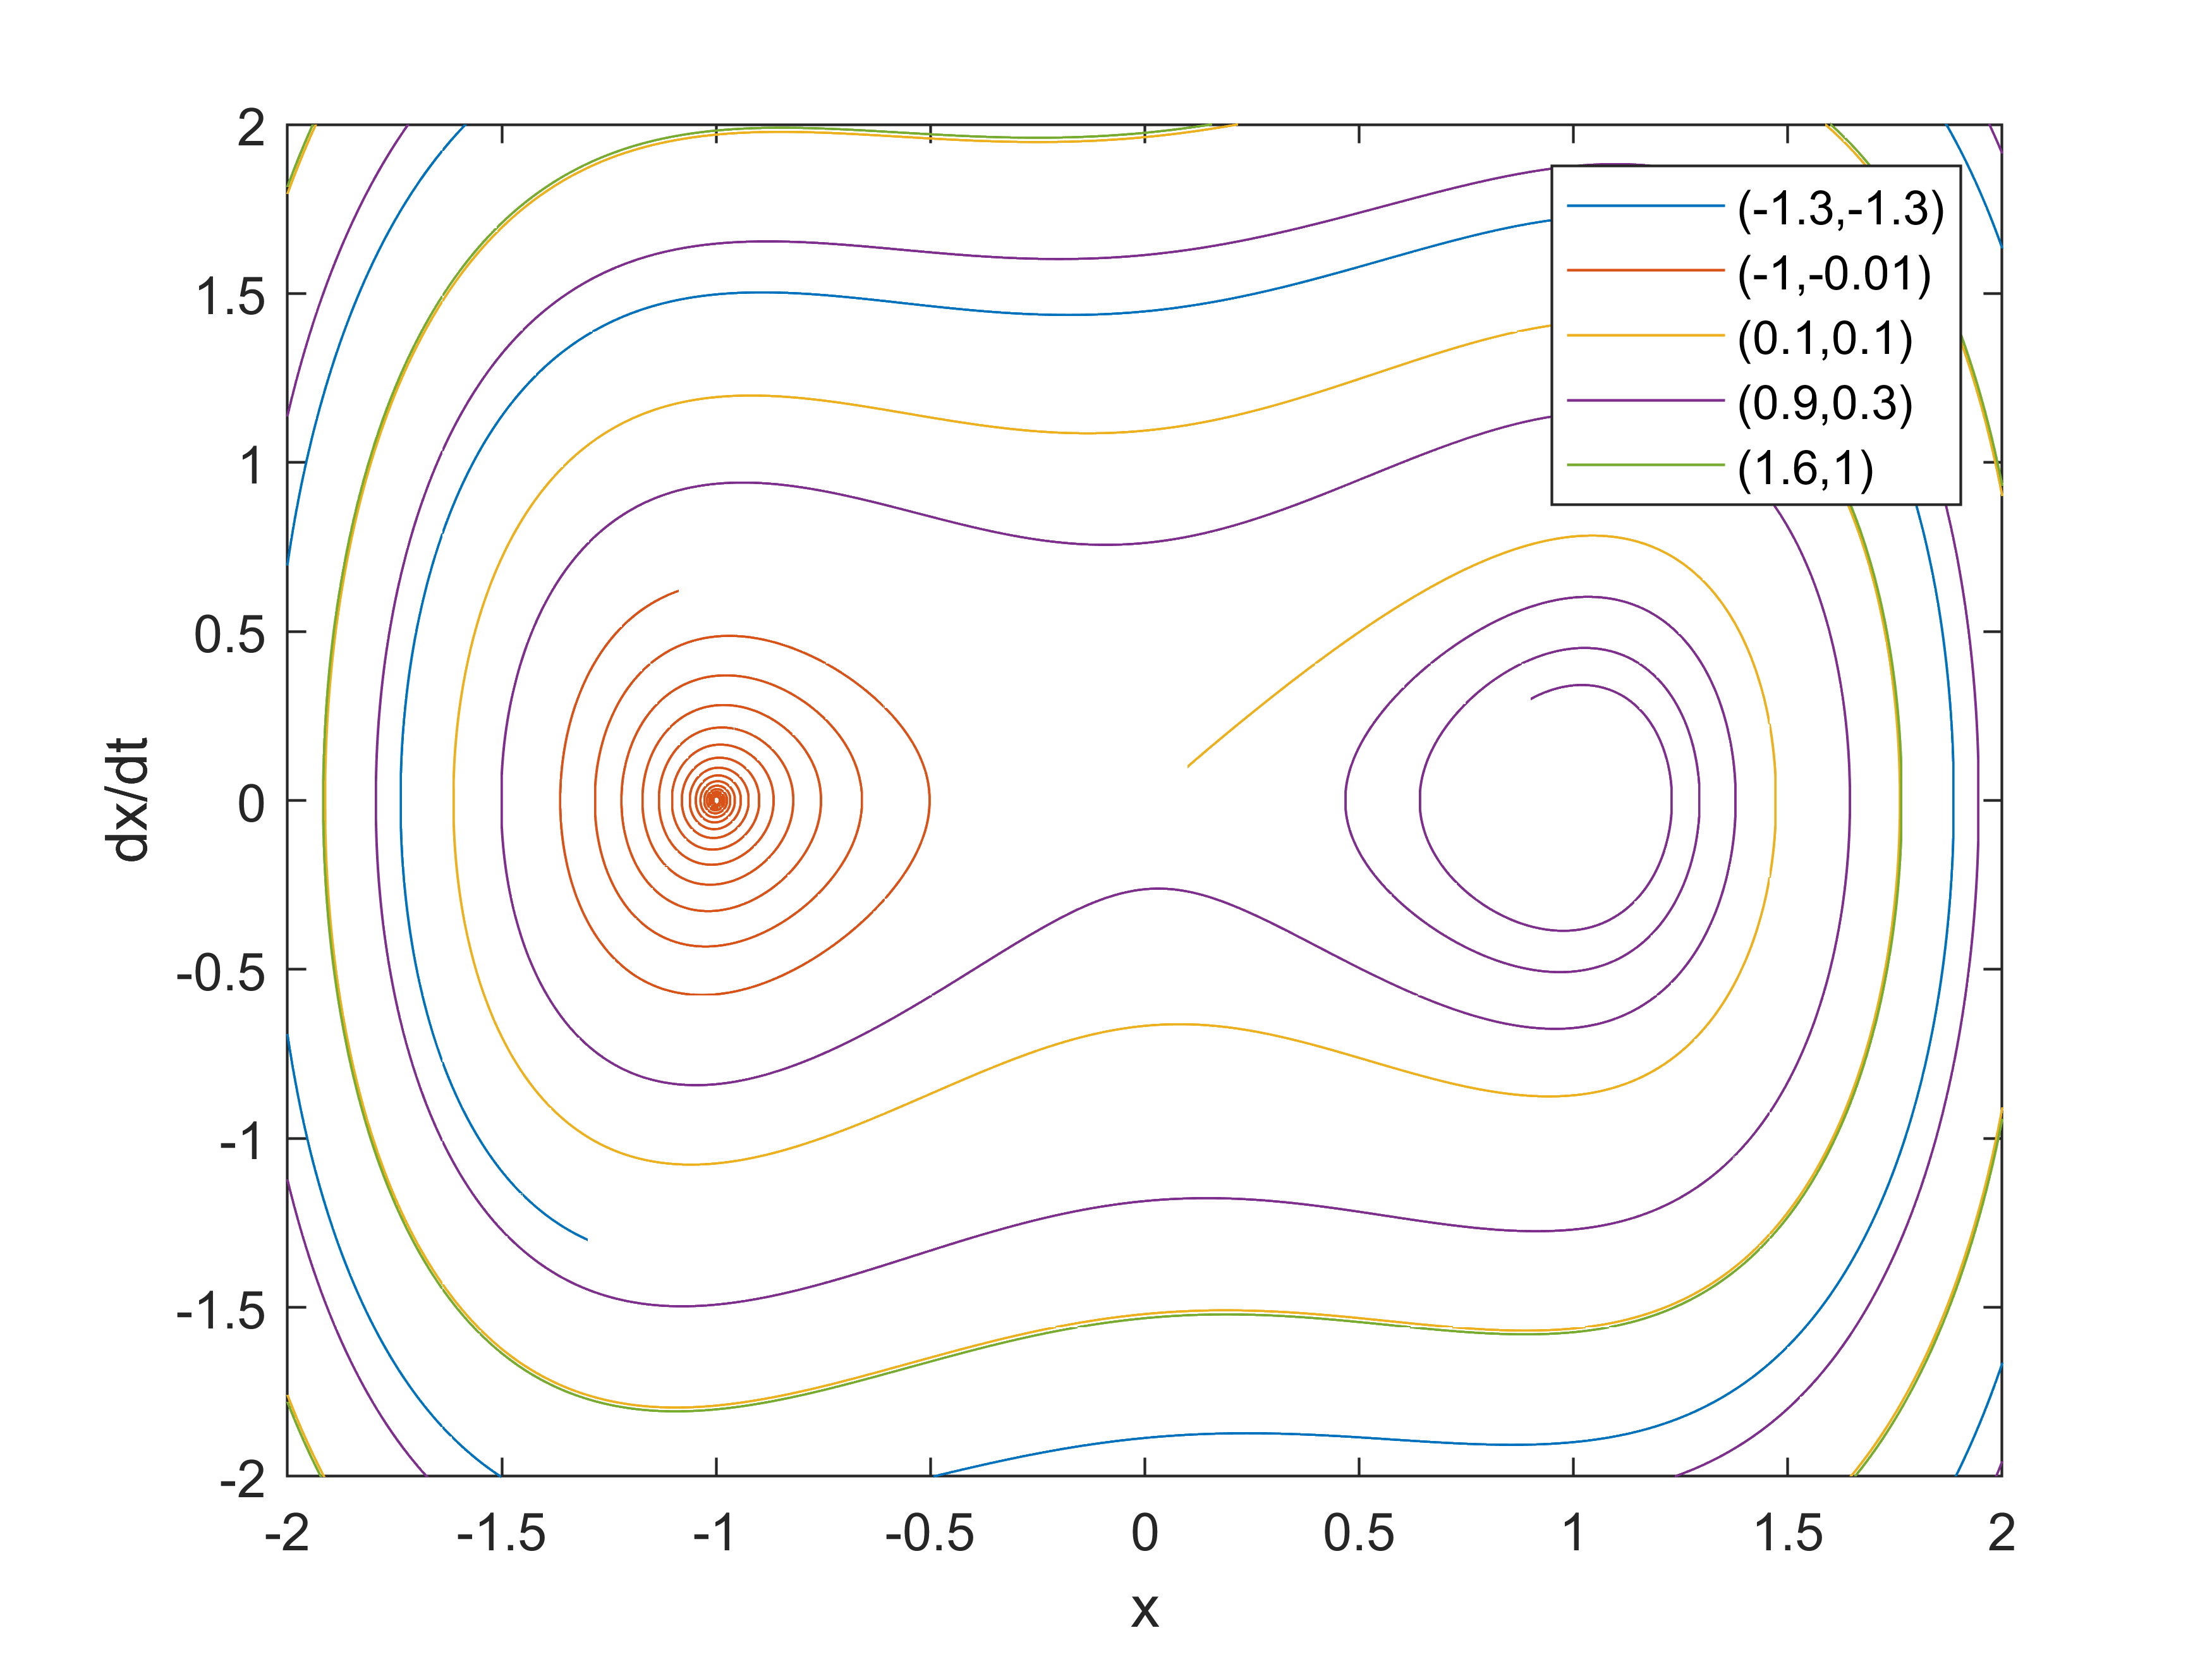
\includegraphics[width=0.5\textwidth]{Files/q1,a=-012.png}
\caption{Graph of x(t) against $\dot{x}(t)$ for $b=0, a=-0.12$}
\end{figure}
\noindent We note that as $t$ increases, the trajectories diverge from their initial conditions. This is as expected, since the fixed points at $(\pm1,0)$ are unstable foci. The trajectories follow a spiralling-out path around both both foci and the saddle point at $(0,0)$, and the radial distance to the origin increases as $t$ increases. And as $t$ increases, the value of $\frac{dx}{dt}$ changes much faster than the value of $x$, this elongates the 'oval' shaped trajectory in the $y=\frac{dx}{dt}$ direction of the graph. 

\begin{figure}[ht]
\centering
\textbf{$b=0,a=0$}\par
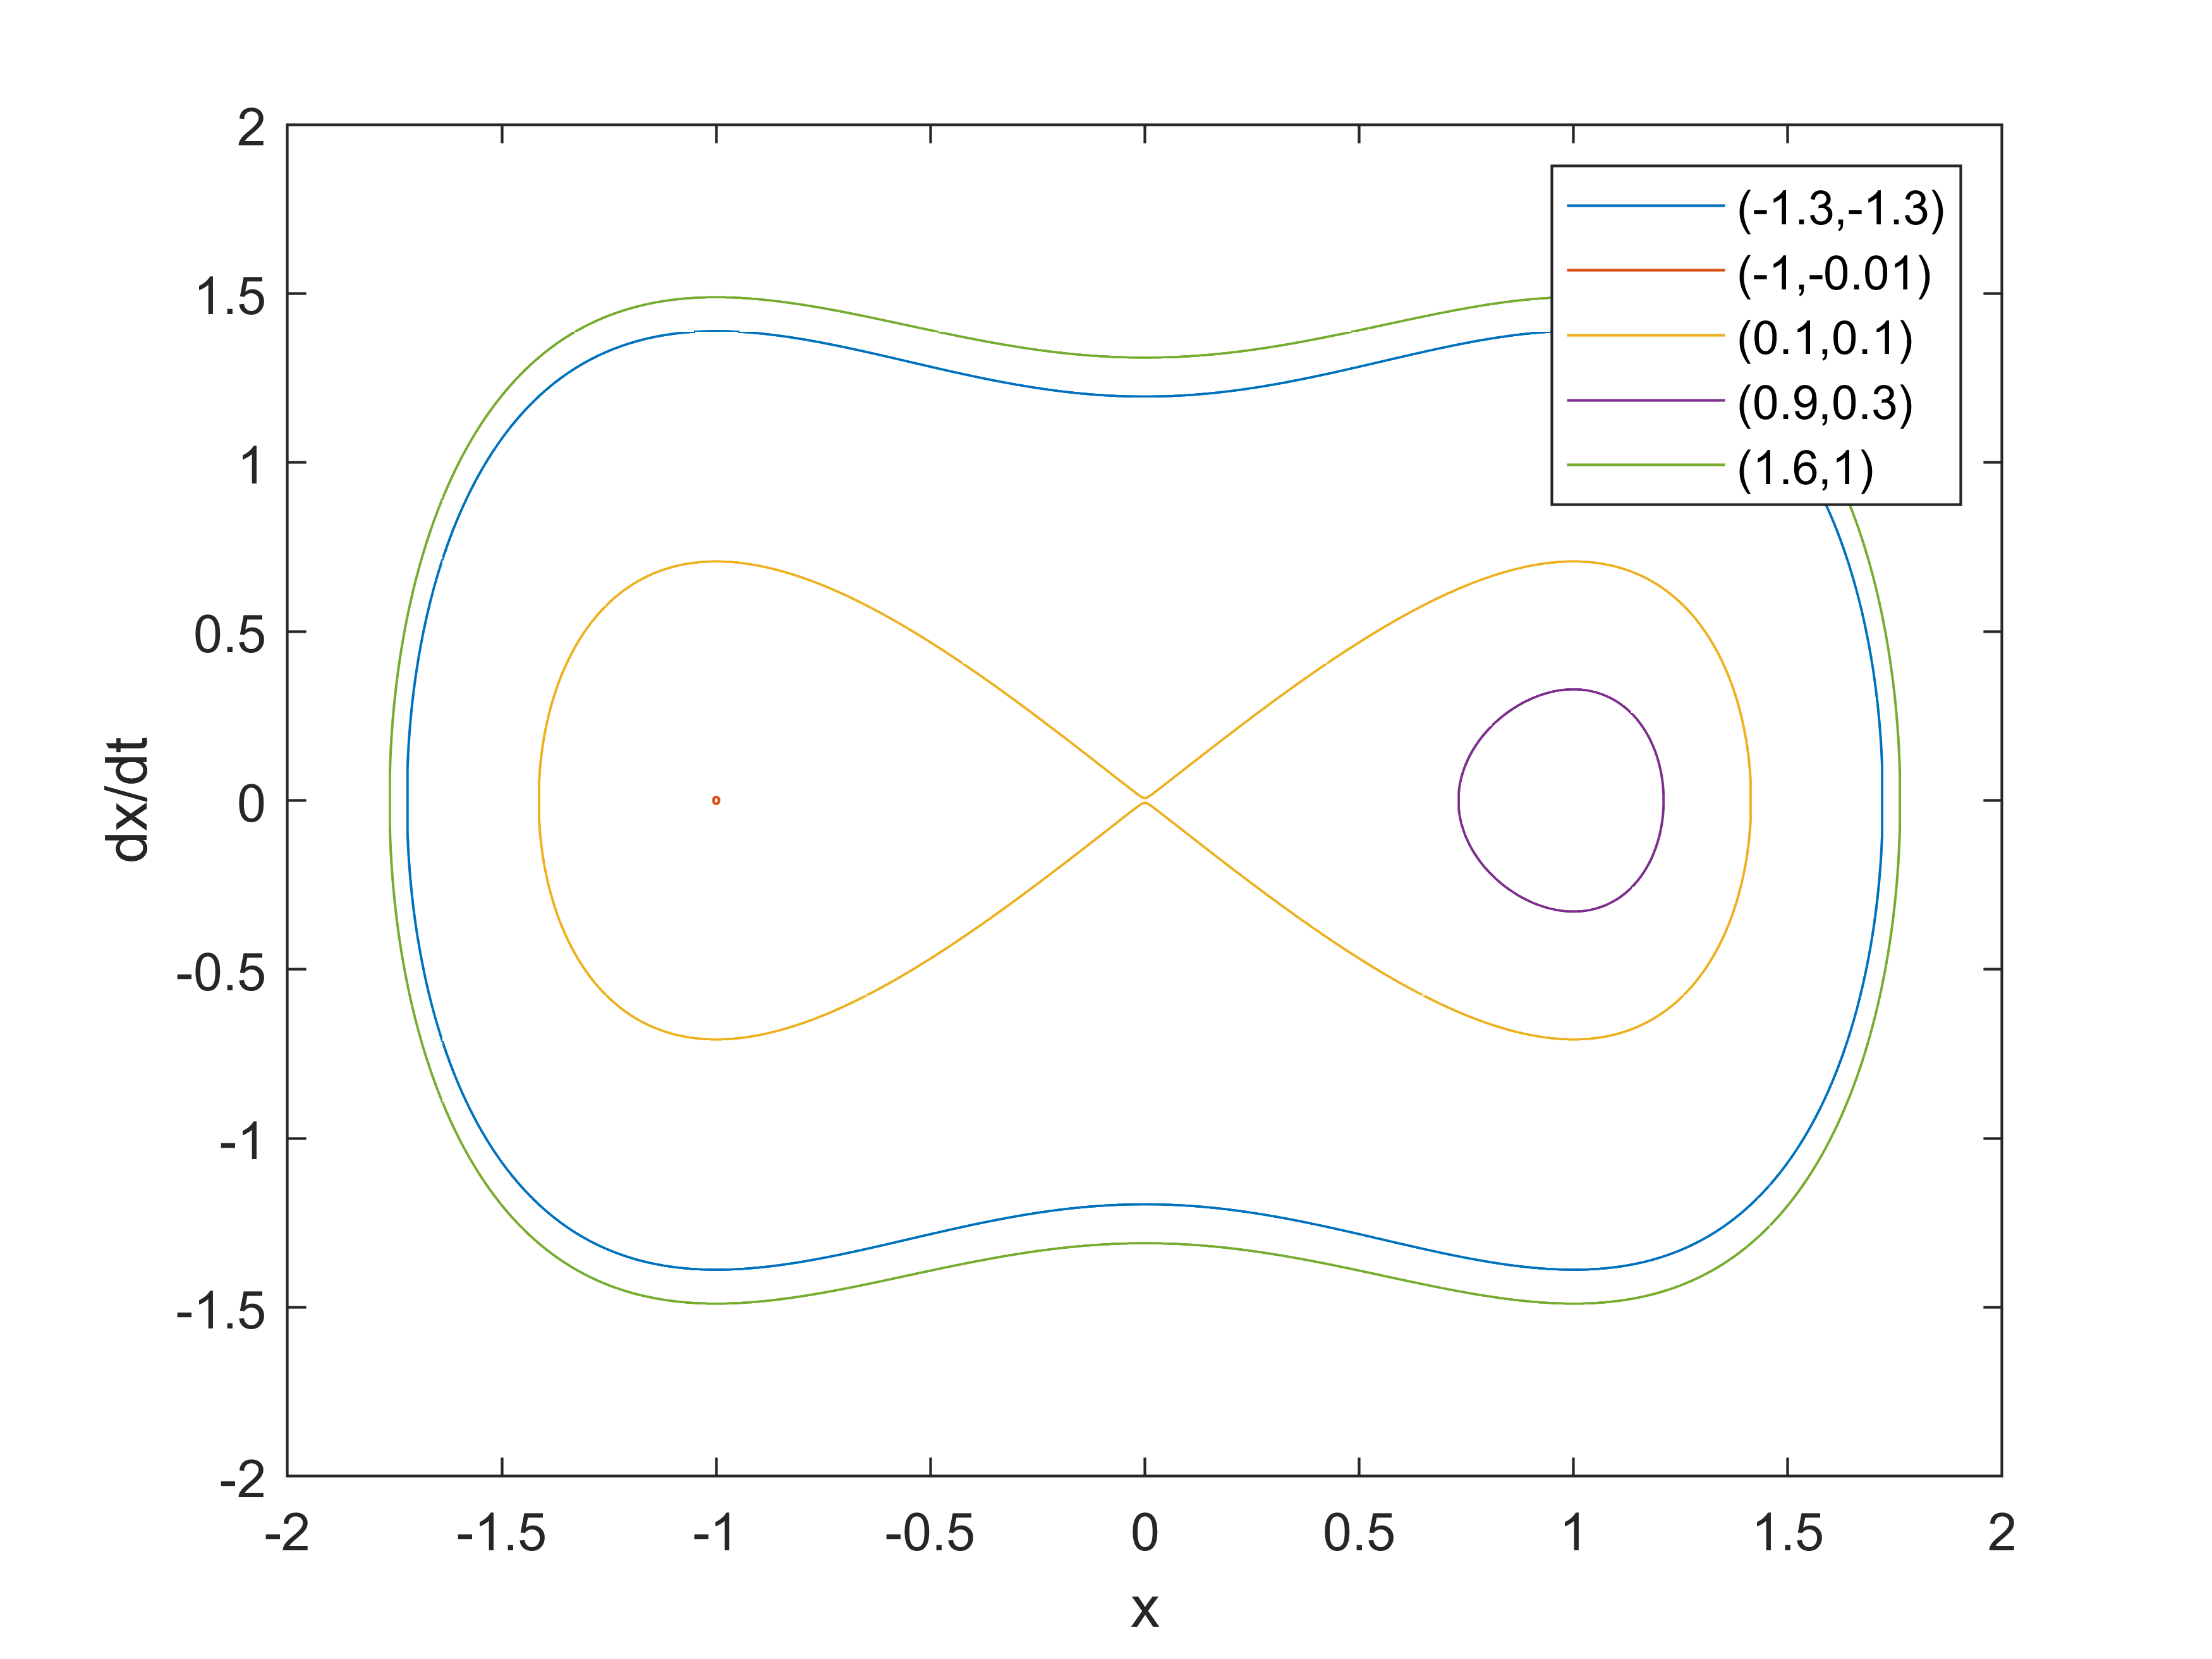
\includegraphics[width=0.5\textwidth]{Files/q1,a=0.png}
\caption{Graph of x(t) against $\dot{x}(t)$ for $b=0, a=0$}
\end{figure}
\noindent We note that the trajectories from all initial conditions are periodic orbits. This is because when $a=0$, the system we have is actually an Hamiltonian system with $H=\frac{y^2}{2}+\frac{x^4}{4}-\frac{x^2}{2}$, and all trajectories are just solutions to $H=c$ where $c$ is a constant.

\newpage
\begin{figure}[H]
\centering
\textbf{$b=0,a=0.12$}\par
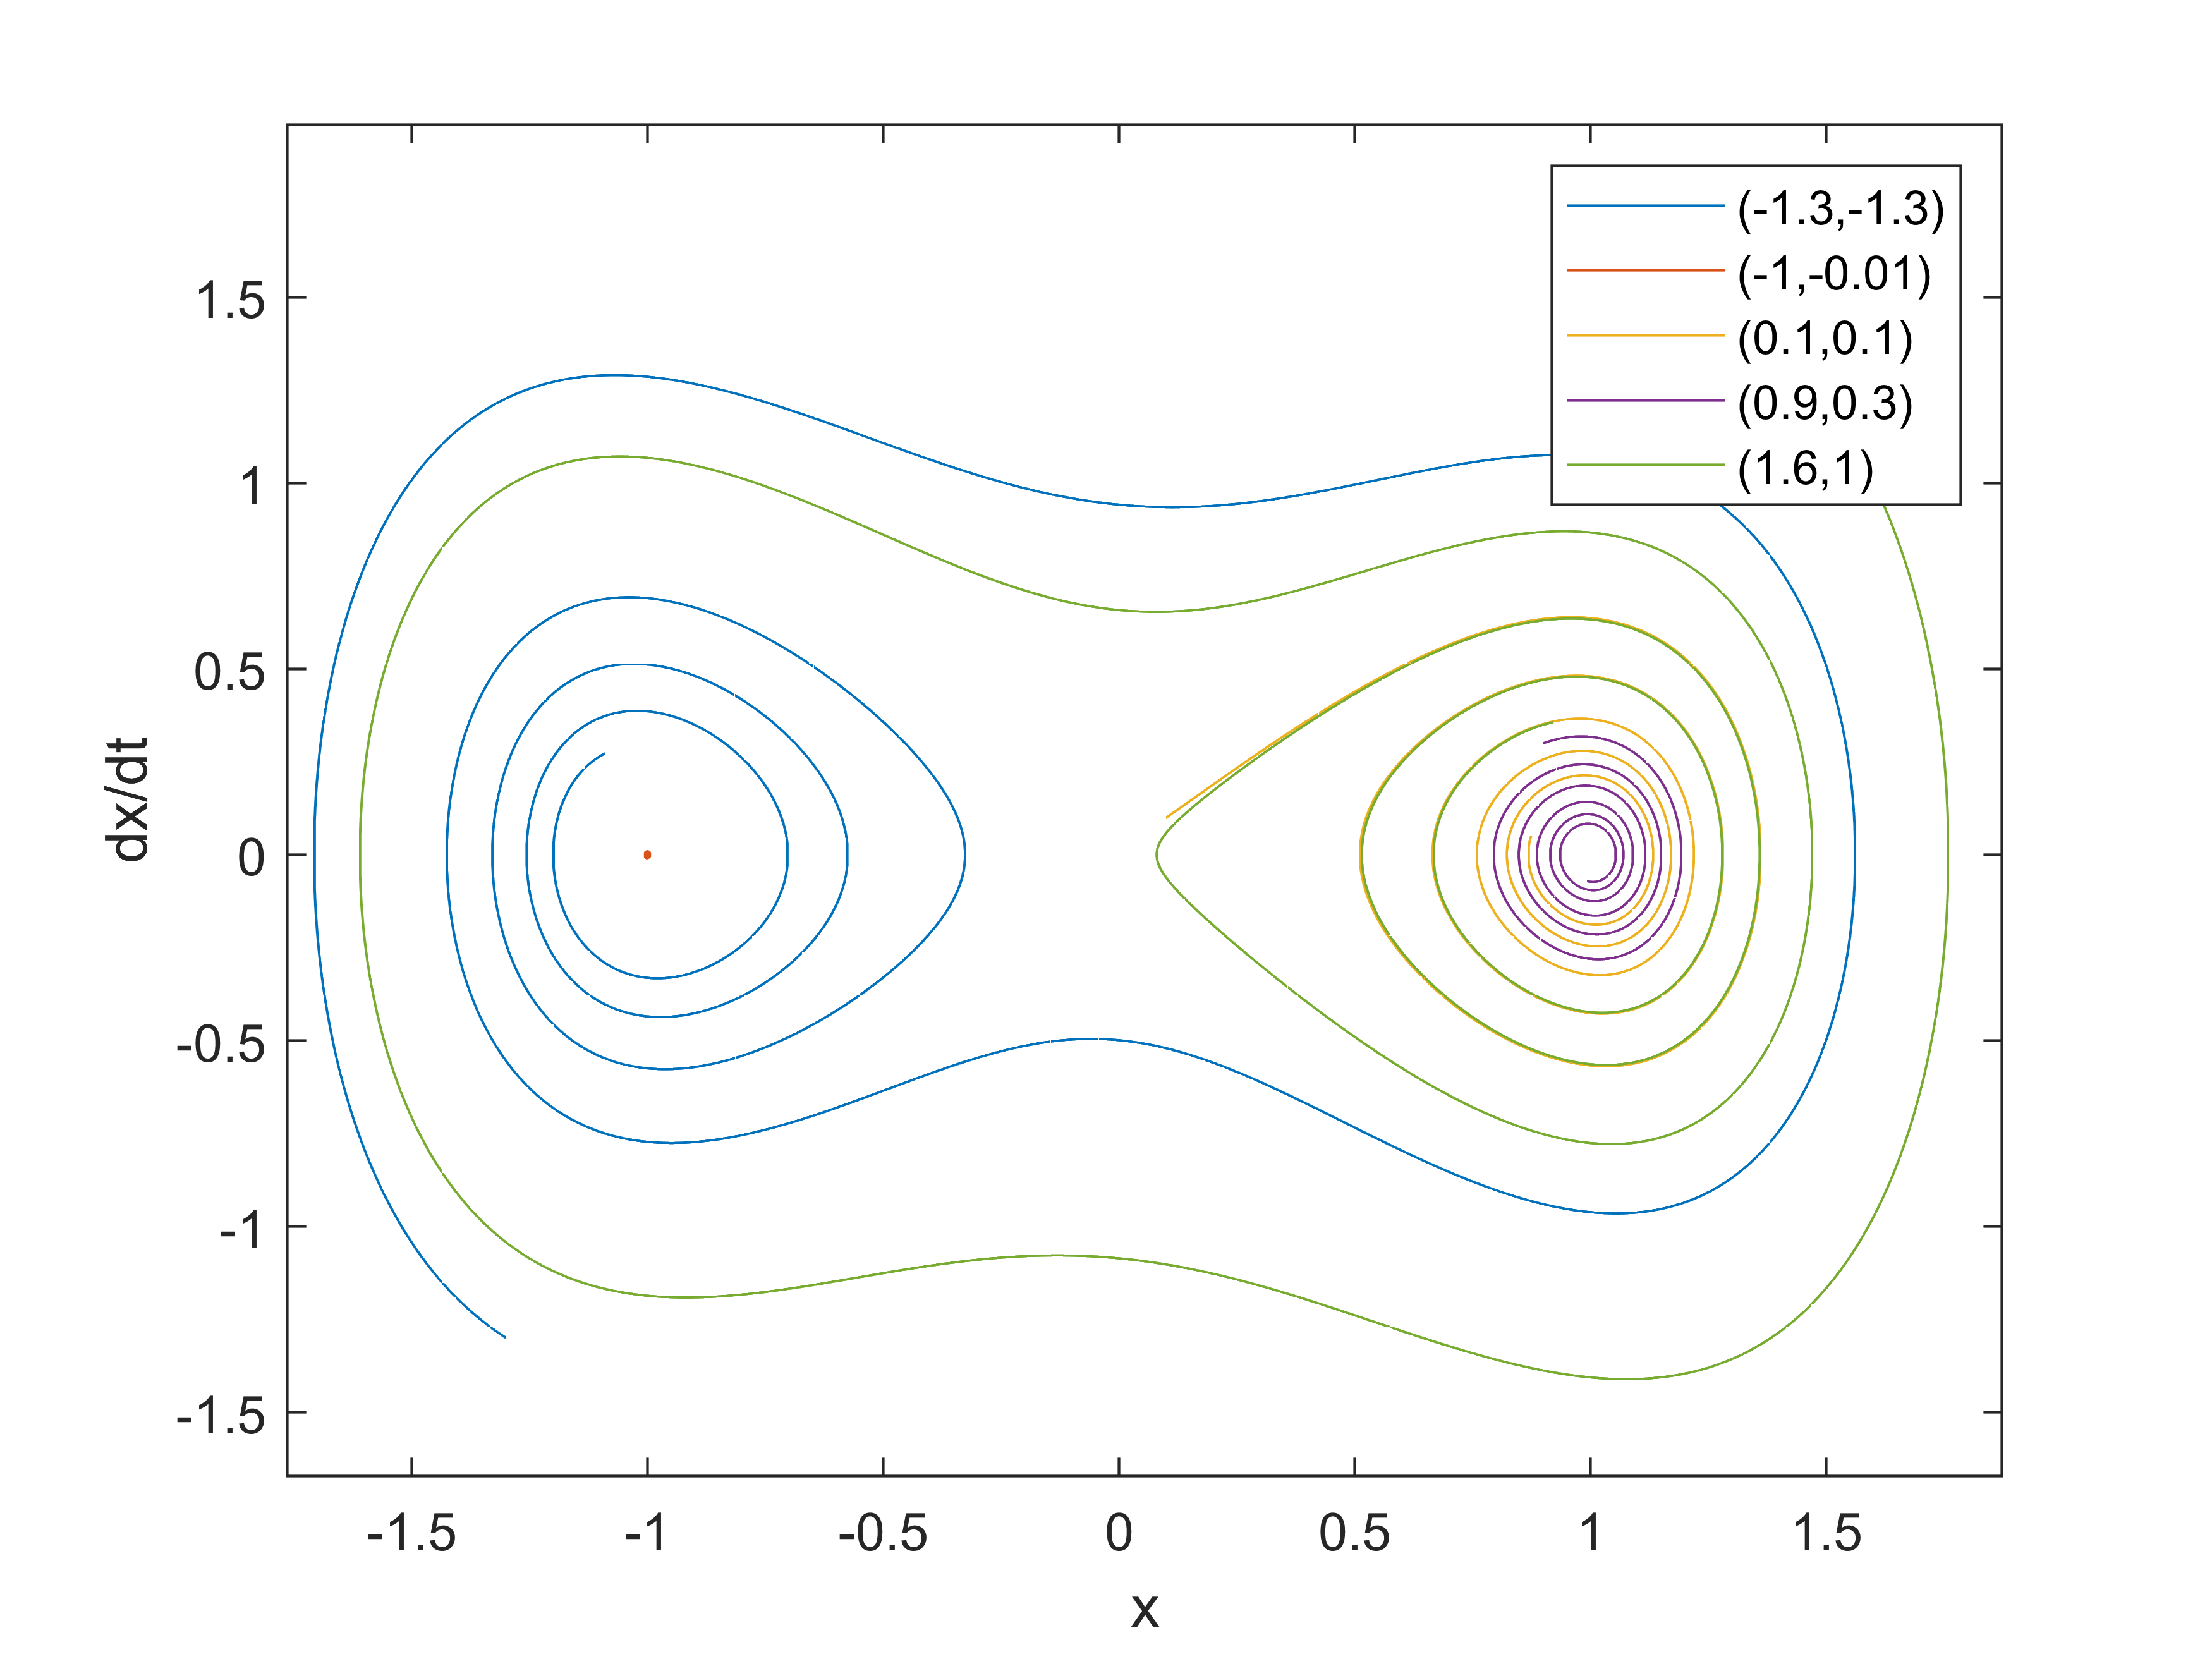
\includegraphics[width=0.5\textwidth]{Files/q1,a=012.png}
\caption{Graph of x(t) against $\dot{x}(t)$ for $b=0, a=0.12$}
\end{figure}
\noindent This is very similar to the case where $a=-0.12$, the difference is that instead of the trajectories spiralling out, they are actually spiralling in into one of the two stable foci at $(\pm1,0)$.\\\\
\noindent Note, for better clarity of the graphs, a different ending point of $t$ is chosen for different graphs, but this doesn't affect the validity of the diagrams. For $a=-0.12,0$, $t_{end}=70$; for $a=0.12$, $t_{end}=25$. This is done by changing the variable called 'endpoint' on line 7 of the program.\\ 

\subsection*{Question 3}
We make slight changes to the program used in question 1 for this question, for simplicity of testing, it's written to a separate file and can be found in the programs section under the title \emph{'ii) q3.m'}.\\
The initial conditions chosen are $(x(0),\dot{x}(0))=(-1.5,2)$ and $(0.01,0.01)$ and their trajectories are plotted in blue and red respectively. We can see that the blue trajectory tends towards a periodic orbit whereas the red trajectory looks like a "strange attractor" as it never appear to settle down to any simple closed loop.
\begin{figure}[ht]
\centering
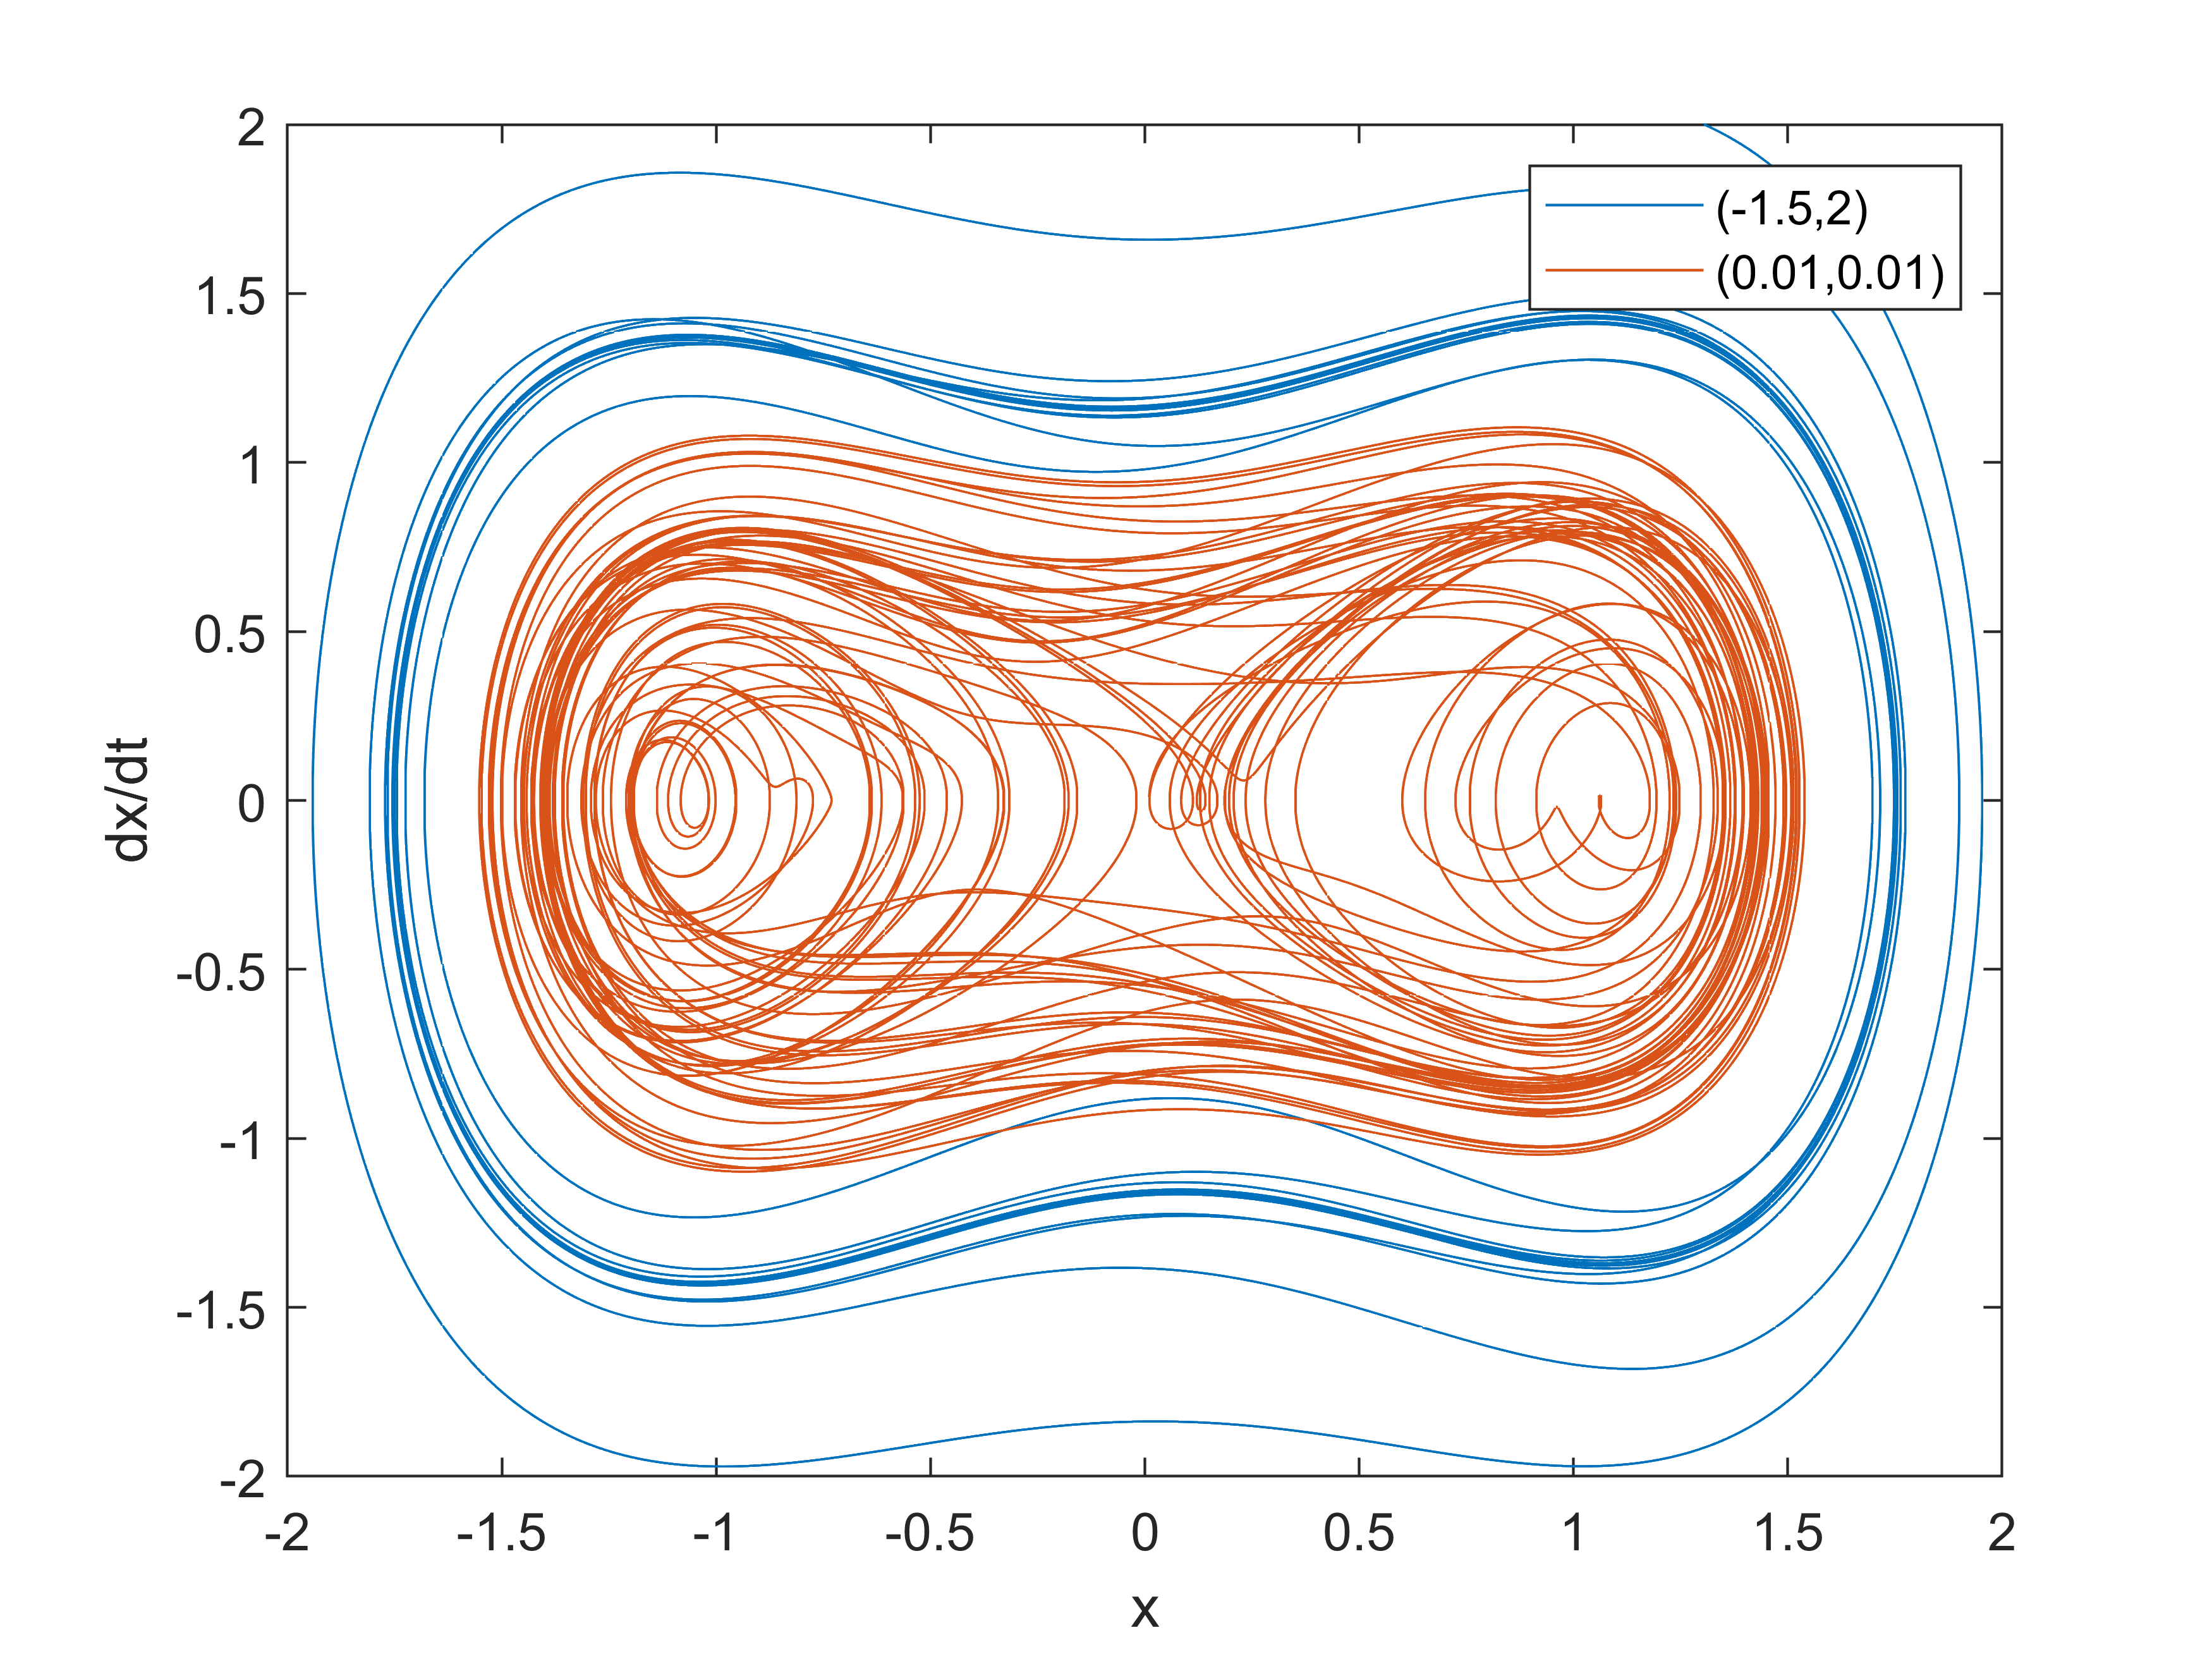
\includegraphics[width=0.5\textwidth]{Files/q3.png}
\caption{Graph of x(t) against $\dot{x}(t)$ for $b=0.3, a=0.15$}
\end{figure}

\newpage
\subsection*{Question 4}
The program used to plot the graph below can be found in the programs section under the title \emph{'iii) q4.m'}.
\begin{figure}[ht]
\centering
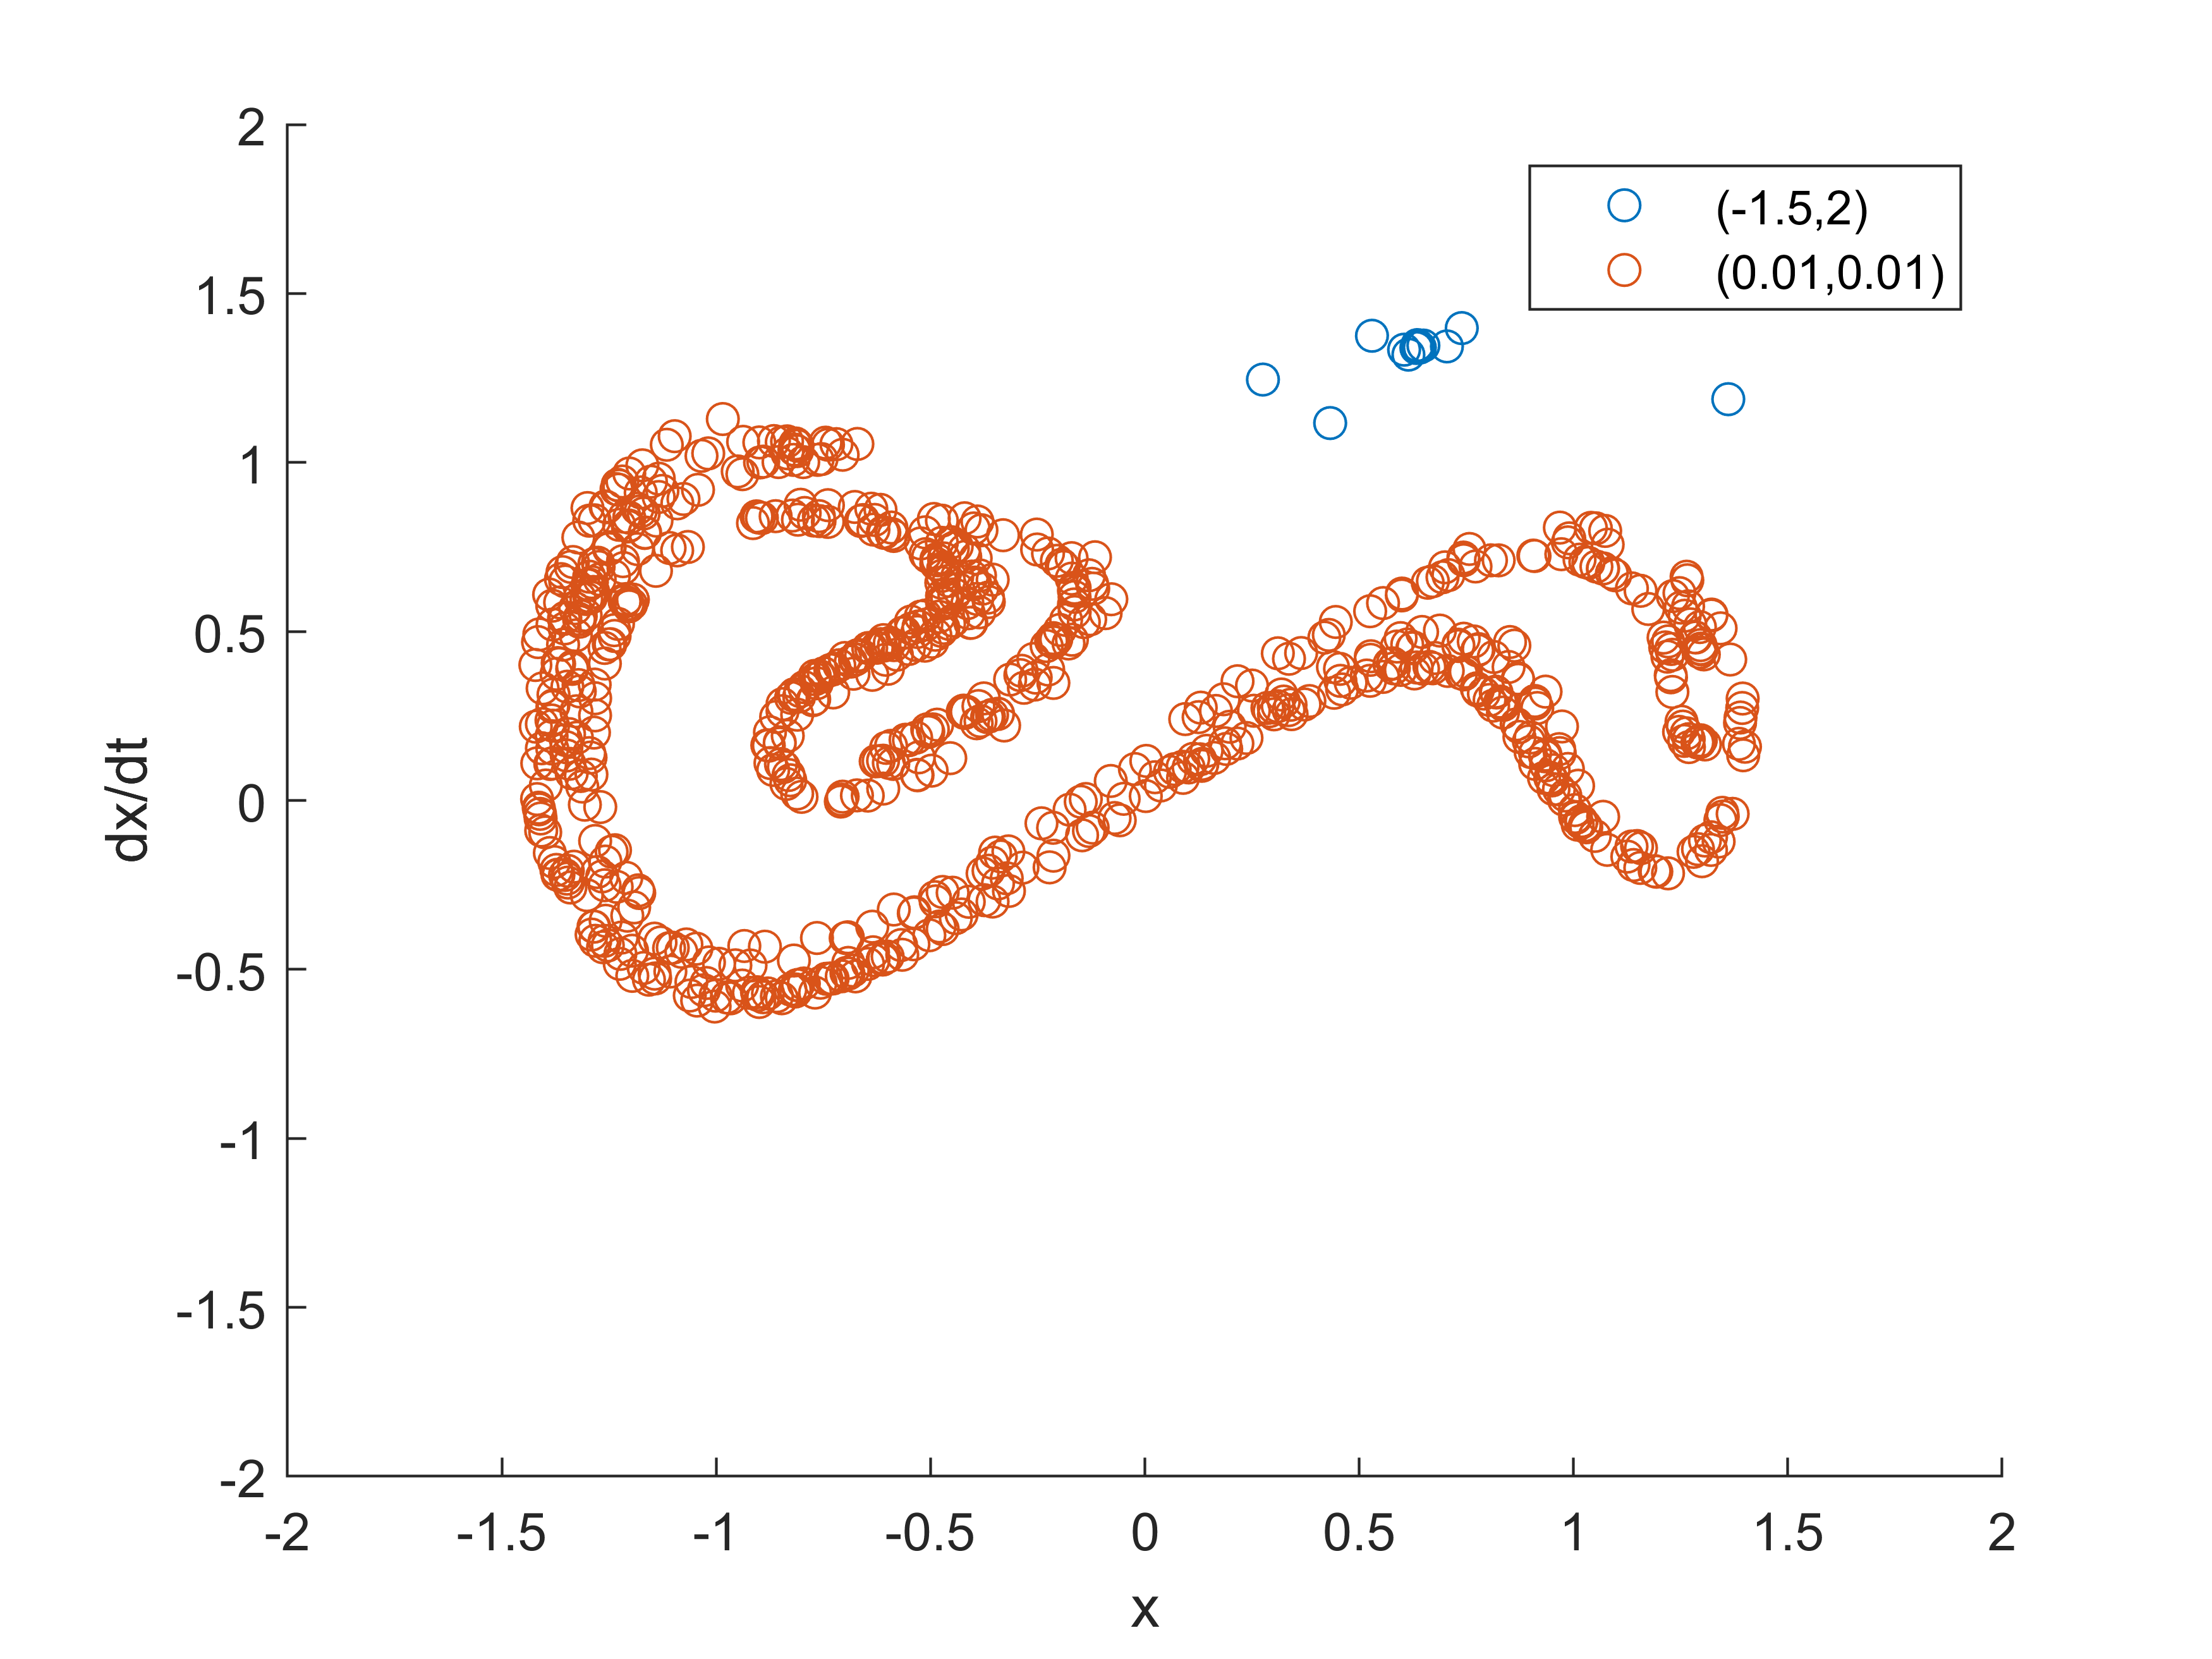
\includegraphics[width=0.45\textwidth]{Files/q4.png}
\caption{Graph of x(t) against $\dot{x}(t)$ for $b=0.3, a=0.15$ at $t=2k\pi$}
\end{figure}\\
We note when plotting only points at $t=2k\pi$, we can still see part of the orbit of the strange attractor (red), but only some points of the periodic orbit (blue) concentrated around $(0.6,1.3)$.\\
The reason why the blue points seem to concentrate at one place is because the solutions tends to a periodic orbit, and the periodic orbit has period $2\pi$, as the equation has a periodic forcing term $b\cos t$ which has period $2\pi$. Therefore, once $k$ is large enough, $\phi_{2k\pi}(x,\frac{dx}{dt})\approx\phi_{2(k+1)\pi}(x,\frac{dx}{dt})$.\\
We are still able to see parts of the trajectory of the strange attractor because it's non-periodic and hence $t=2k\pi$ would lead to all different points.\\
And therefore, to identify the periodic orbit, it's better to plot out the whole trajectory, however, if we wish to see which points each $t$ value corresponds to on the periodic orbit, it could be better to plot by points.\\
Therefore, to identify the coordinate/shape of the periodic orbit, it's better to plot out the whole trajectory, however, if we wish to see which points each $t$ value corresponds to on the periodic orbit or if a periodic orbit exists, it could be better to plot by points.

\subsection*{Question 5}
In this question, we first plot a bifurcation diagram.
\begin{figure}[H]
\centering
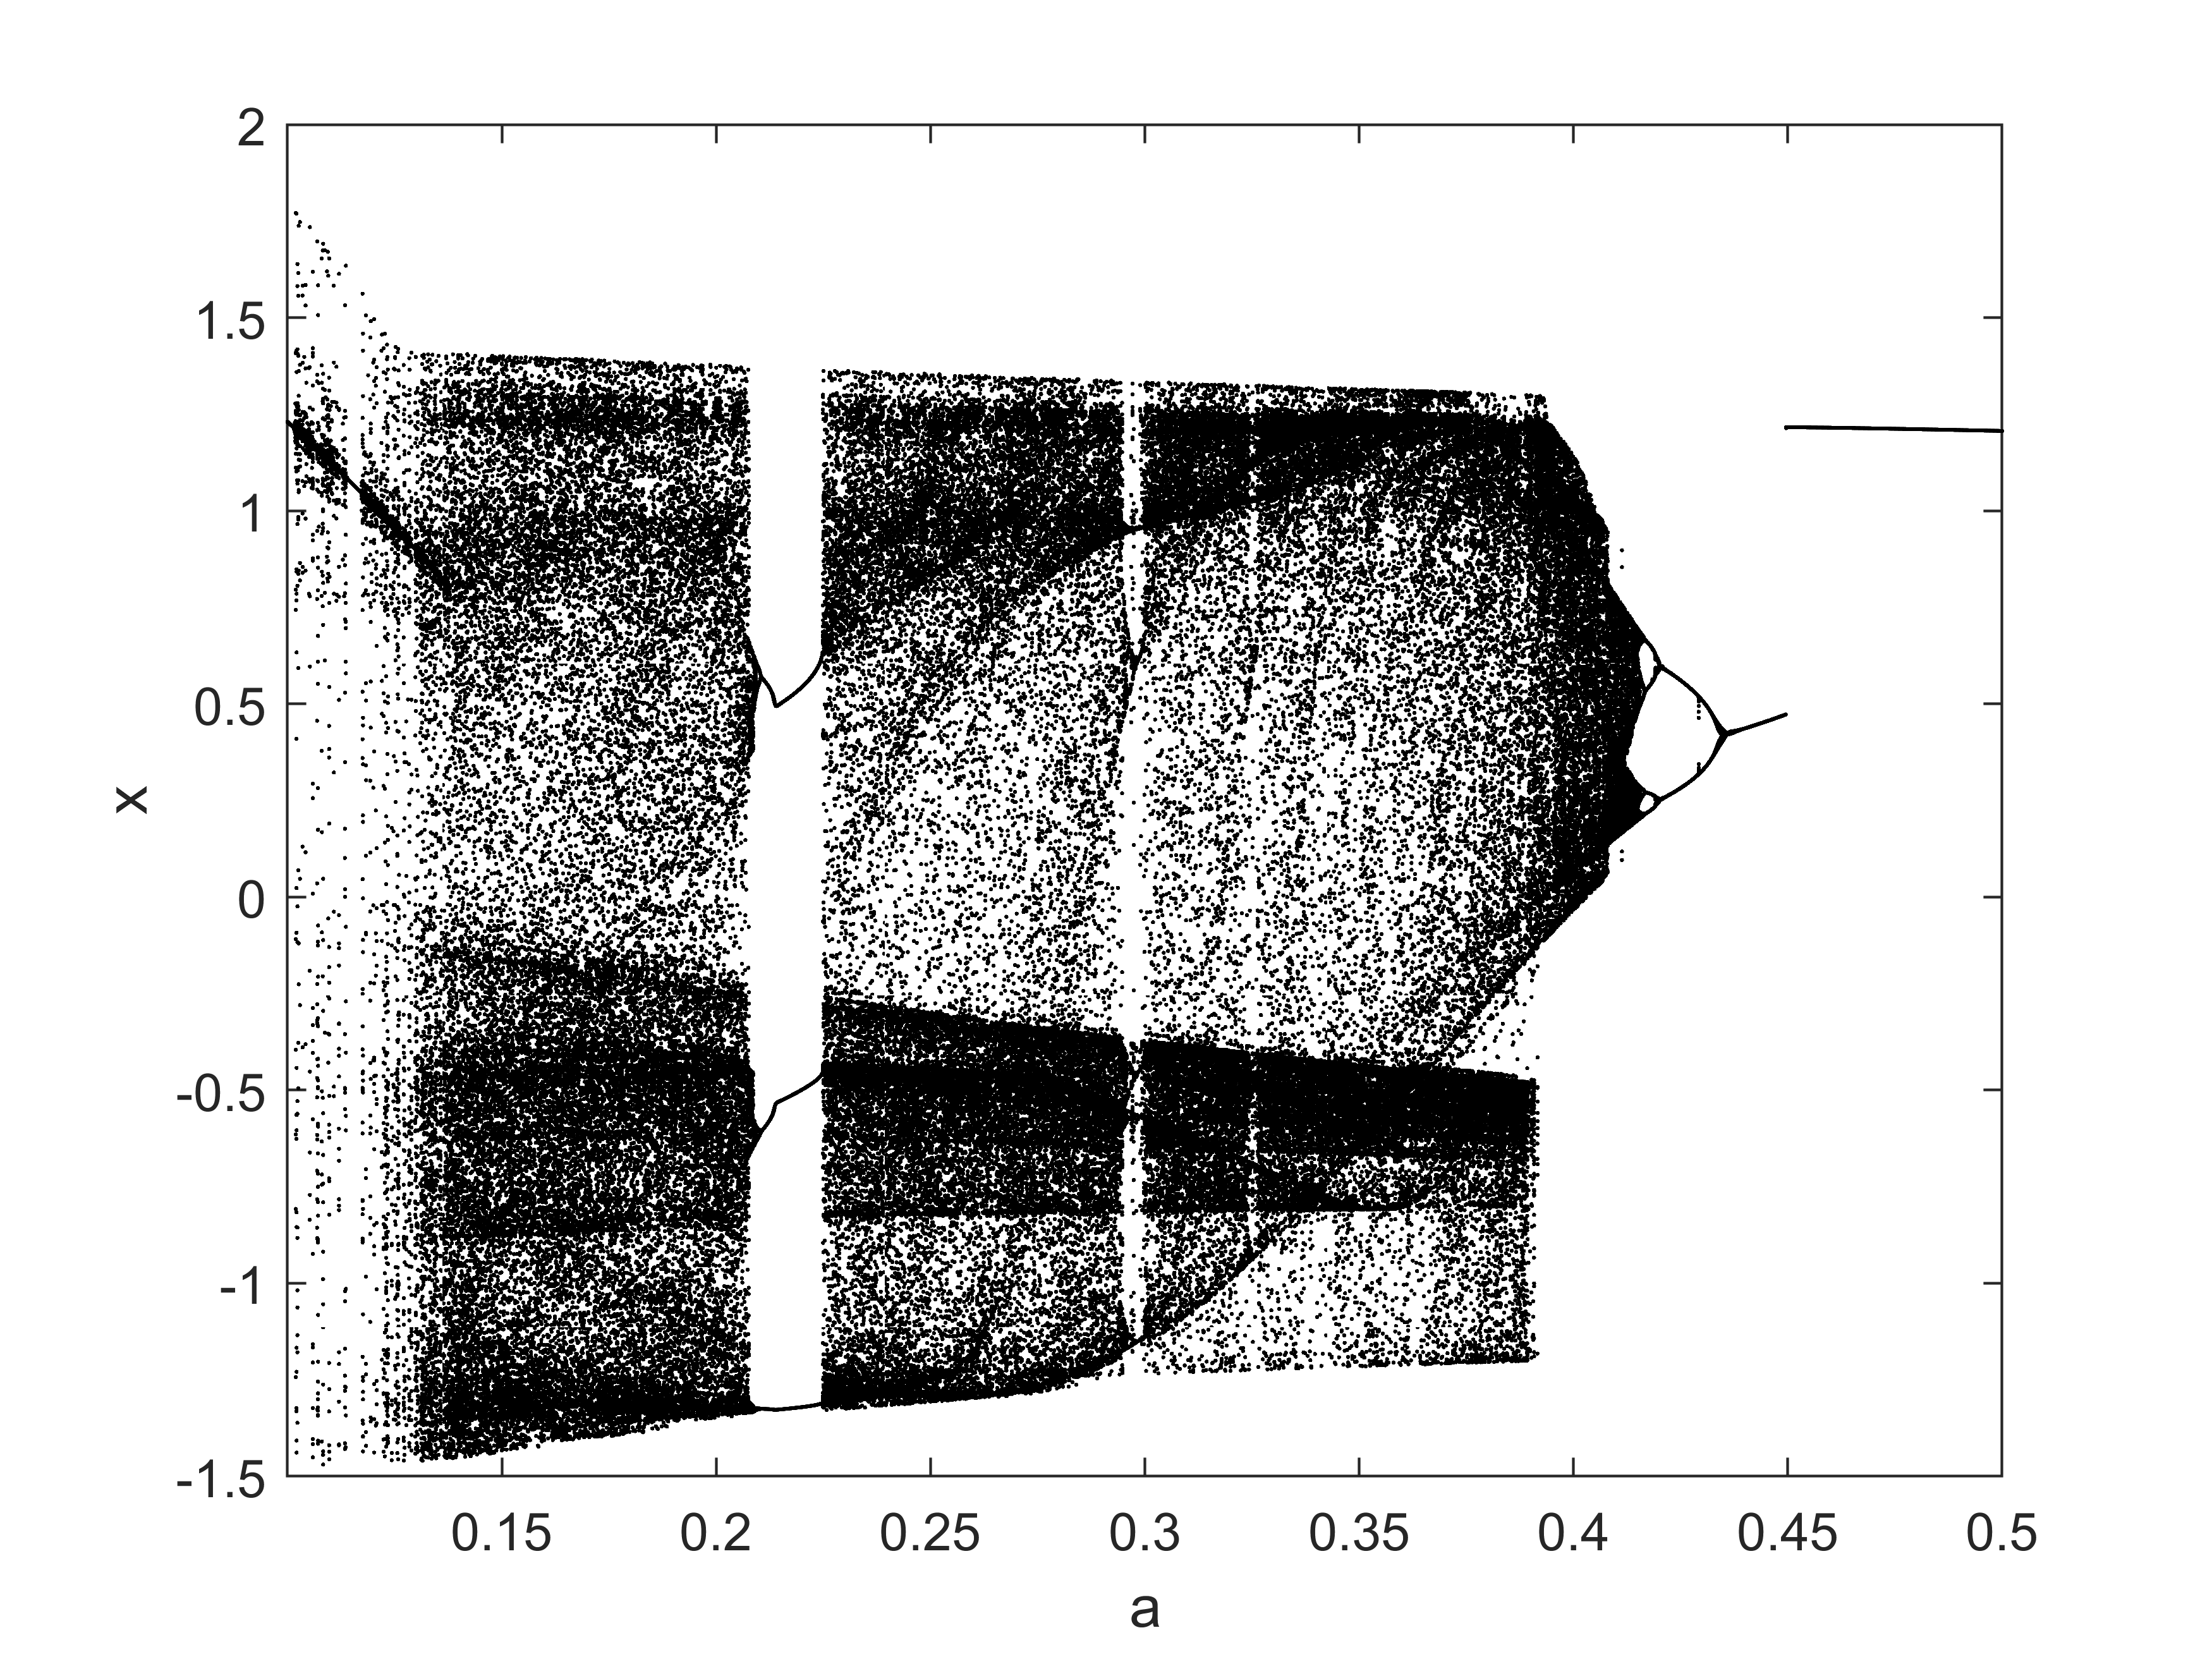
\includegraphics[width=0.55\textwidth]{Files/q5.png}
\caption{Bifurcation diagram of $x$ against $a\in(0.1,0.5)$}
\end{figure}
\noindent To do this, we use the program \emph{'iv) q5\textunderscore bifurcation.m'}. We first fix some initial conditions. In this graph, it's $(x,y)=(0.1,0.1)$. We then numerically integrate the equations to $t=500$ with $h=0.0001$. We then plot the last 'nplot' ($50$ in this case) points of $x(t)$ at $t=2n\pi$. We repeat this process from $a=0.1$ to $a=0.5$, each time we increment $a$ by $0.0001$. Note, because we chose 'nplot' to be $50$, some of the trajectories might not have fully converged to the periodic orbit yet, which causes some blurring around bifurcation points.\\
We can see on the graph that we have a periodic orbit with period $2\pi$ at $a=0.44$. This orbit that experiences a period doubling bifurcation around $a=0.4357$, and at $a=0.423$, it has period $4\pi$. Another period doubling bifurcation occurs around $a=0.4205$, and the orbit now has period $8\pi$, e.g. at $a=0.4178$.\\
The period continues to double as value of $a$ decreases. The system becomes increasingly chaotic. And at values like $a=0.23$, the system is very chaotic. However, at around $a=0.225$, the system suddenly returns to having a periodic orbit with period $6\pi$.\\
Hence, we will plot the graph of $x(t)$ against $y(t)$ at $a=(0.44,0.423,0.4178,0.23,0.22)$.\\
We now use \textit{'v) q5\textunderscore graph.m'} to plot these graphs. This program plots both the trajectory and the points at $t=2n\pi$.\\
\begin{figure}[H]
    \begin{minipage}[b]{0.5\linewidth}
            \centering
            \textbf{a=0.44}\par
            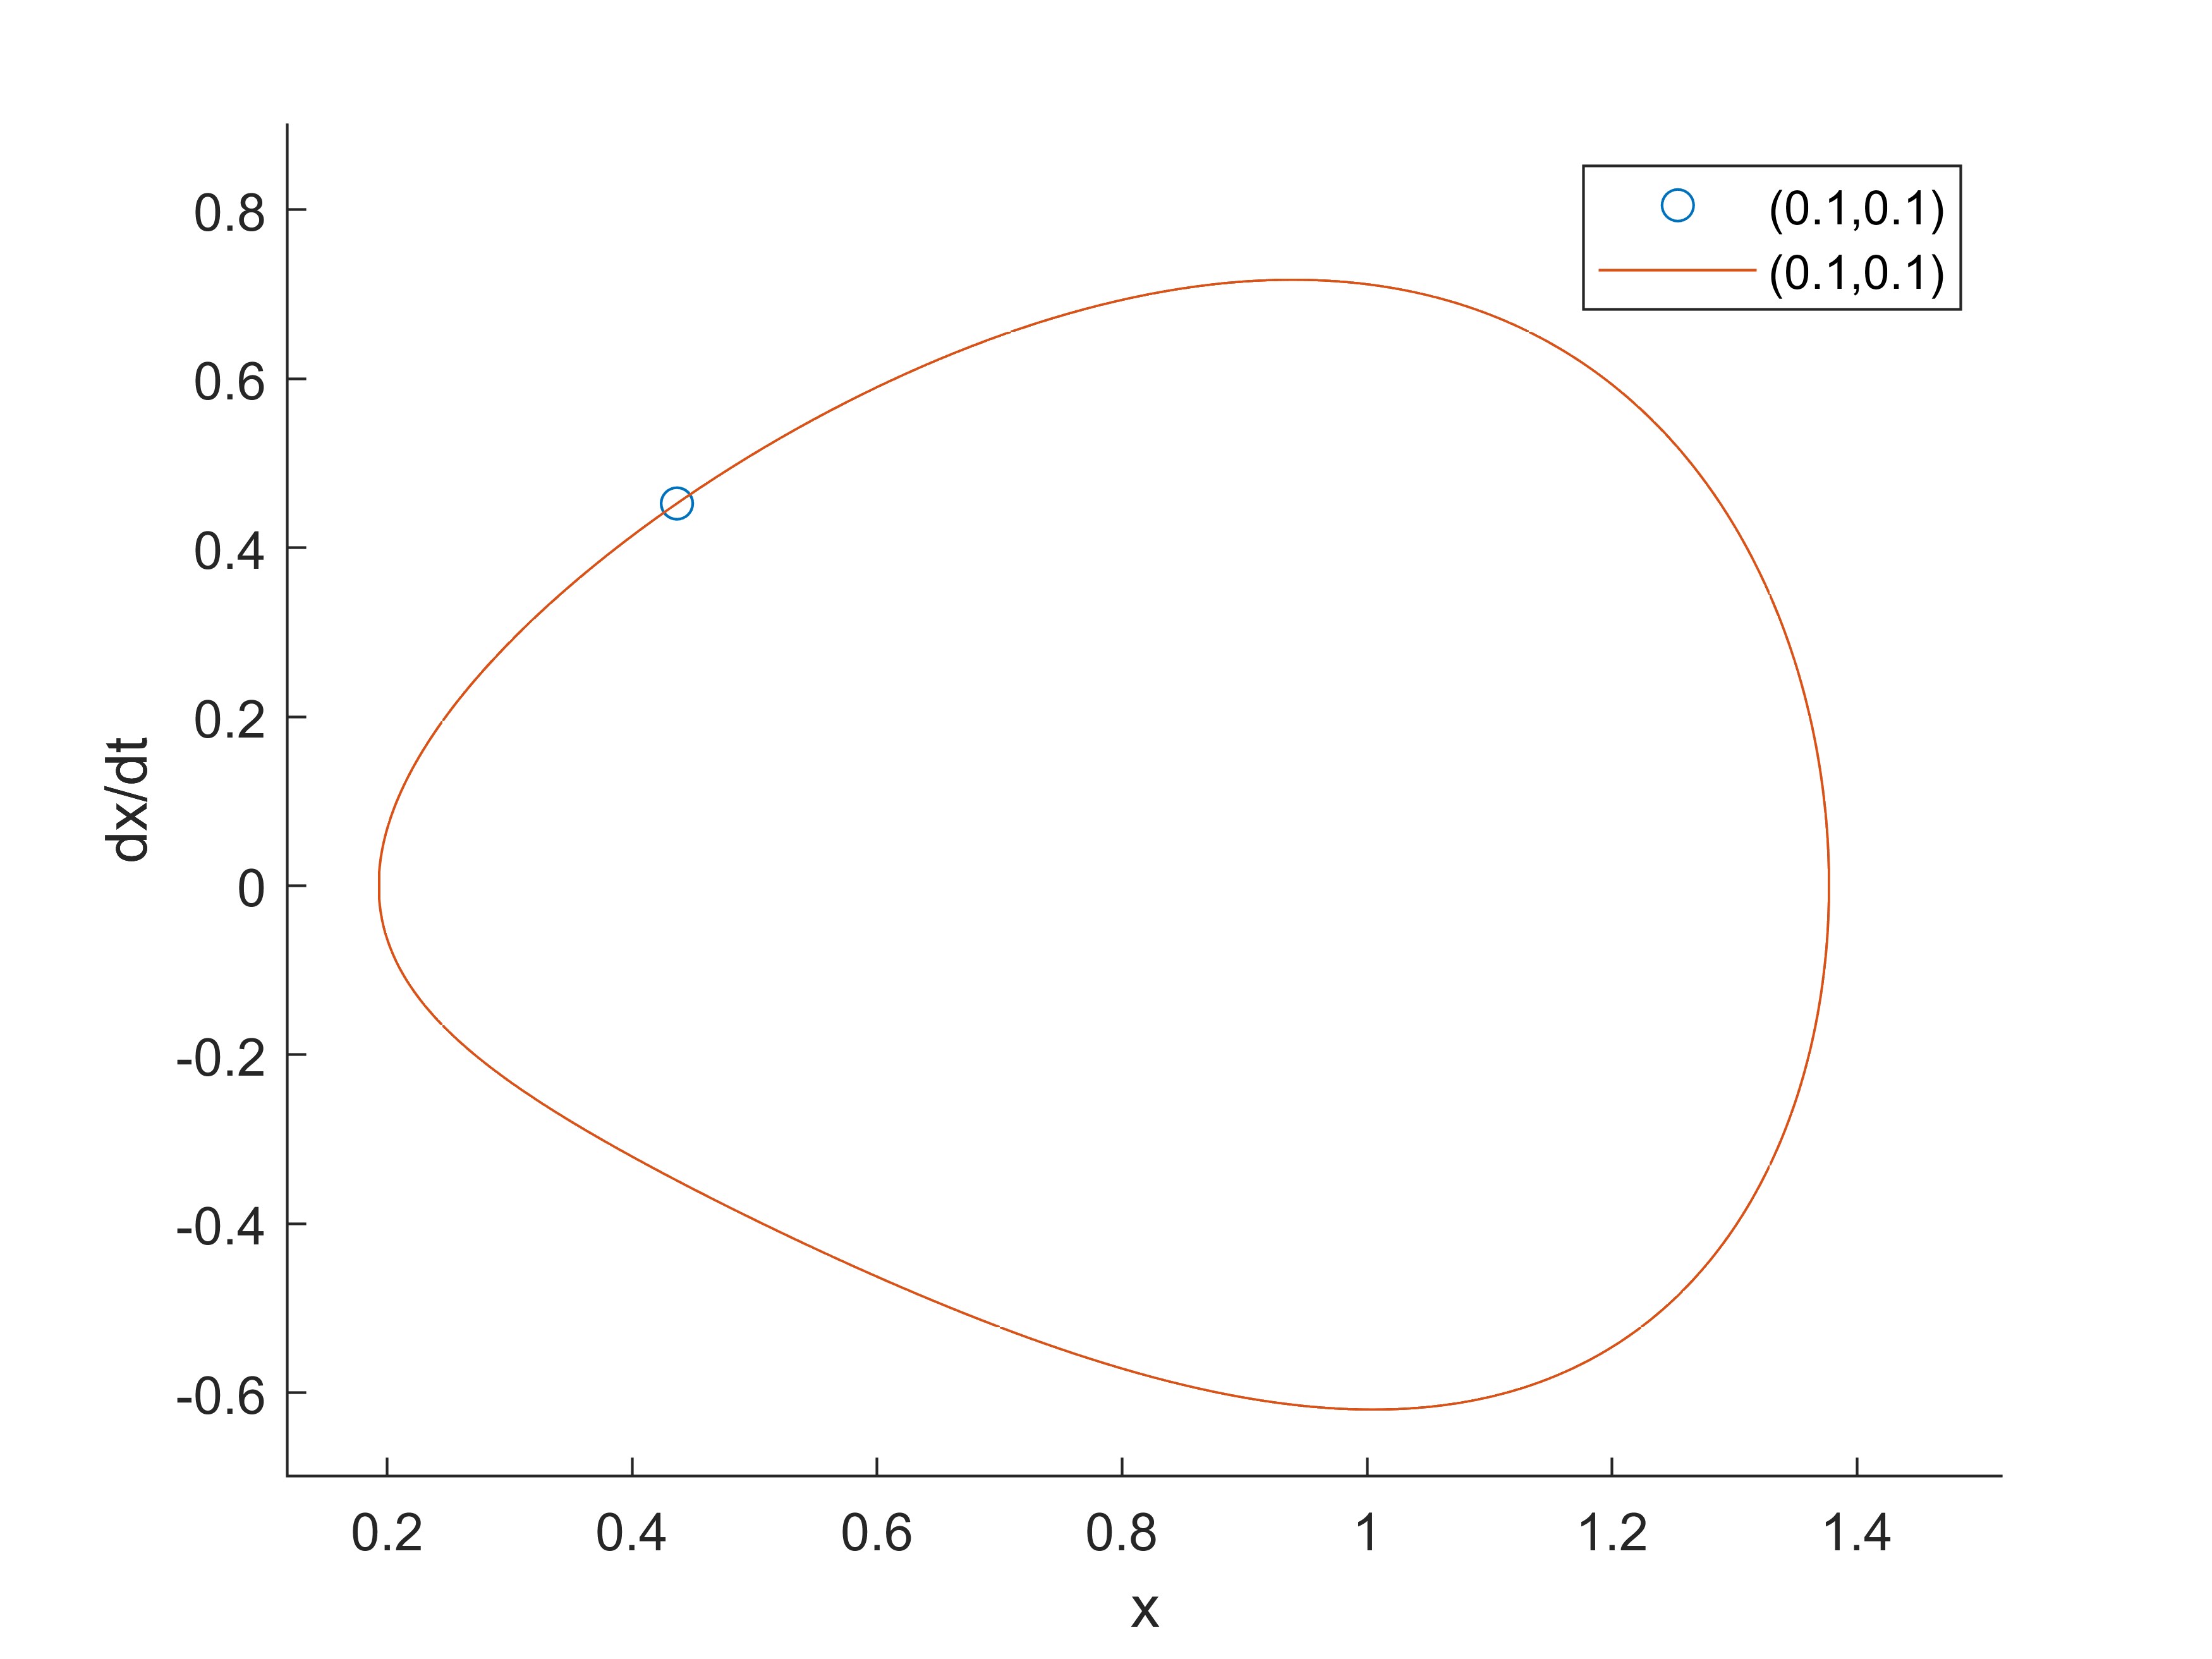
\includegraphics[width=\textwidth]{Files/q5,a=0.44.png}
            \caption{Graph of periodic orbits on x(t) against $\dot{x}(t)$ for $a=0.44$}
        \end{minipage}
        \hfill
        \begin{minipage}[b]{0.5\linewidth}
            \centering
            \textbf{a=0.423}\par
            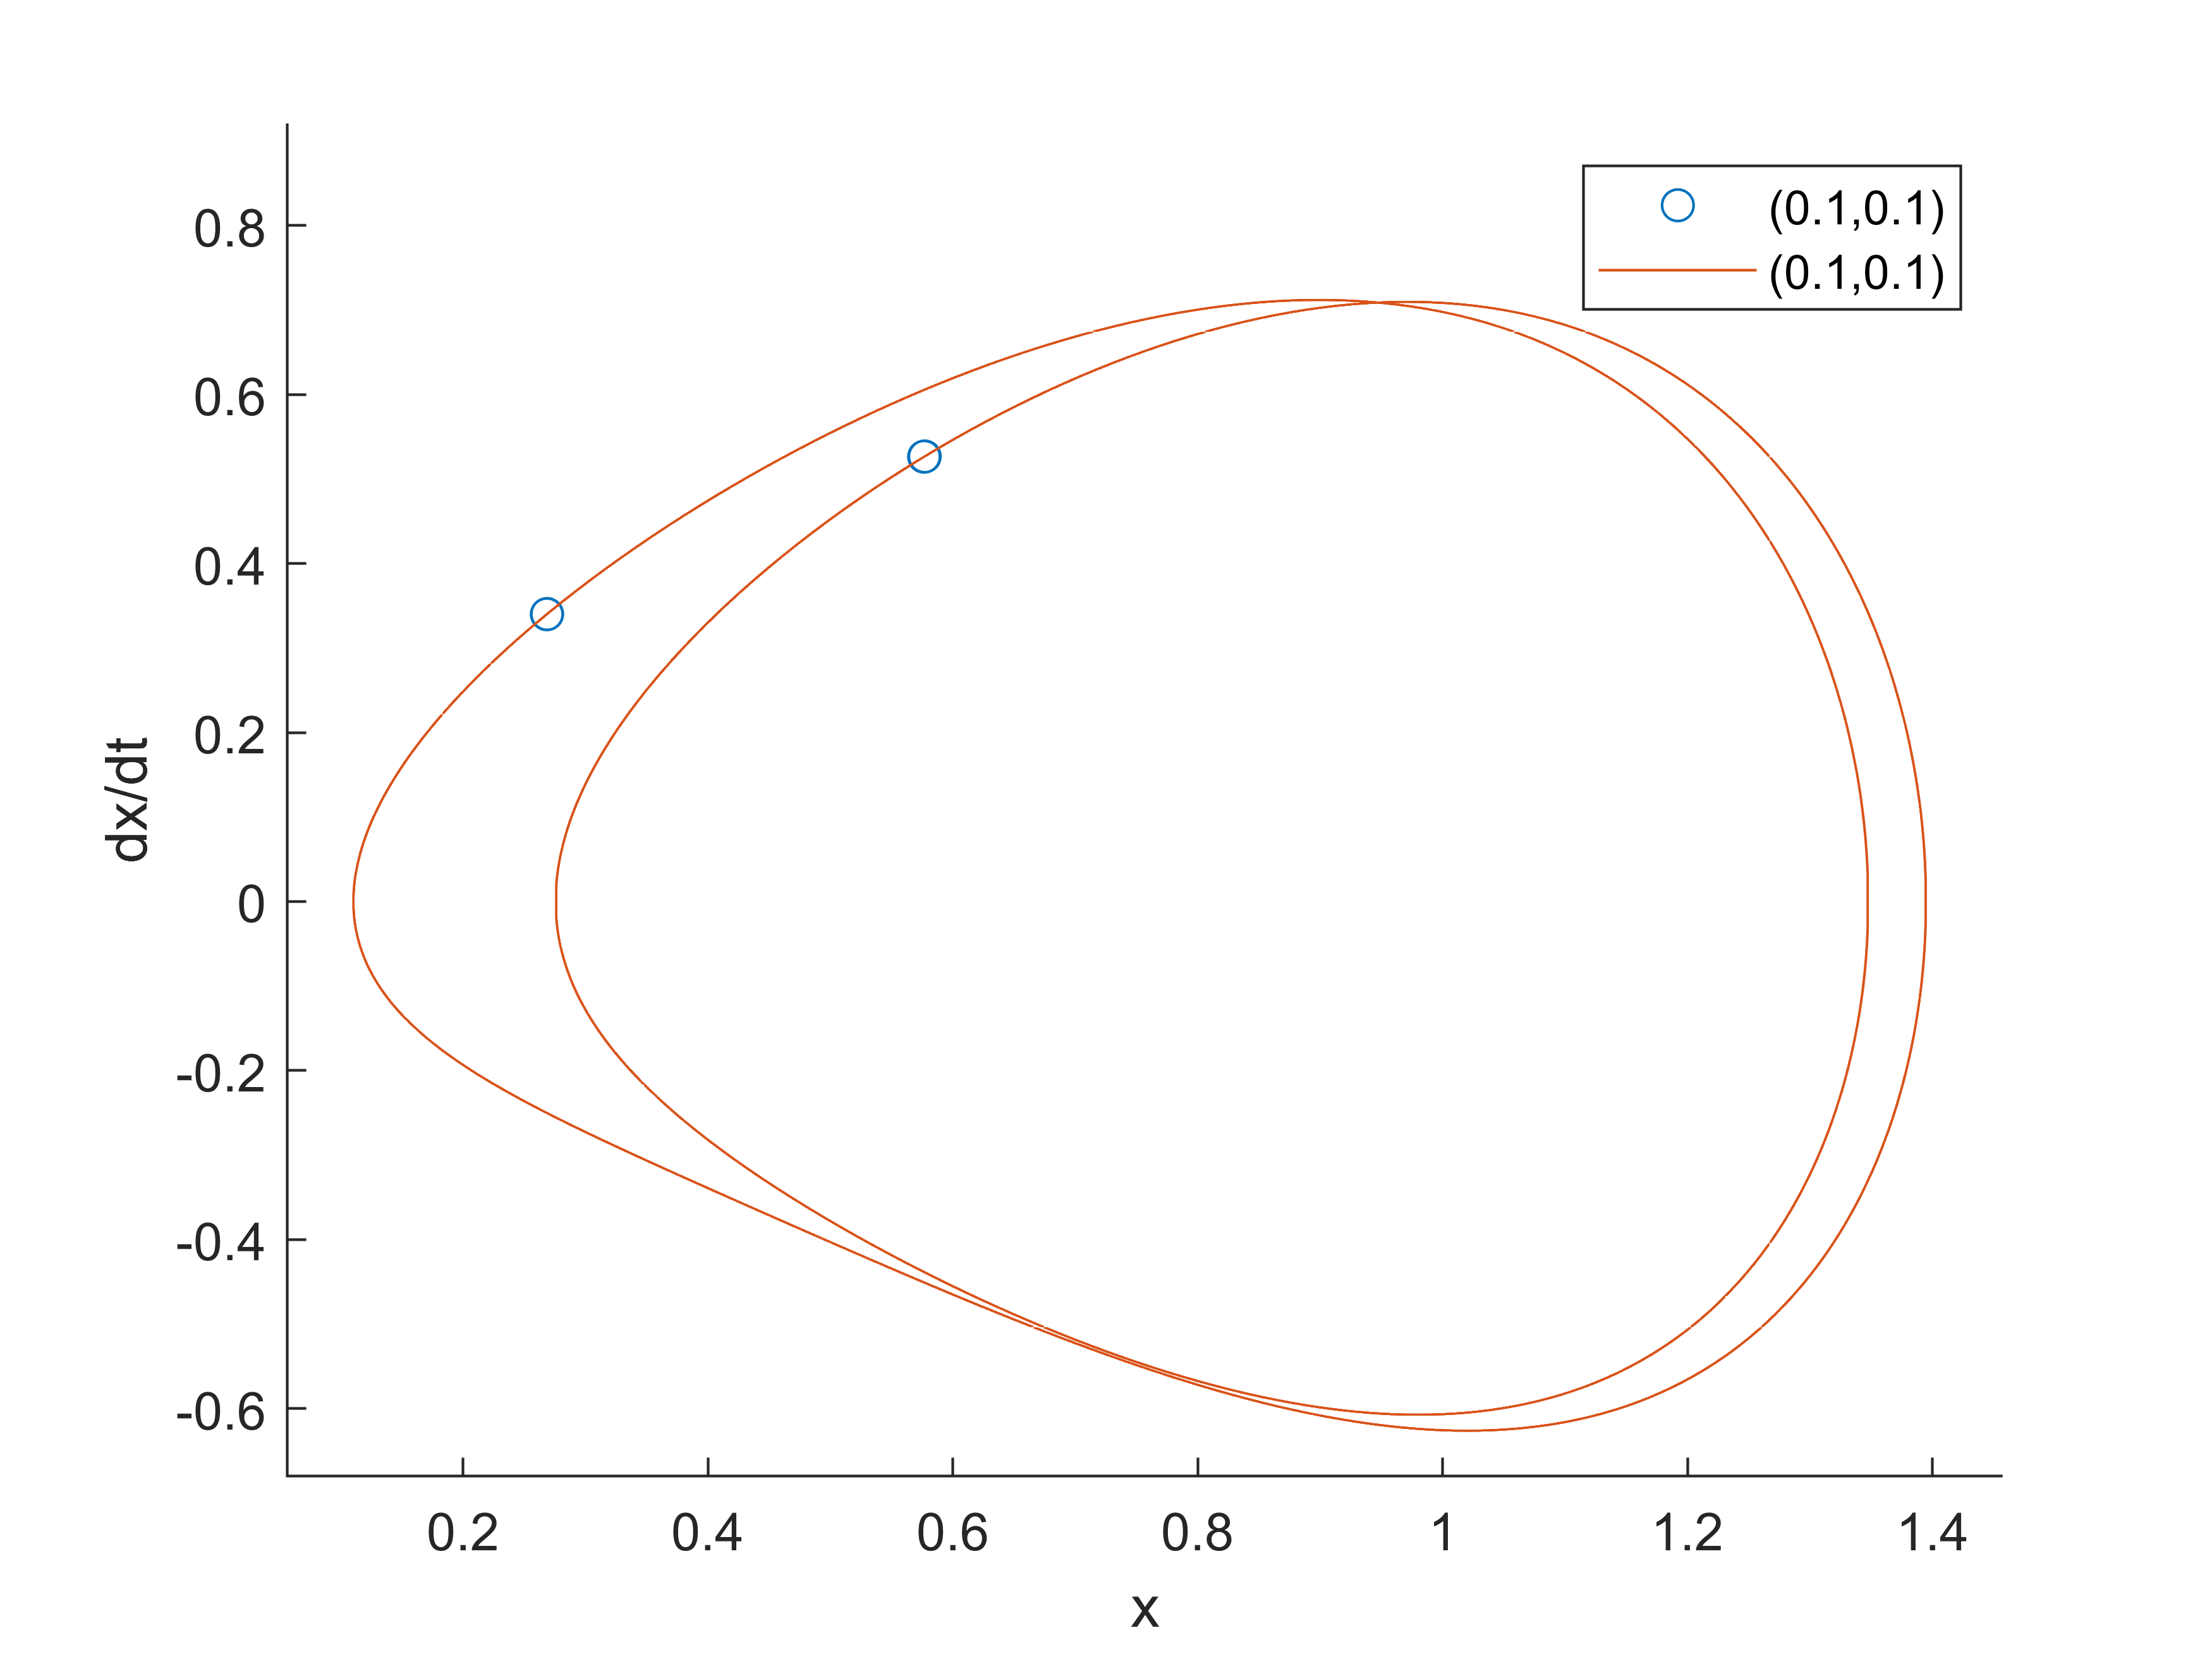
\includegraphics[width=\textwidth]{Files/q5,a=0.423.png}
            \caption{Graph of periodic orbits on x(t) against $\dot{x}(t)$ for $a=0.423$}
        \end{minipage}
\end{figure}
\begin{figure}[H]
    \begin{minipage}[b]{0.5\linewidth}
            \centering
            \textbf{a=0.4178}\par
            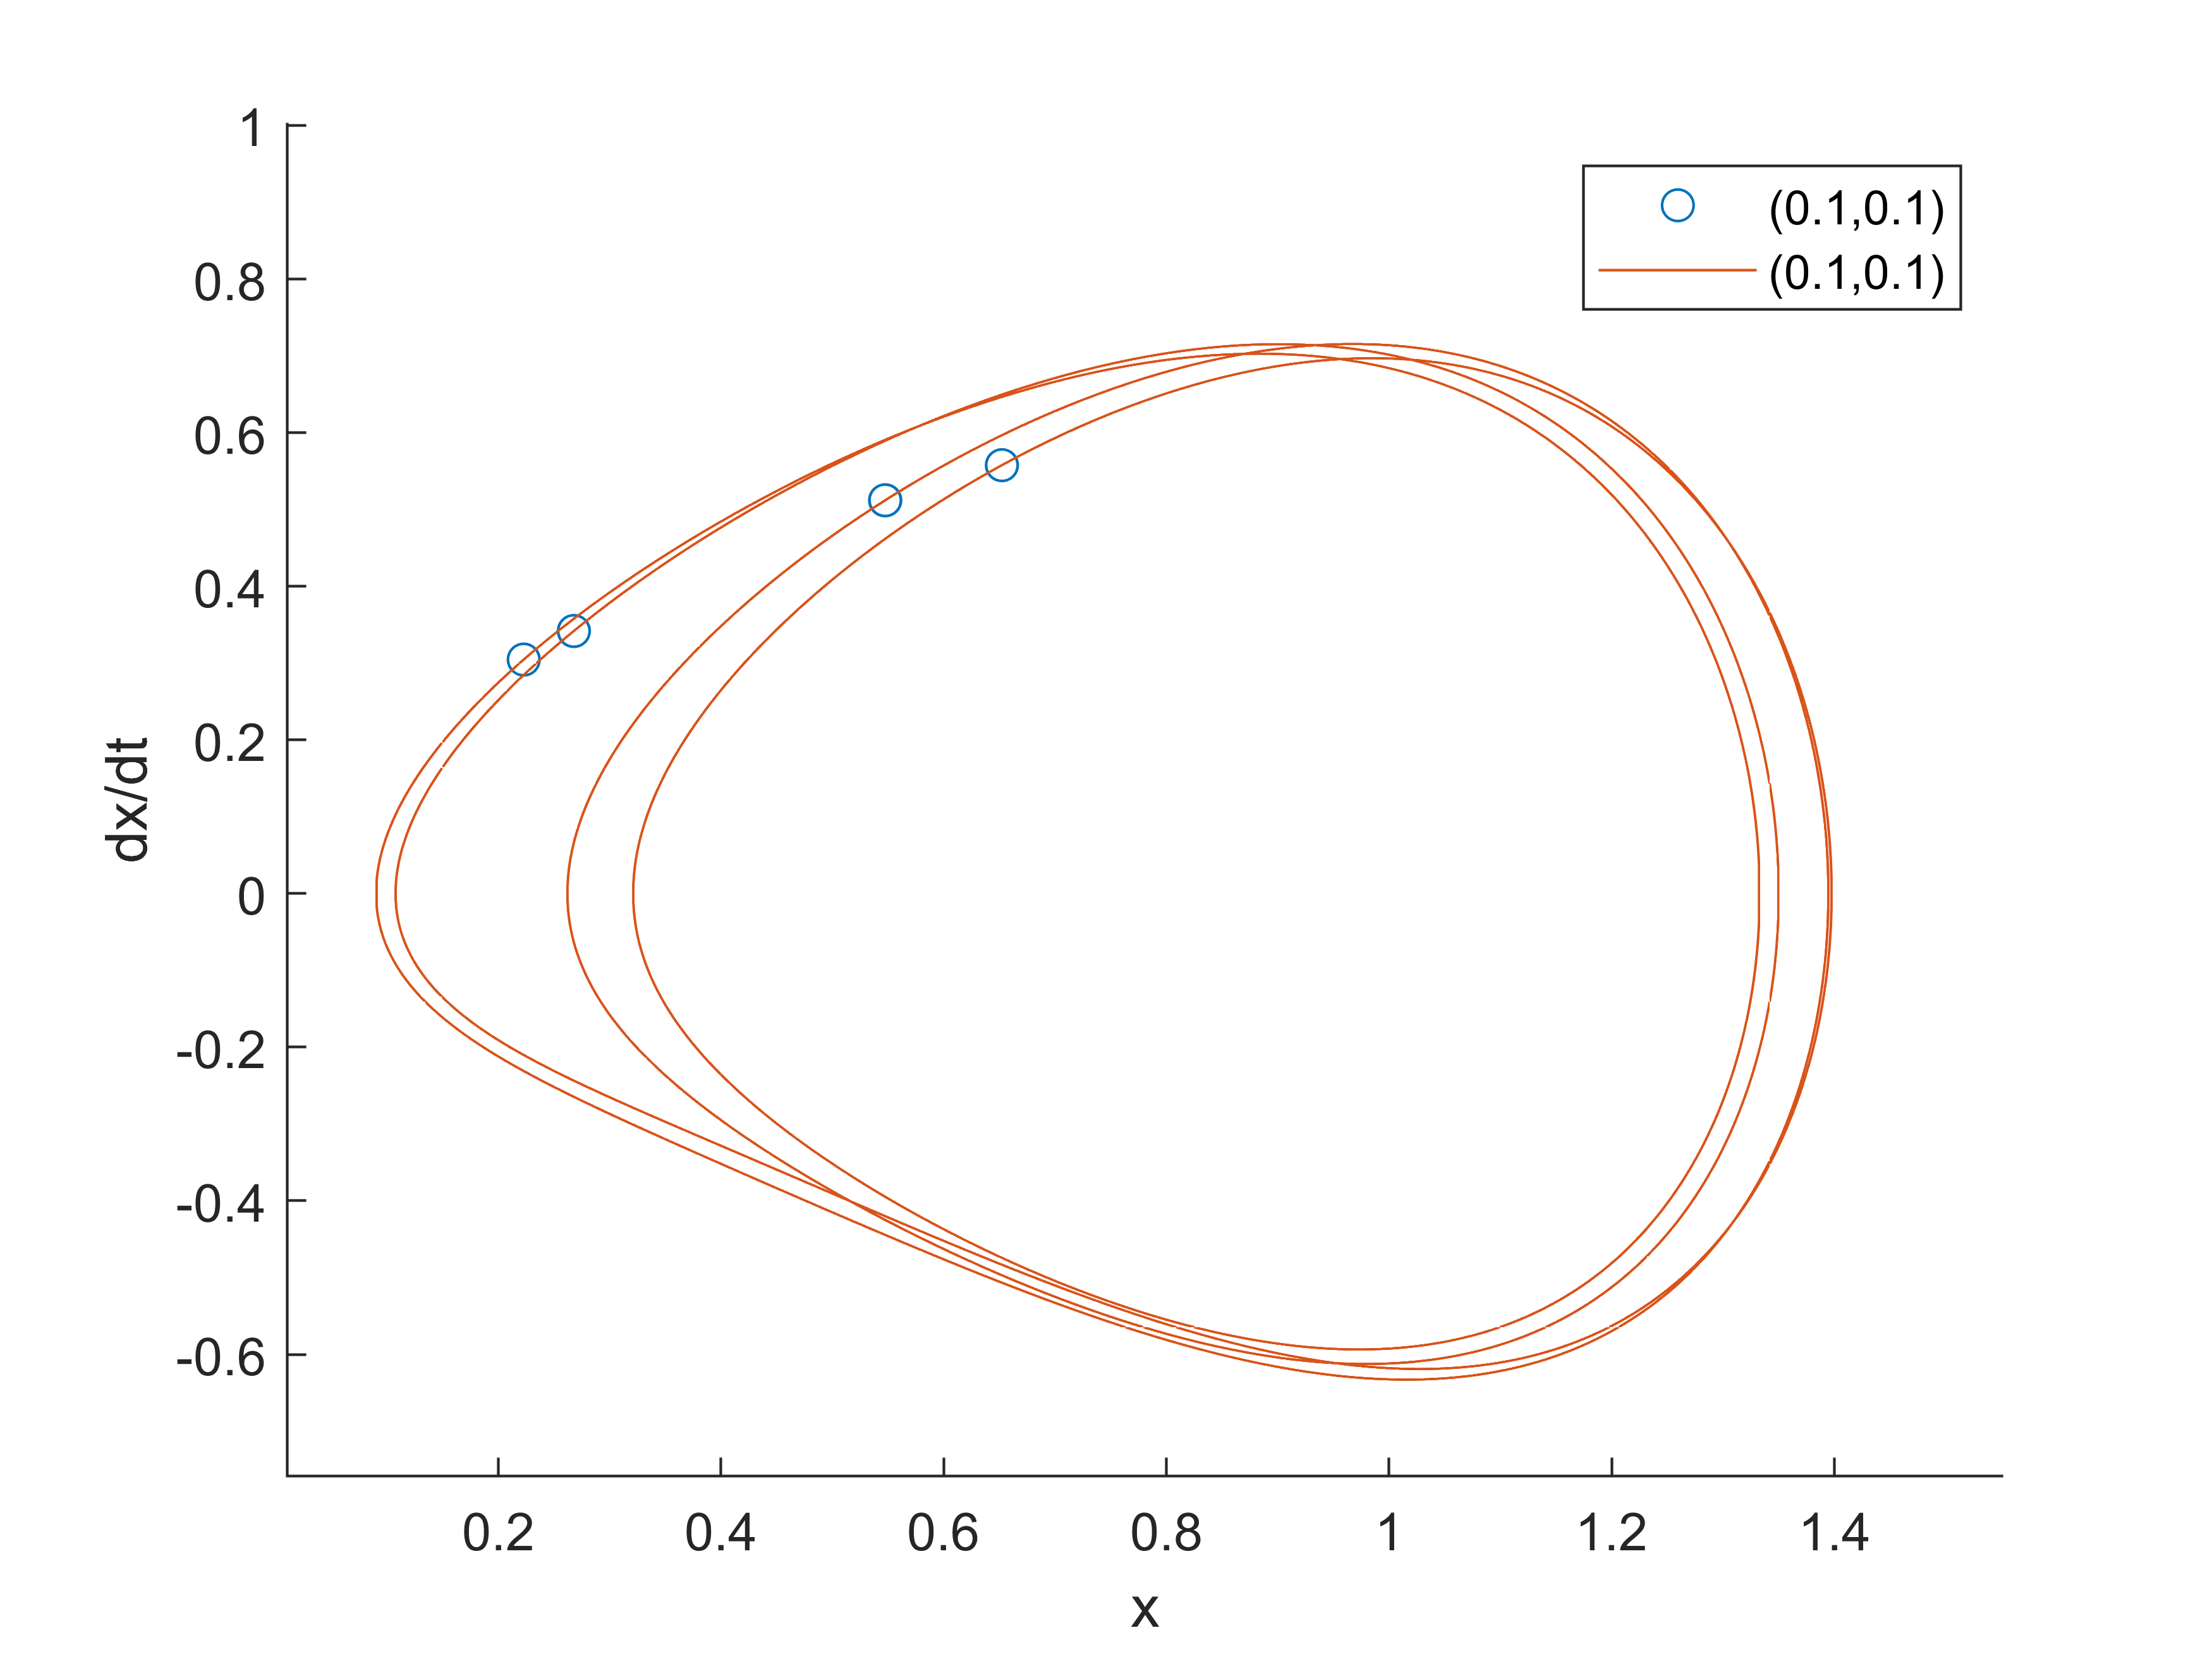
\includegraphics[width=\textwidth]{Files/q5,a=0.4178.png}
            \caption{Graph of periodic orbits on x(t) against $\dot{x}(t)$ for $a=0.4178$}
        \end{minipage}
        \hfill
        \begin{minipage}[b]{0.5\linewidth}
            \centering
            \textbf{a=0.23}\par
            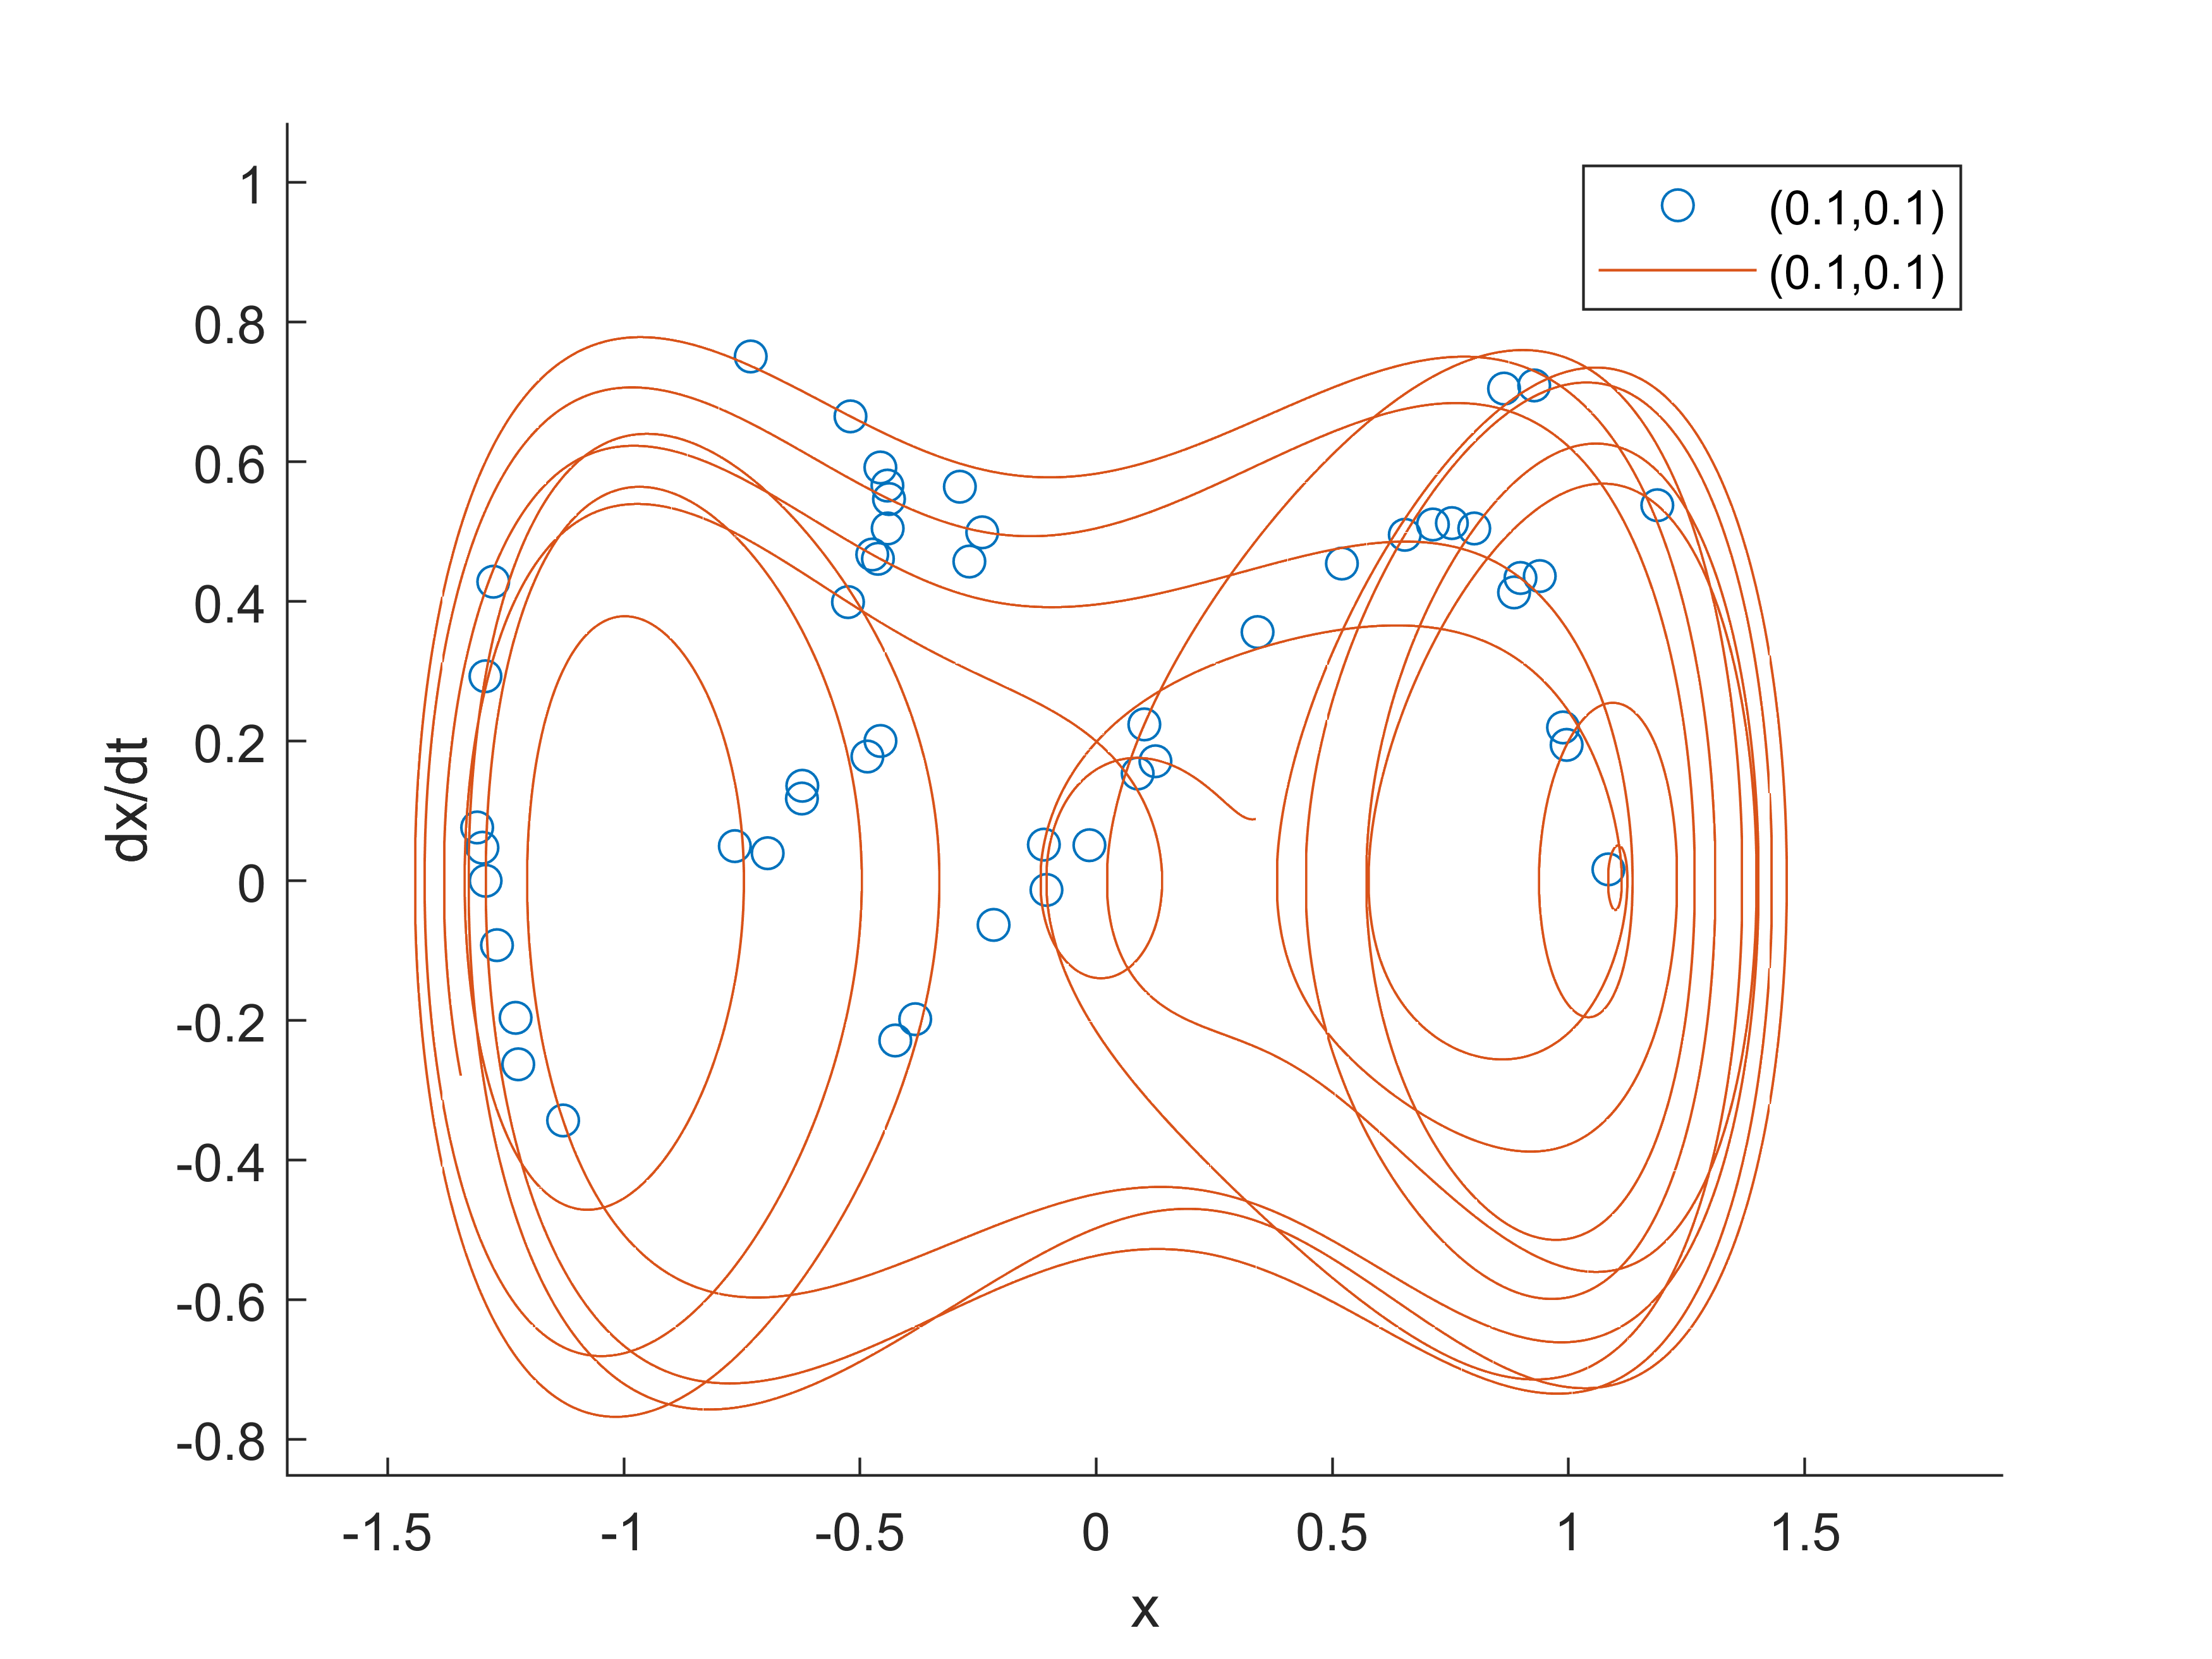
\includegraphics[width=\textwidth]{Files/q5,a=0.23.png}
            \caption{Graph of periodic orbits on x(t) against $\dot{x}(t)$ for $a=0.23$}
        \end{minipage}
\end{figure}
\begin{figure}[H]
\centering
\textbf{a=0.22}\par
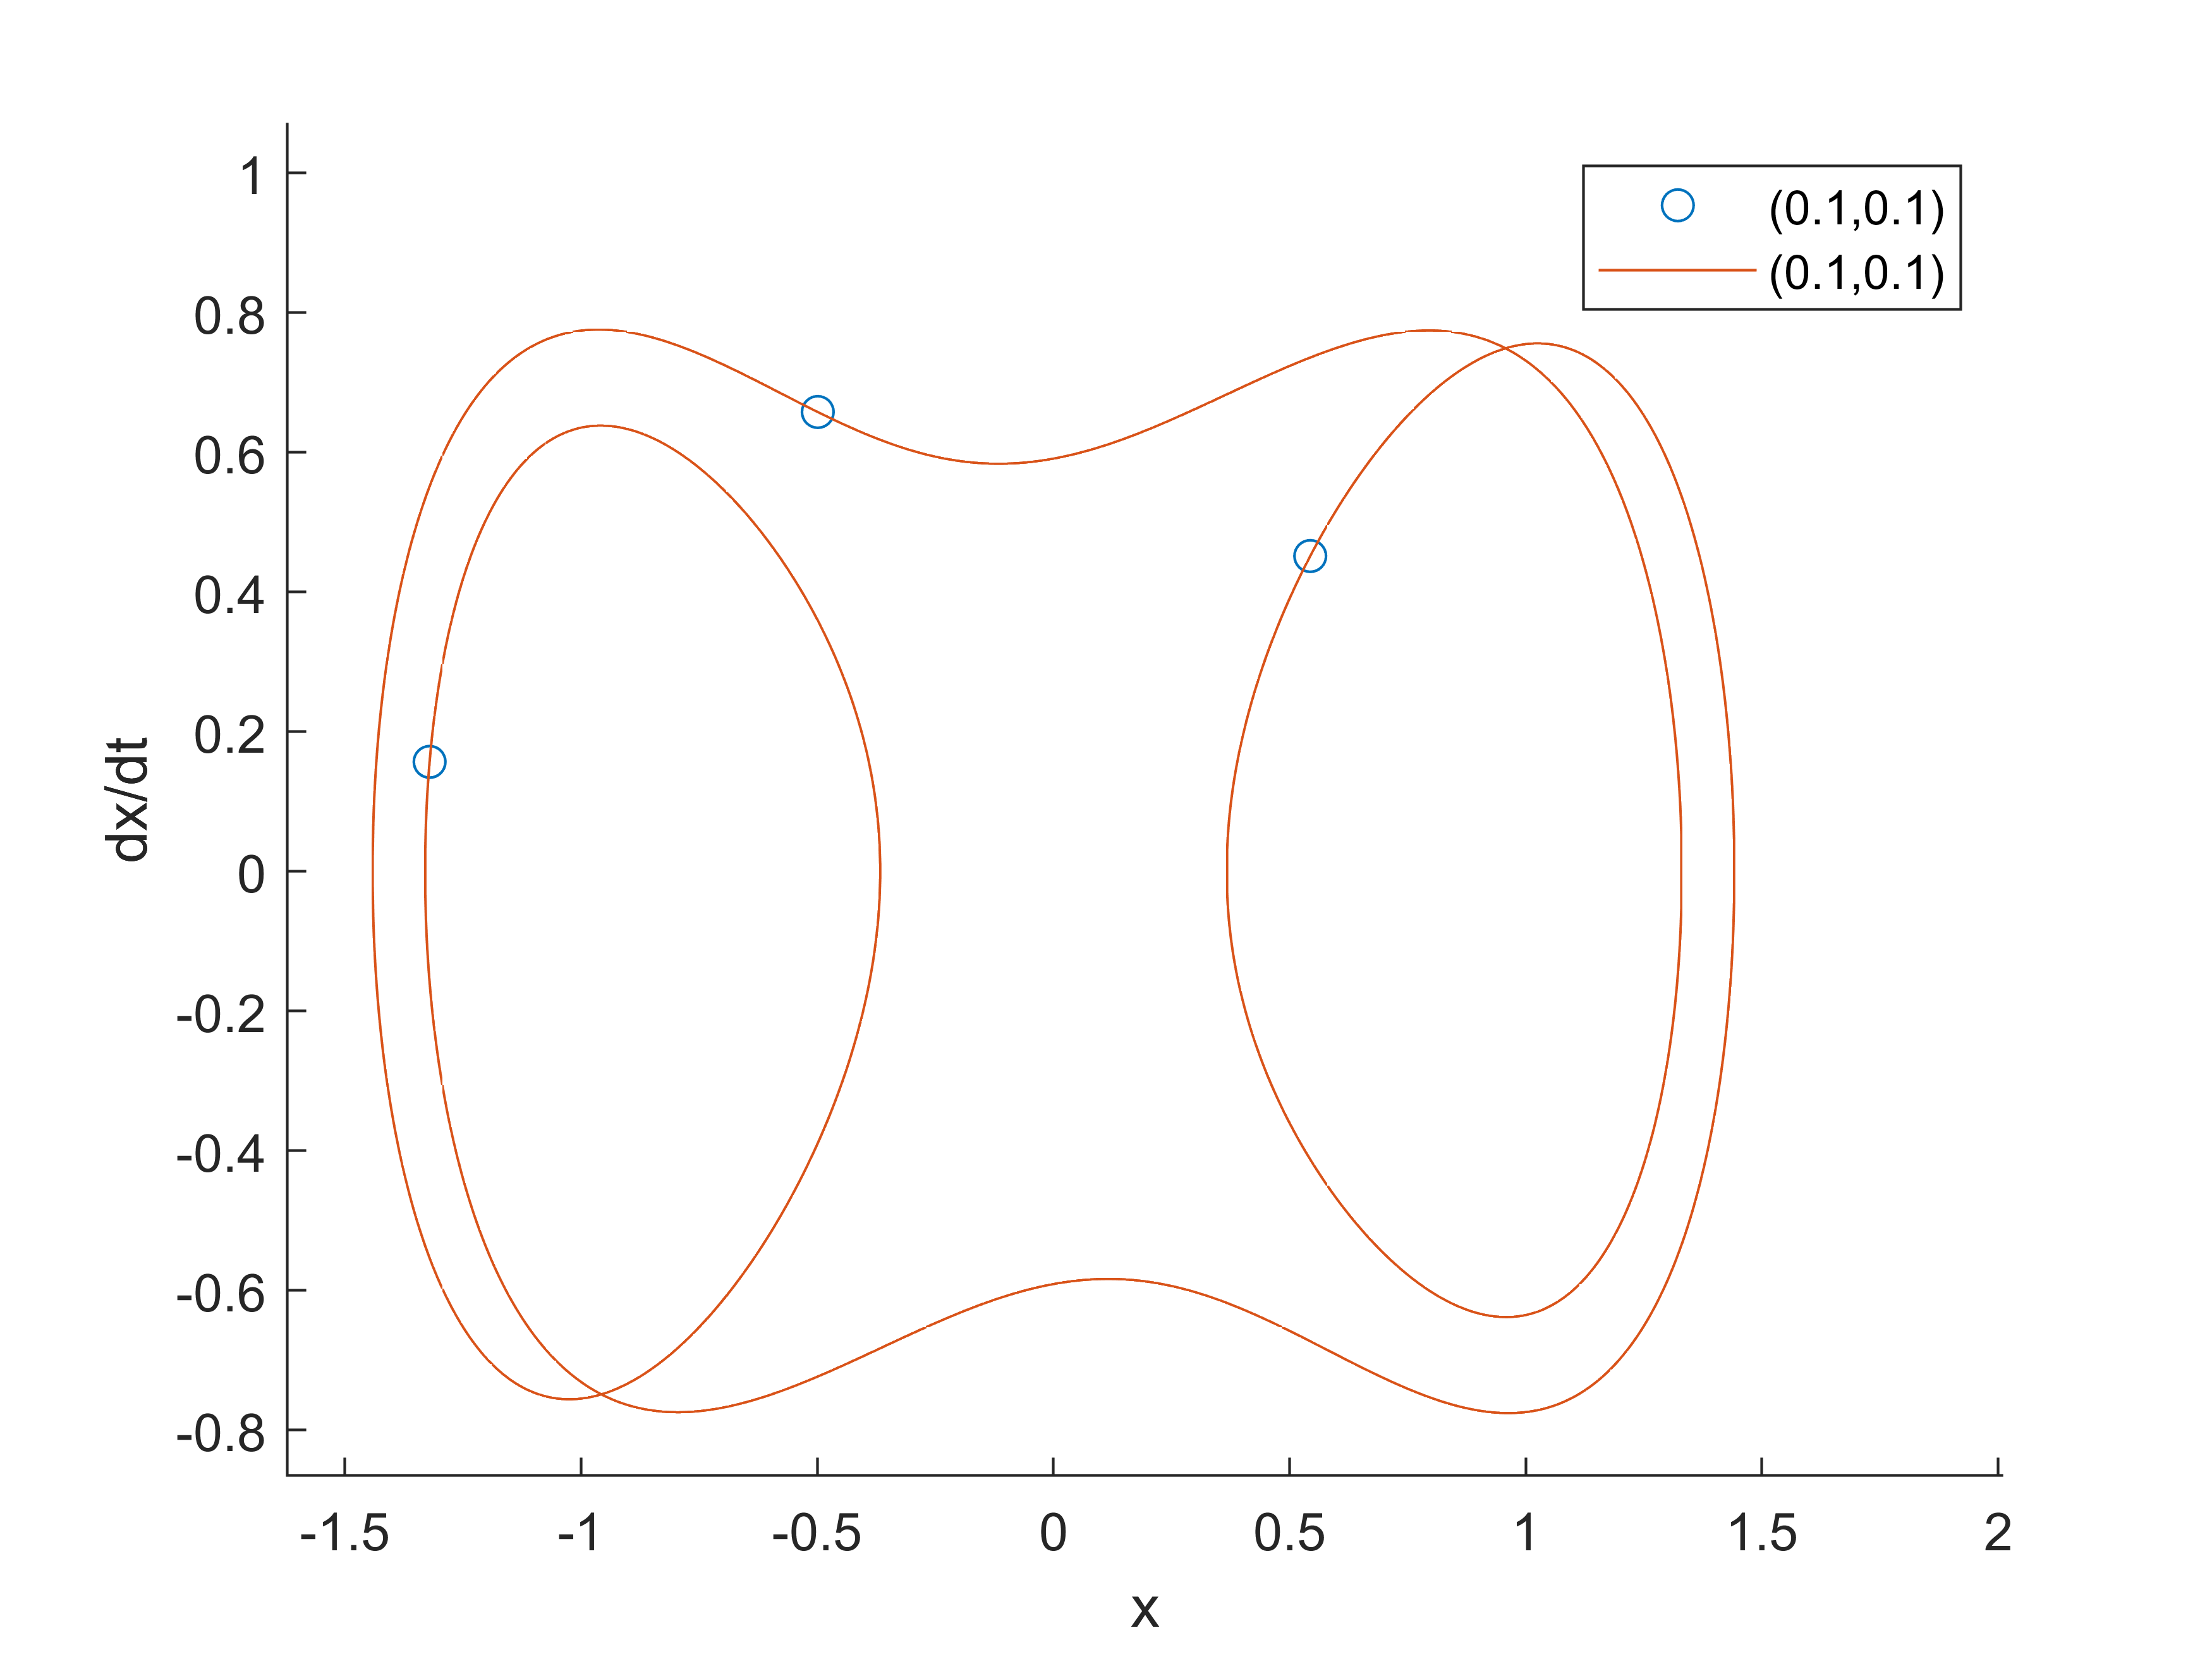
\includegraphics[width=0.45\textwidth]{Files/q5,a=0.22.png}
\caption{Graph of periodic orbits on x(t) against $\dot{x}(t)$ for $a=0.22$}
\end{figure}
\noindent In figure 7, $a=0.44$, we can clearly see only one periodic orbit with period $2\pi$, as there is only one point plotted on the orbit. This shows that it has period $2\pi$.\\
In figure 8, $a=0.423$, there is now two points plotted on the orbit and the trajectory goes around $(-1,0)$ twice rather than once as in figure 7. This shows that it has period $4\pi$.\\
In figure 9, $a=0.4178$, the orbit goes around $(-1,0)$ four times and four corresponding points are plotted on the orbit. This shows that it has period $8\pi$.\\
In figure 10, $a=0.23$, the orbit is totally chaotic, and there is no periodic orbit and the points at $t=2n\pi$ are randomly distributed.\\
In figure 11, $a=0.22$, the orbit goes around $(1,0)$ and $(-1,0)$ once each and around both once. Hence, it has period $6\pi$.\\
We note going from $a=0.4178$ to $a=0.23$, the shape of the solutions are different, when $a$ large, the solution only goes around $(1,0)$. But as $a$ decreases, the solution also traverses where $x<0$ and around $(-1,0)$. Initially, the solution is chaotic as in $a=0.23$, but it settles down a differently shaped periodic orbit as $a$ reaches $0.22$, then solution becomes chaotic again as $a$ gets smaller than $0.21$.

\newpage
\section*{Part 2}
\subsection*{Question 6}
Let $\dot{x}=y$, then the equation becomes 
\[\left
\{\begin{array}{lr}
\dot{x}=y\\
\dot{y}=ax-x^3+(b-x^2)y
\end{array}
\right.\]
The points I've chosen in the different regions are:
\begin{flalign*}
 &(a,b)=\left
\{\begin{array}{lr}
(-1,-1)&\quad\text{Region 1;}\\
(-1,1)&\text{Region 2;}\\
(0.7,1)&\text{Region 3;}\\
(\frac{9}{8},1)&\text{Region 4;}\\
(1.28,1)&\text{Region 5;}\\
(1.5,1)&\text{Region 6.}
\end{array}
\right.&
\end{flalign*}
The program used to plot the graphs below can be found in the programs section under the title \emph{'vi) q6.m'}. The different initial conditions used can be found in the legend of each figure.
\begin{figure}[H]
    \begin{minipage}[b]{0.5\linewidth}
            \centering
            \textbf{Region 1}\par
            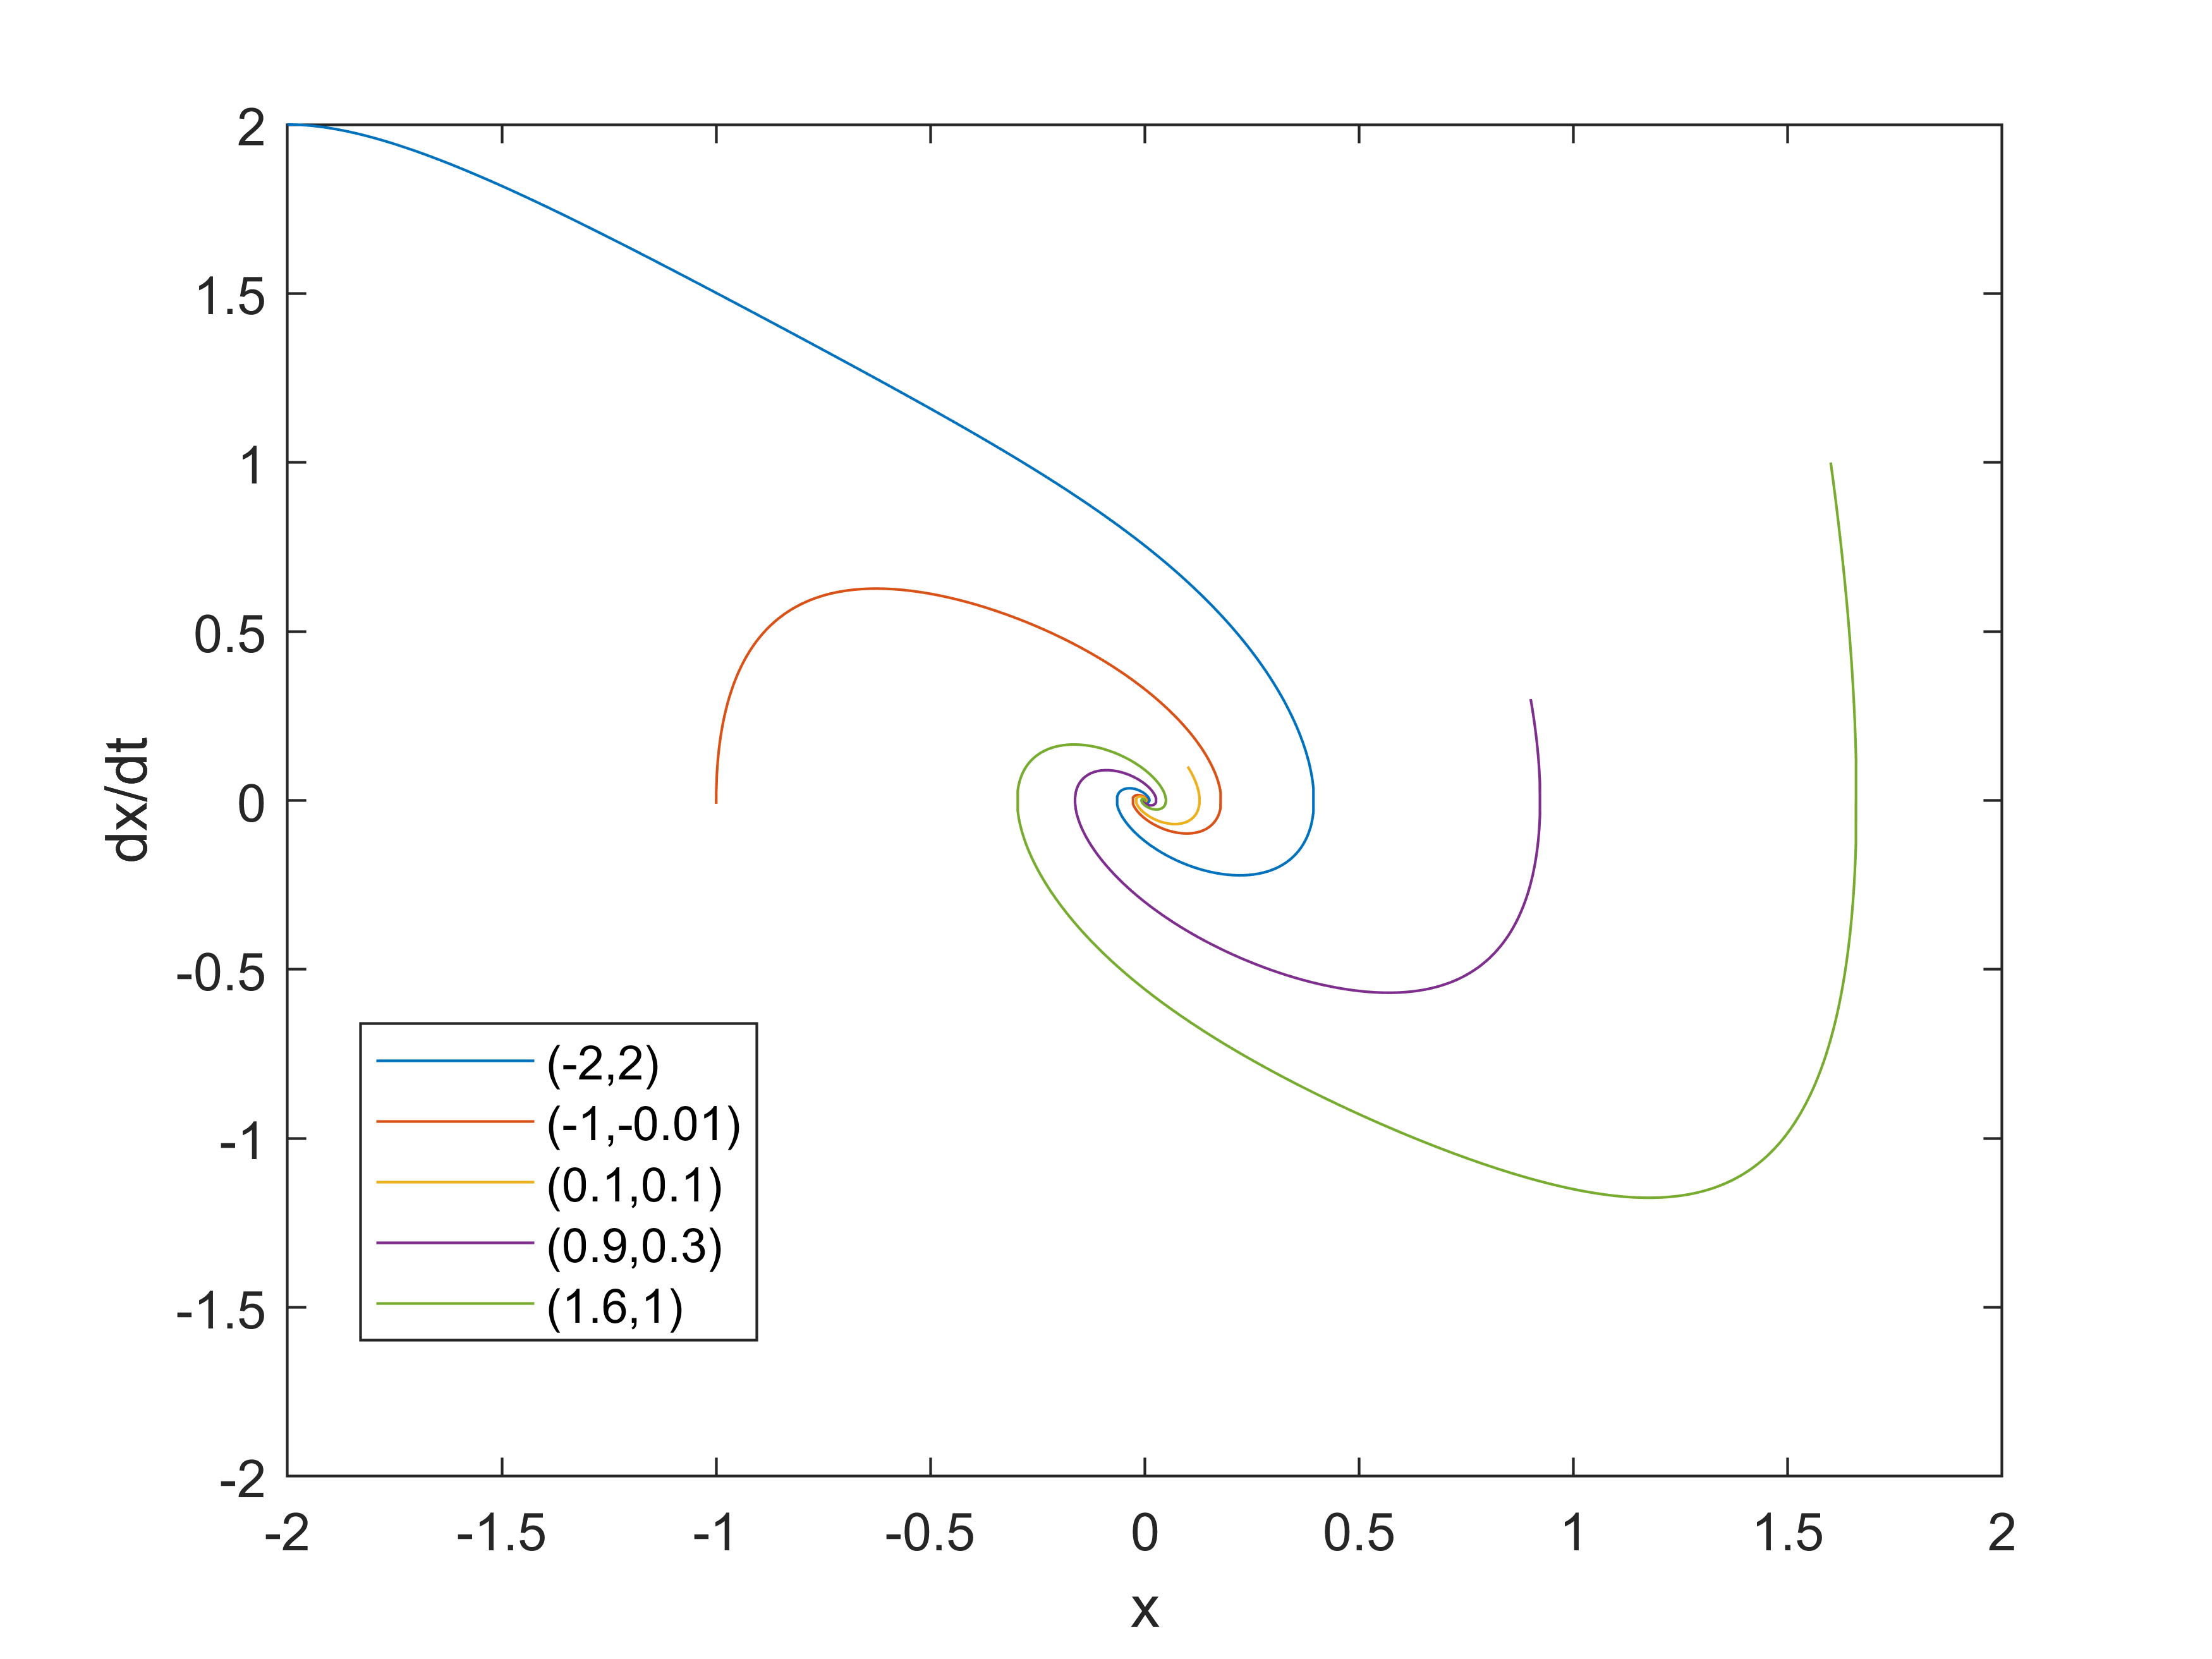
\includegraphics[width=\textwidth]{Files/q6,region1.png}
            \caption{Graph of x(t) against $\dot{x}(t)$ with $(a,b)=(-1,-1)$}
        \end{minipage}
        \hfill
        \begin{minipage}[b]{0.5\linewidth}
            \centering
            \textbf{Region 2}\par
            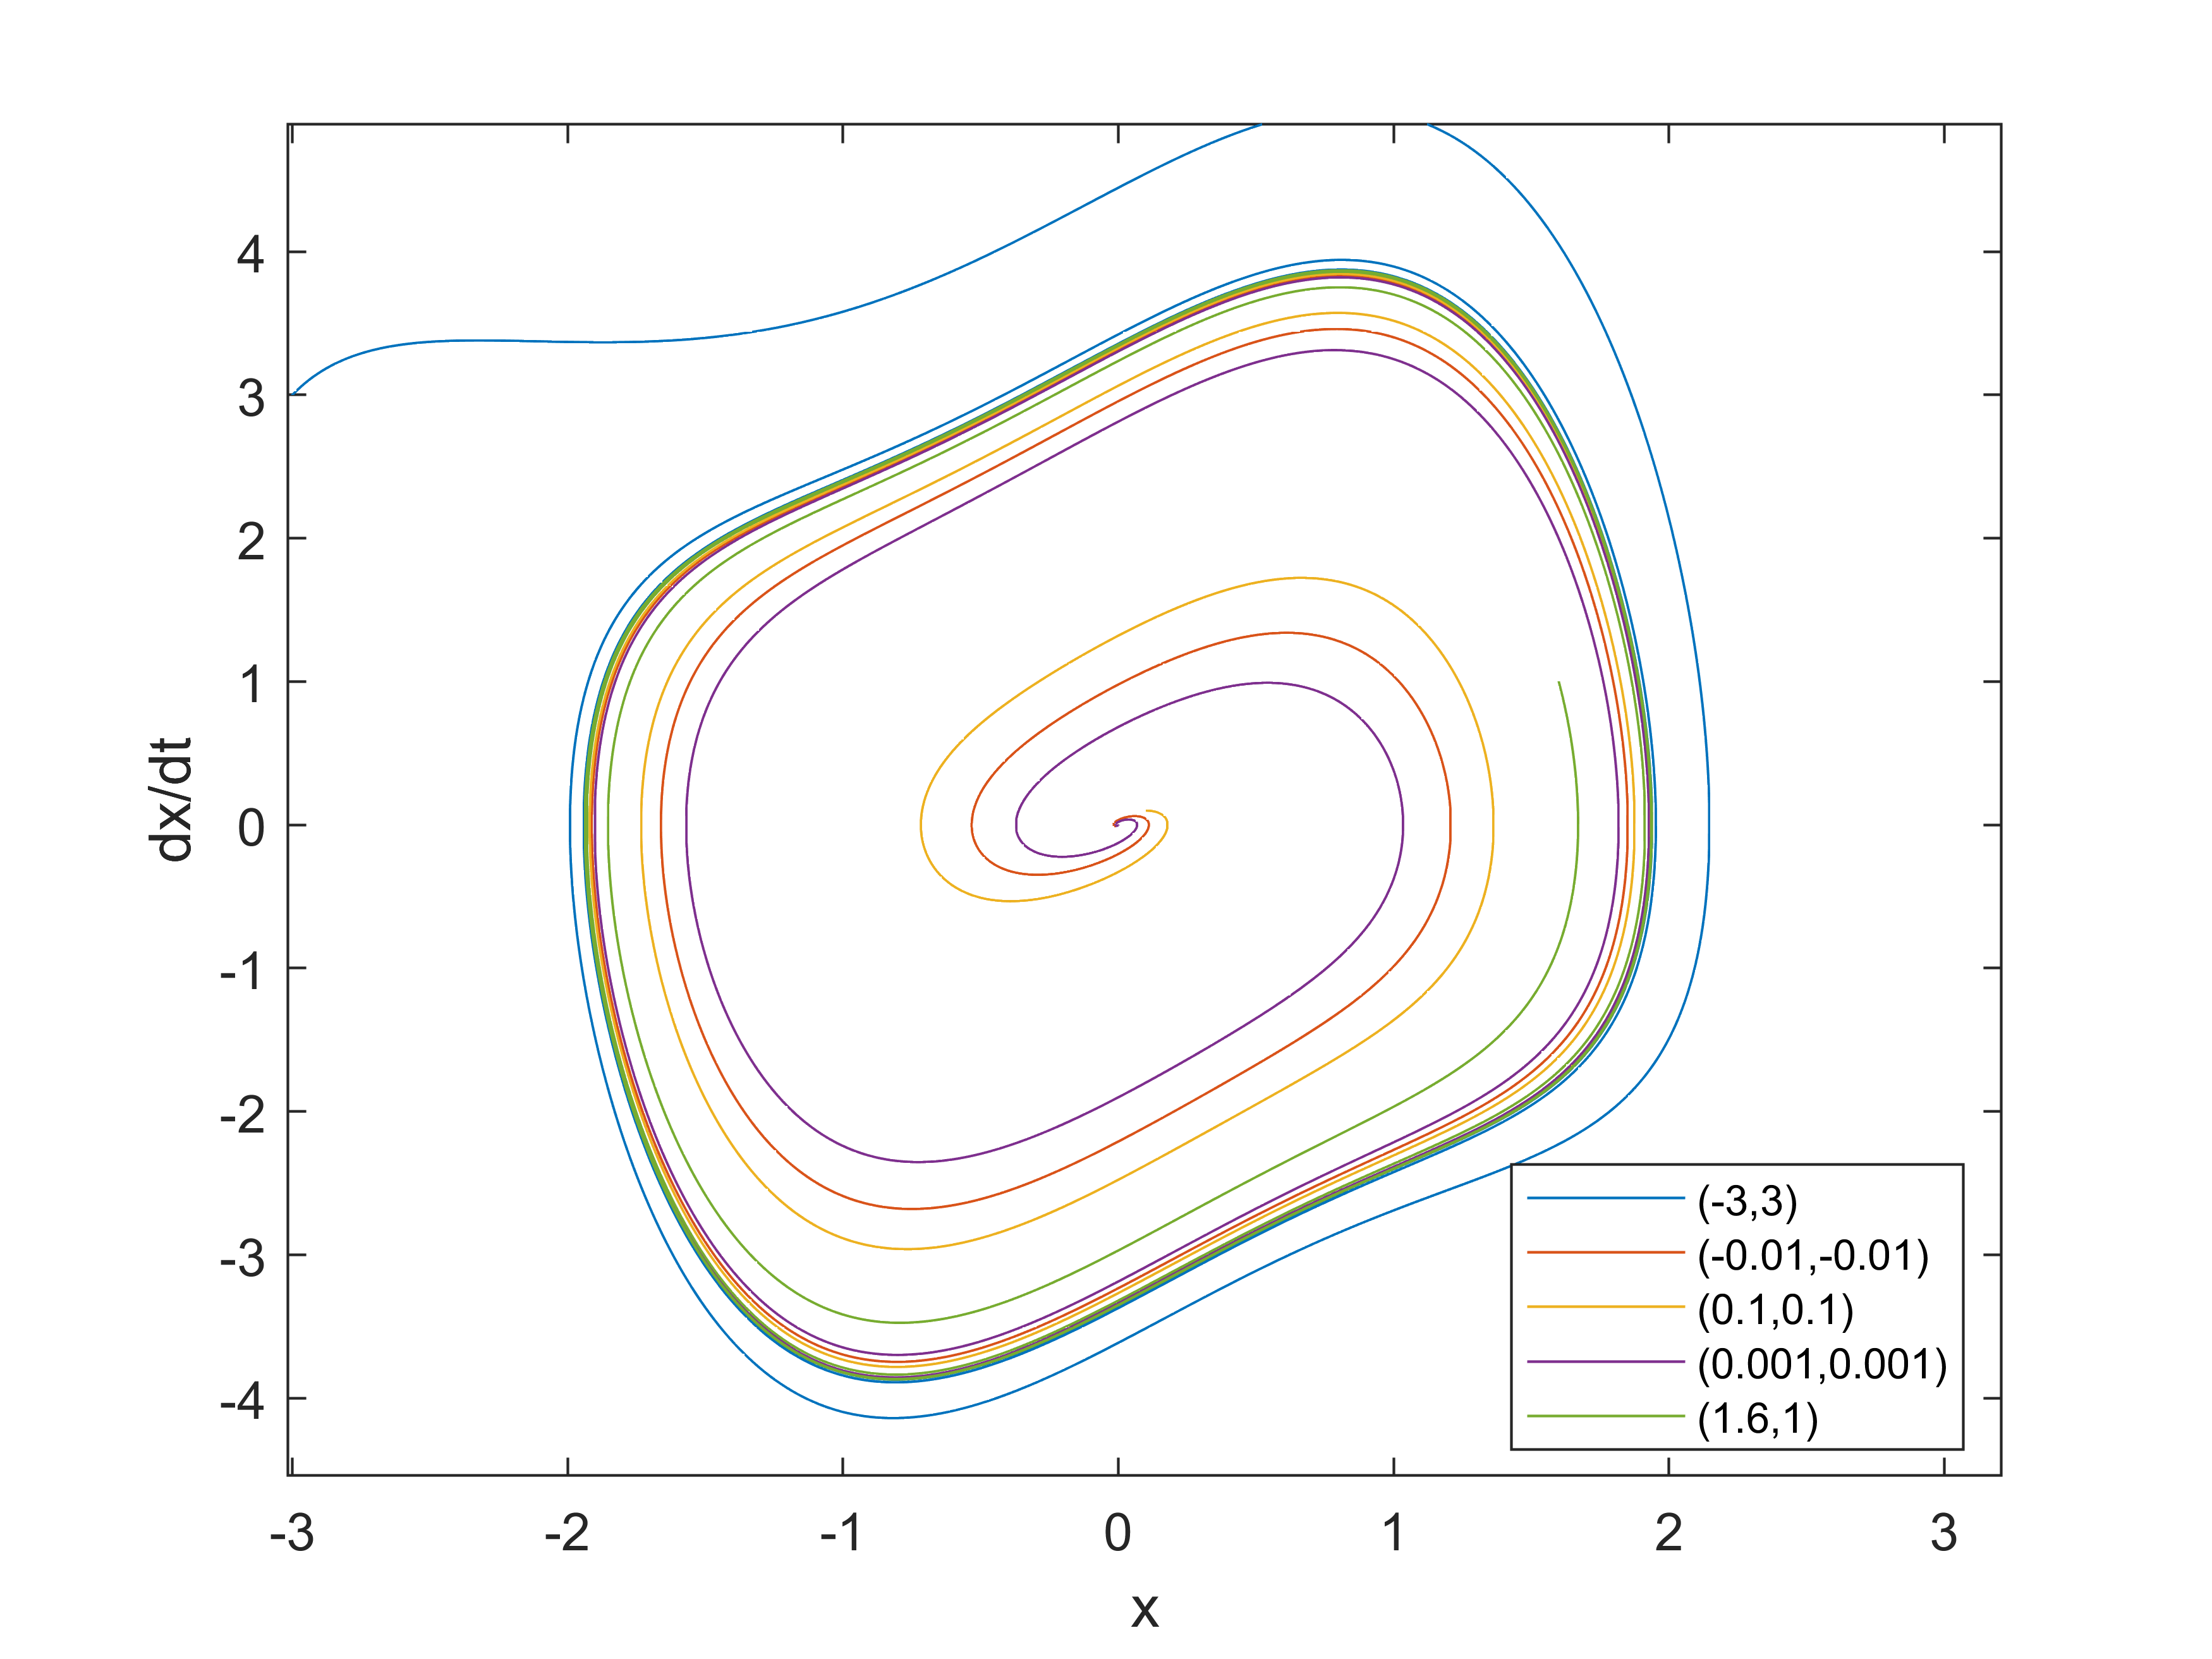
\includegraphics[width=\textwidth]{Files/q6,region2.png}
            \caption{Graph of x(t) against $\dot{x}(t)$ with $(a,b)=(-1,1)$}
        \end{minipage}
\end{figure}
\noindent In figure for region 1, there's one fixed point at $(0,0)$ which is a stable focus and global attractor. The trajectories plotted all eventually tend towards it.\\
In figure for region 2, there's one fixed point at $(0,0)$, which is a unstable focus, so trajectories with initial conditions near $(0,0)$ moves away from it. However, there exists a periodic orbit which these trajectories tend to as well as trajectories with initial conditions outside of the periodic orbit.
\begin{figure}[H]
    \begin{minipage}[b]{0.5\linewidth}
            \centering
            \textbf{Region 3}\par
            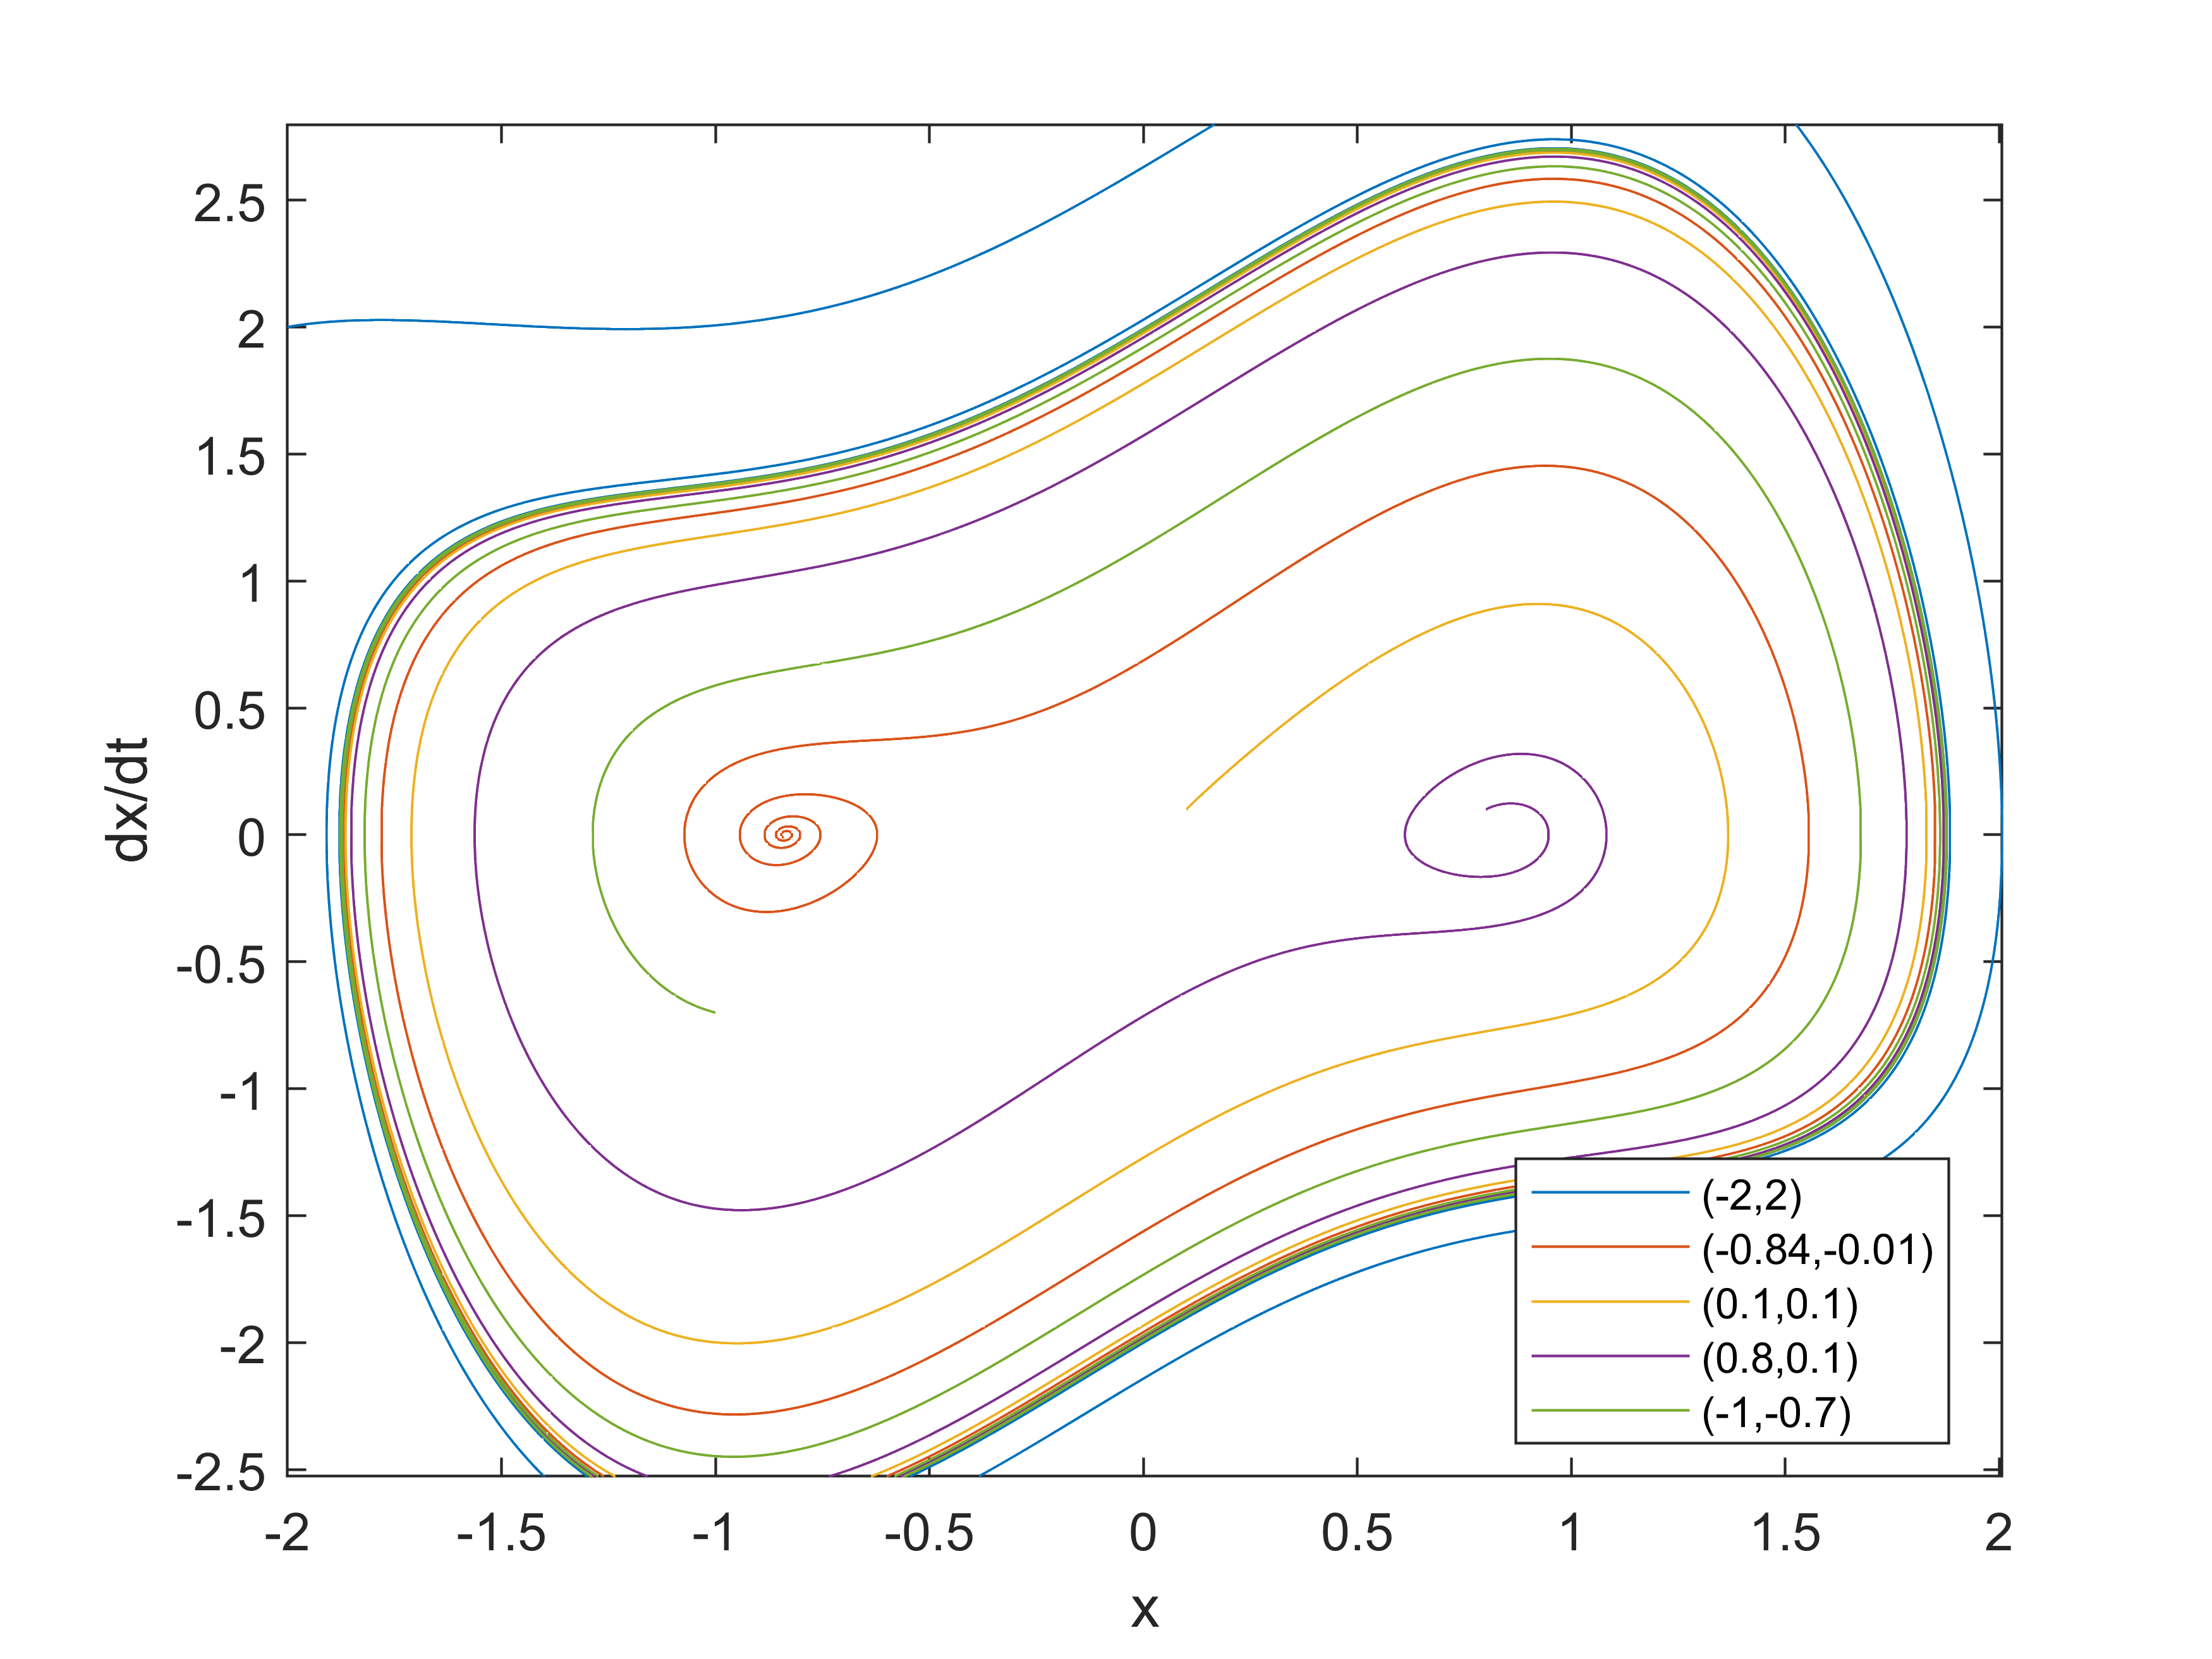
\includegraphics[width=\textwidth]{Files/q6,region3.png}
            \caption{Graph of x(t) against $\dot{x}(t)$ with $(a,b)=(0.7,1)$}
        \end{minipage}
        \hfill
        \begin{minipage}[b]{0.5\linewidth}
            \centering
            \textbf{Region 4}\par
            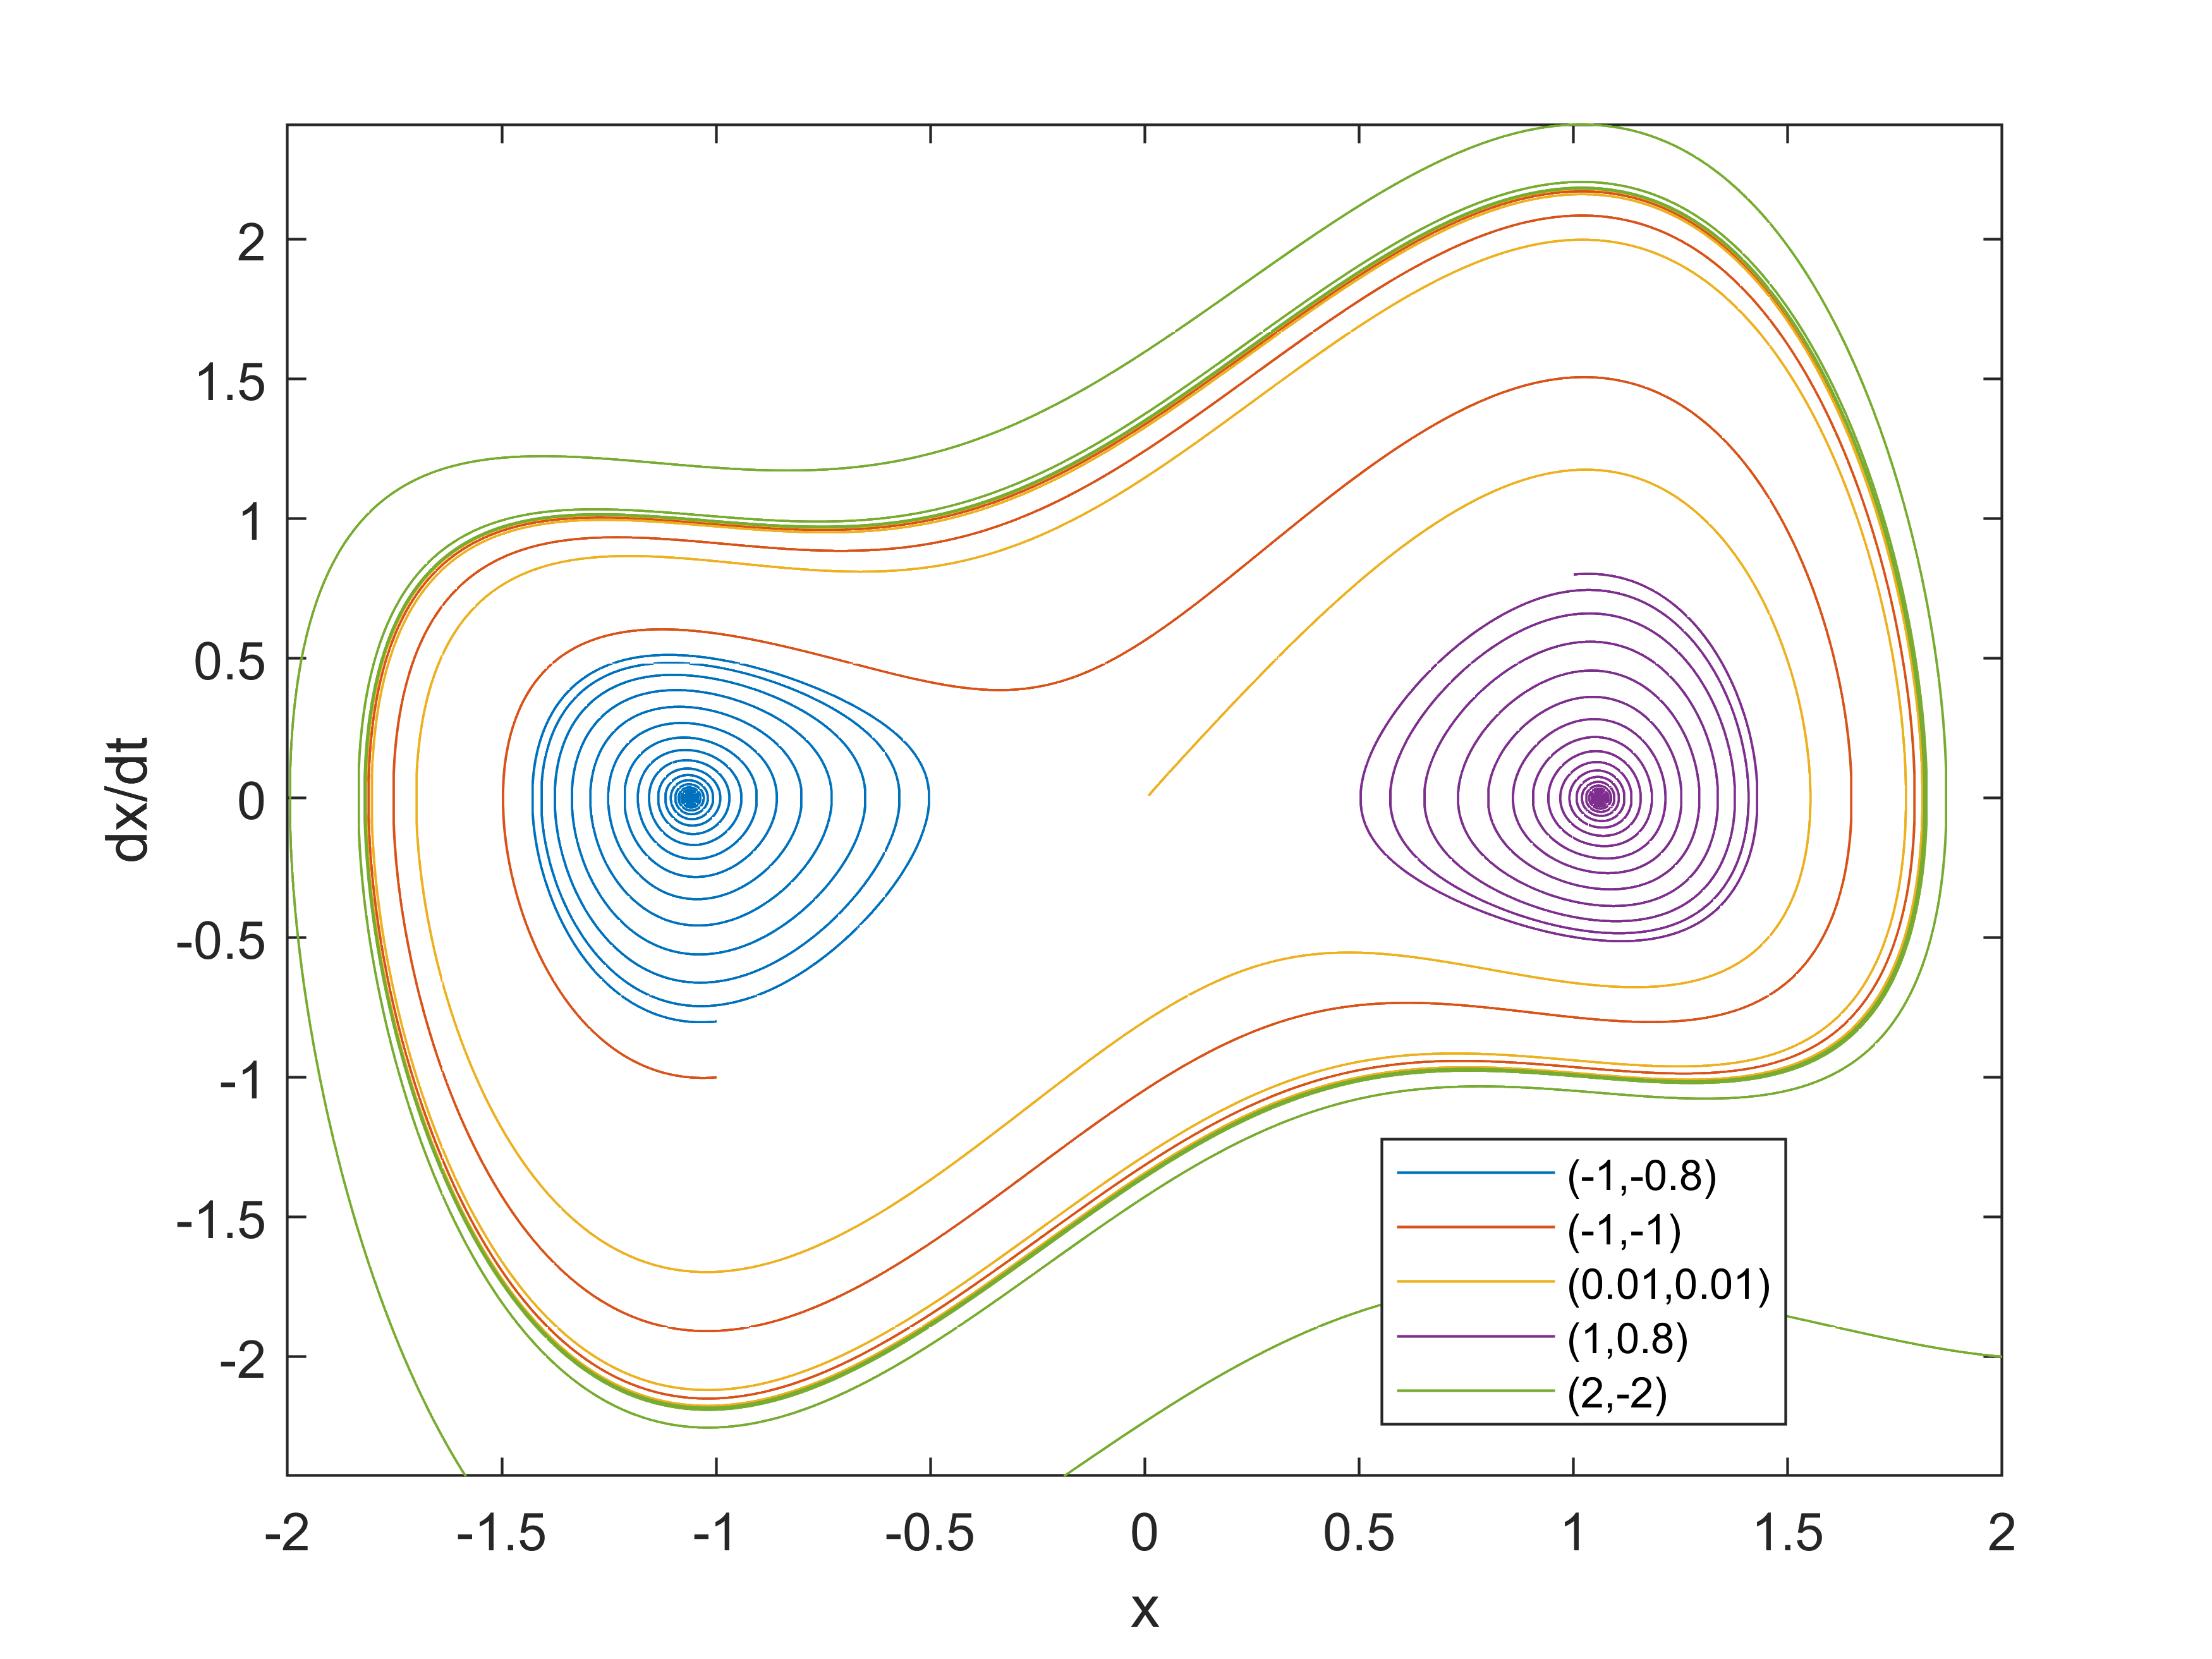
\includegraphics[width=\textwidth]{Files/q6,region4.png}
            \caption{Graph of x(t) against $\dot{x}(t)$ with $(a,b)=(\frac{9}{8},1)$}
        \end{minipage}
\end{figure}
\noindent In figure for region 3, there are three fixed points at $(0,0)$ and $(\pm\sqrt{0.7},0)$. $(0,0)$ is a saddle point and $(\pm\sqrt{0.7},0)$ are unstable foci. The trajectories with initial conditions near these fixed points move away from them and tend to a stable periodic orbit.\\
In figure for region 4, there are three fixed points at $(0,0)$ and $(\pm\sqrt{0.7},0)$. $(0,0)$ is a saddle point and $(\pm\sqrt{0.7},0)$ are stable foci. We note when we start from $(-1,-0.5)$ or $(1,0.5)$, they slowly spiral into the fixed points. However, when we start at $(\pm0.1,\pm0.1)$ or $(-2,2)$, the trajectories tend to the stable periodic orbit outside instead. This implies that we also have two unstable periodic orbits encircling each of the unstable focus.
\begin{figure}[H]
    \begin{minipage}[b]{0.5\linewidth}
            \centering
            \textbf{Region 5}\par
            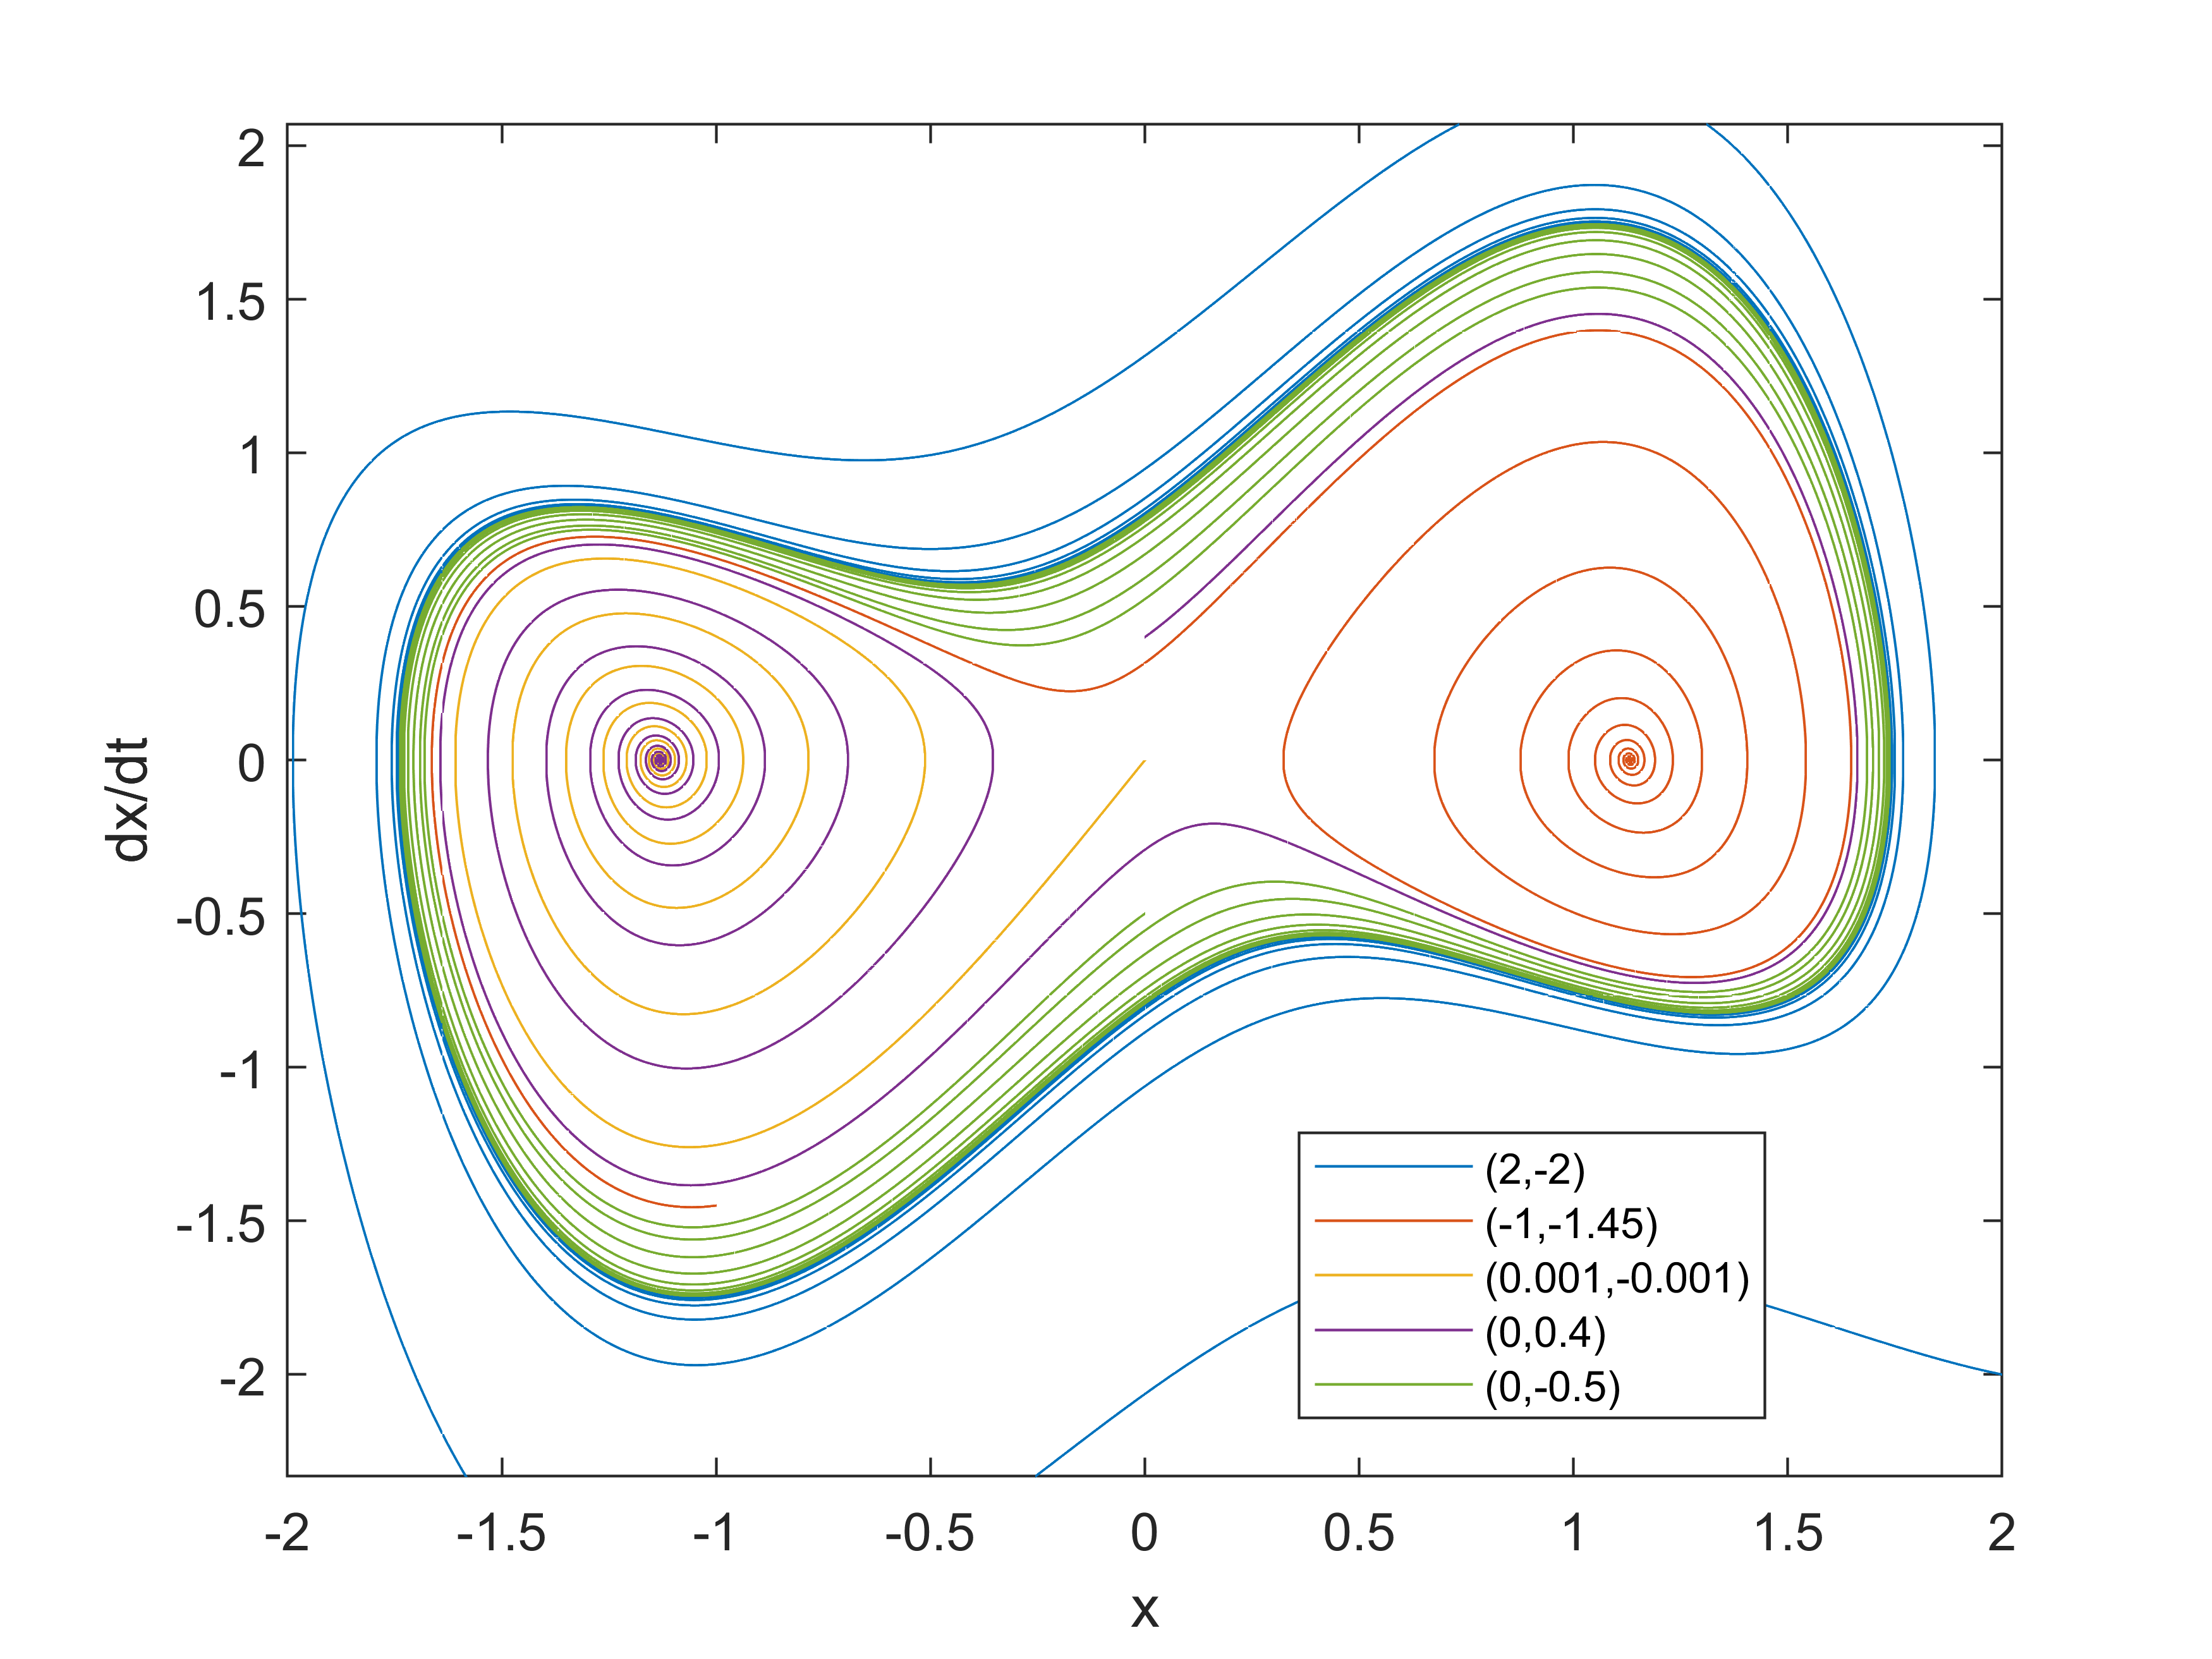
\includegraphics[width=\textwidth]{Files/q6,region5.png}
            \caption{Graph of x(t) against $\dot{x}(t)$ with $(a,b)=(1.28,1)$}
        \end{minipage}
        \hfill
        \begin{minipage}[b]{0.5\linewidth}
            \centering
            \textbf{Region 6}\par
            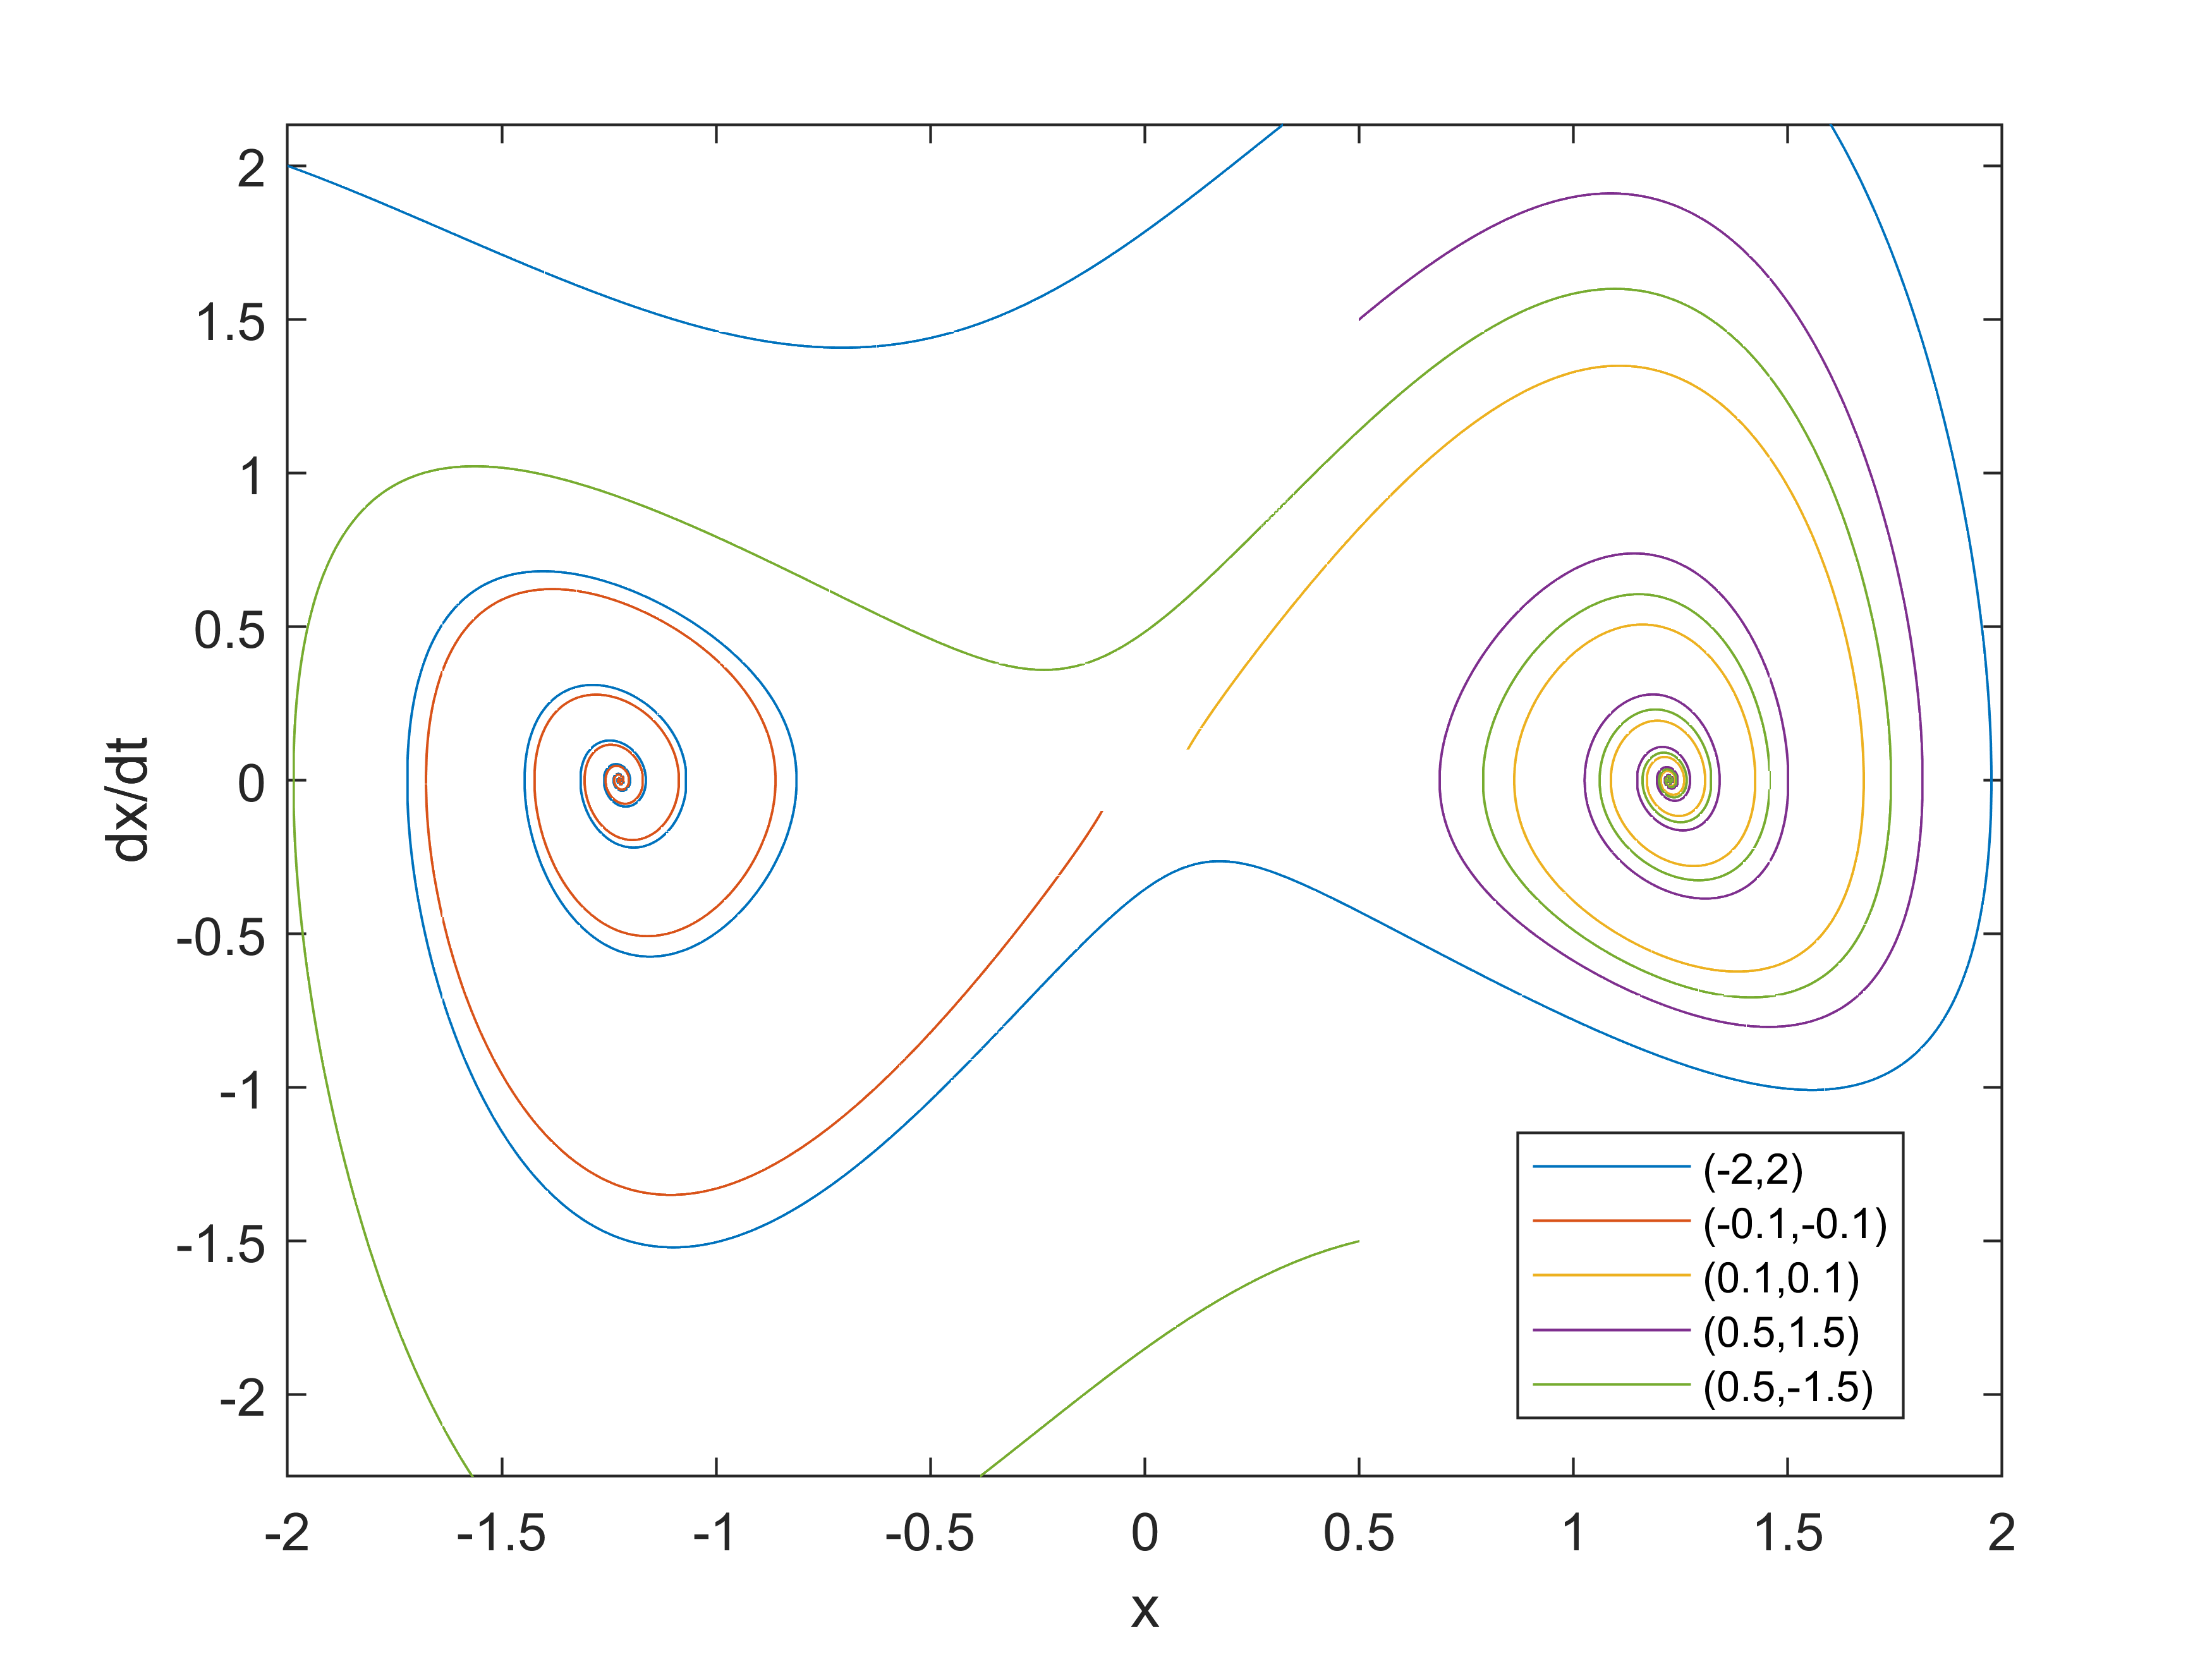
\includegraphics[width=\textwidth]{Files/q6,region6.png}
            \caption{Graph of x(t) against $\dot{x}(t)$ with $(a,b)=(1.5,1)$}
        \end{minipage}
\end{figure}
\noindent For figure in region 5, there are three fixed points at $(0,0)$ and $(\pm\sqrt{0.7},0)$. $(0,0)$ is a saddle point and $(\pm\sqrt{0.7},0)$ are stable foci. This is similar to region 4, but there are two periodic orbits now. The stable periodic orbit which is outside of the unstable periodic orbit. Hence, initial conditions inside the unstable periodic orbit like $(-1,-1,45),(0,0.4)$ would go to the stable fixed points whereas initial conditions between the two periodic orbits will go to the stable one, e.g. $(0,-0.5)$.\\
For figure in region 6, there is no periodic orbit and three fixed points at $(0,0)$ and $(\pm\sqrt{0.7},0)$. $(0,0)$ is a saddle point and $(\pm\sqrt{0.7},0)$ are stable foci. So all trajectories will converge to one of the two stable fixed points.

\subsection*{Question 7}
We first find the fixed points. For $\dot{x}=0$, we need $y=0$. Sub-in $y=0$ into equation for $\dot{y}$, we get $0=\dot{y}=ax-x^3$. Therefore, $x=0$ or $a-x^2=0$.\\
Therefore, the fixed points are:
\[(x,y)=\left
\{\begin{array}{lr}
(0,0)&\quad\text{if $a\leq0$}\\
(0,0),(\pm\sqrt{a},0)&\text{if $a>0$}
\end{array}
\right.
\]
We next find the Jacobian matrix A,
\begin{flalign*}
A&=\begin{pmatrix}
\frac{\partial \dot{x}}{\partial x} & \frac{\partial \dot{x}}{\partial y} \\
\frac{\partial \dot{y}}{\partial x} & \frac{\partial \dot{x}}{\partial y} 
\end{pmatrix}&\\
&=\begin{pmatrix}
0 & 1 \\
a-3x^2-2xy & b-x^2
\end{pmatrix}\\
\intertext{Therefore,}
A|_{(0,0)}&=\begin{pmatrix}
0 & 1 \\
a & b
\end{pmatrix}\\
D=\text{det}(A|_{(0,0)})=-a&, \qquad\qquad T=\text{trace}(A|_{(0,0)})=b\\
\intertext{And if $a>0$, i.e. if the f.p. $(\pm\sqrt{a},0)$ exists,}
A|_{(\pm\sqrt{a},0)}&=\begin{pmatrix}
0 & 1 \\
-2a & b-a
\end{pmatrix}\\
D=\text{det}(A|_{(\pm\sqrt{a},0)})=2a&, \qquad\qquad T=\text{trace}(A|_{(\pm\sqrt{a},0)})=b-a
\end{flalign*}\\
We can also find their eigenvalues. If $(x,y)$ = $(0,0)$:
\begin{flalign*}
\text{det}\begin{pmatrix}
-\lambda & 1 \\
a & b-\lambda
\end{pmatrix}&=0&\\
\lambda^2-b\lambda -a &=0\\
\lambda &= \frac{b\pm \sqrt{b^2+4a}}{2}
\end{flalign*}
If $(x,y)$ = $(\pm\sqrt{a},0)$:
\begin{flalign*}
\text{det}\begin{pmatrix}
-\lambda & 1 \\
-2a & b-a-\lambda
\end{pmatrix}&=0&\\
\lambda^2-(b-a)\lambda +2a &=0\\
\lambda &= \frac{b-a\pm \sqrt{(b-a)^2-8a}}{2}
\end{flalign*}
We first look at the fixed points in each region:\\
\textbf{In region 1}, $a<0,b<0$.\\
Hence, there is one fixed point at $(0,0)$. Its determinant is $-a>0$ and trace is $b<0$. Therefore, we have a stable node if $b^2>-4a$ or a stable focus if $b^2<-4a$.\\
\textbf{In region 2}, $a<0,b>0$.\\
Hence, there is still only one fixed point at $(0,0)$. Its determinant is $-a>0$ and trace is $b>0$. Therefore, we have a unstable node if $b^2>-4a$ or unstable focus if $b^2<-4a$.\\
\textbf{In region 3}, $a>0,b>0,b>a$.\\
Hence, there are three fixed points, $(0,0)$ and $(\pm\sqrt{a},0)$. $(0,0)$ is a saddle point since its determinant is $-a<0$. $(\pm\sqrt{a},0)$ are unstable nodes/foci, since their determinant is $2a>0$ and trace is $b-a>0$. They are unstable nodes if $(b-a)^2>8a$, unstable foci if $(b-a)^2<8a$.\\
\textbf{In region 4}, $a>0,b>0,\frac{4a}{5}<b<a$.\\
Hence, there are three fixed points, $(0,0)$ and $(\pm\sqrt{a},0)$. $(0,0)$ is a saddle point since its determinant is $-a<0$. $(\pm\sqrt{a},0)$ are stable foci, since their determinant is $2a>0$, their trace is $b-a<0$ and $(b-a)^2<8a$ between the lines $b=a$ and $b=\frac{4a}{5}$ for moderate values of $a,b$ that we are concerned with in this part of the project.\\
\textbf{In region 5}, $a>0,b>0,ca<b<\frac{4a}{5}$.\\
Hence, there are three fixed points, $(0,0)$ and $(\pm\sqrt{a},0)$. $(0,0)$ is a saddle point since its determinant is $-a<0$. $(\pm\sqrt{a},0)$ are stable foci, since their determinant is $2a>0$, their trace is $b-a<0$ and $(b-a)^2<8a$ between the lines $b=\frac{4a}{5}$ and $b=0$ for moderate values of $a,b$ that we are concerned with in this part of the project. (as long as $a<8$ which is true in our case)\\
\textbf{In region 6}, $a>0,b>0,b<ca$.\\
Hence, there are three fixed points, $(0,0)$ and $(\pm\sqrt{a},0)$. $(0,0)$ is a saddle point since its determinant is $-a<0$. $(\pm\sqrt{a},0)$ are stable nodes/foci, since their determinant is $2a>0$, their trace is $b-a<0$. They are stable nodes if $(b-a)^2>8a$, stable foci if $(b-a)^2<8a$.\\

\noindent Now we look at the bifurcations and periodic orbits in different regions:\\
\textbf{In region 1}, there is \underline{\textbf{no periodic orbit}}.\\
\textbf{In region 2}, there is \underline{\textbf{one stable periodic orbit}}, this can be seen on figure 13. This is the case since we have an unstable focus at origin, so initial conditions near the origin go outwards whereas globally, where the initial conditions are far away from the origin, the trajectory moves towards the origin.\\
\textbf{Between region 1 and region 2}, we note that at boundary of region 1 and 2, we have a pair of complex eigenvalues with $\lambda=\pm\sqrt{a}i, Re(\lambda)=0$, and we always have a stable focus that changes stability and becomes an unstable focus and a stable periodic orbit is created. This means that we have a \underline{\textbf{supercritical Hopf bifurcation}} between region 1 and region 2.\\
\textbf{In region 3}, there is \underline{\textbf{one stable period orbit}}, we know from calculations above that fixed points $(\pm\sqrt{a},0)$ are unstable foci. We can see in figure 14 that initial conditions near the fixed points will tend to the same periodic orbit as initial conditions near the saddle point or from outside the periodic orbit.\\
\textbf{Between region 2 and region 3}, the bifurcation is similar to a \underline{\textbf{subcritical pitchfork}}. We observe that one unstable fixed point changes a 'stable' fixed point at $(0,0)$ and creates two unstable fixed points at $(\pm\sqrt{a},0)$. Except the fixed point at $(0,0)$ is a saddle point, this is because we have a 2D system, so whilst one of the eigenvalues has changed from positive to negative, the other remains positive and therefore we have a saddle point in region 3.\\
\textbf{In region 4}, there are \underline{\textbf{three periodic orbits}}, one is stable and two are unstable. The two unstable orbits encircle $(\sqrt{a},0)$ and $(-\sqrt{a},0)$ respectively. The stable period orbit contains all three fixed points. The orbits are unstable because $(\pm\sqrt{a},0)$ are now stable fixed points, and initial conditions near them will move towards them, but we can see in figure 15 that initial conditions away from the stable fixed points but inside the larger stable periodic orbit will move away from the stable fixed points and move towards the larger stable periodic orbits.\\
\textbf{Between region 3 and region 4}, we note the eigenvalues of $(\pm\sqrt{a},0)$ is $\lambda=\pm\sqrt{2a}i, Re(\lambda)=0$. So we have \underline{\textbf{two subcritical Hopf bifurcation}} at the fixed points $(\pm\sqrt{a},0)$. They are subcritical because the fixed points changed from unstable foci to stable foci, and unstable periodic orbits are created.\\
\textbf{In region 5}, there are \underline{\textbf{two periodic orbits}}. An unstable periodic orbit which is inside of a stable periodic orbit. The inside periodic orbit is unstable since initial conditions inside the orbit converge to one of the two stable fixed points at $(\pm\sqrt{a},0)$, whereas initial conditions between the two periodic orbits (e.g. $(0,-0.5)$ in figure 16) converge to the outer periodic orbit. The outside periodic orbit is stable since initial conditions (e.g. $(2,-2)$) outside the orbit converge to it.\\
\textbf{Between region 4 and region 5}, a \underline{\textbf{homoclinic bifurcation}} occurs. This is when the unstable orbits of $(\pm\sqrt{a},0)$ touches the saddle point at $(0,0)$. Both unstable orbits are destroyed and forms two homoclinic orbits. However, both orbits are destroyed at the same time by symmetry, they would again form an unstable periodic orbit as $\frac{b}{a}$ decreases into region 5.\\
\textbf{In region 6}, there is \underline{\textbf{no periodic orbit}}.\\
\textbf{Between region 5 and region 6}, a \underline{\textbf{saddle node birfurcation}} of periodic orbits occurs. The stable and unstable periodic orbits in region 5 would come closer and closer to each other. And on $b=ca$, the two orbits would finally touch and they annihilate each other.\\
\textbf{Between region 6 and region 1}, a bifurcation similar to a \underline{\textbf{supercritical pitchfork}} occurs, where the two stable fixed points $(\pm\sqrt{a},0)$ are destroyed and the positive eigenvalue for $(0,0)$ becomes negative, so $(0,0)$ changes from a saddle point to a stable fixed points. This is basically the reverse of what happened between region 2 and region 3.\\\\\\
\noindent
We can combine the two pieces of information to describe the dynamics in each region and the transition in between now.\\
Region 1 has a fixed point at $(0,0)$ which is a stable fixed points. Region 1 has no periodic orbits and all trajectories will tend to $(0,0)$.\\
Transitioning from region 1 to region 2, a supercritical Hopf bifurcation occurs and the stable focus at $(0,0)$ becomes an unstbale focus with a stable periodic orbit created.\\
Therefore, in region 2, trajectories for all initial conditions within or outside the periodic orbit will tend to the orbit. \\
Transitioning from region 2 to 3, a bifurcation similar to a subcritical pitchfork occurs. This changes the unstable fixed point at $(0,0)$ into a saddle point and creates two unstable fixed points at $(\pm\sqrt{a},0)$.\\
Therefore, there is still only one periodic orbit in region 3 but now there are the three fixed points mentioned above. So again trajectories will converge to the periodic orbit.\\
Transitioning from region 3 to 4, two subcritical Hopf bifurcation occurs at $(\pm\sqrt{a},0)$ respectively. They now both change from unstable focus to stable focus. An unstable periodic orbit is also created around each of these two fixed points.\\
Hence, region 4 has 3 periodic orbits, one stable and two unstable ones contained within the stable orbit. The trajectories outside the unstable orbits will converge to the stable periodic orbits, whereas the ones inside will converge to one of the two stable fixed points.\\
Transitioning from region 4 to 5, a homoclinic bifurcation occurs. This is when the two unstable periodic orbits touches the saddle point and each other by symmetry. This merges the two unstable periodic orbits into one.\\
Hence, in region 5, there is only one unstable periodic orbit inside the stable one. And again, trajectories outside the unstable one would converge to the stable periodic orbit, whereas the ones inside would converge to $(\pm\sqrt{a},0)$.\\
Transitioning from region 5 to 6, a saddle node bifurcation occurs between the stable and unstable periodic orbits and they are both destroyed.\\
Therefore, there is no periodic orbit in region 6 and all trajectories would converge to one of the two stable fixed points.\\
Finally, transitioning from region 6 to 1, a bifurcation similar to a supercritical pitchfork occurs, where the stable fixed points at $(\pm\sqrt{a},0)$ are destroyed and the saddle node $(0,0)$ becomes a stable fixed point.



\newpage
\section*{Part 3}
Question 8 and 9 are done using the standard coordinates setting $\dot{x}=y$ to be indepedent of $x$. Question 10 is done in the Lienard coordinates.
\subsection*{Question 8}
The program used can be found in the programs section under the title \emph{'vii) q8.m'}.\\
Let $\dot{x}=y$, we can rewrite the equations as
\[\left
\{\begin{array}{lr}
\dot{x}=y\\
\dot{y}=1+b-x+a(x^2-1)y
\end{array}
\right.\]
To locate the periodic orbit, we only plot the final points of the integration. This is because these are the points that are closest in shape and location to the periodic orbit and also provide a better clarity of where the periodic orbit is. For question particularly, I integrated from $t=0$ to $t=5000$ with a step size $h=0.001$. I only plotted the curve when $t\in[4990,5000]$.\\
The initial condition were chosen to be $(1,1)$, but anything that would converge to the periodic orbit would suffice.
\begin{figure}[H]
\centering
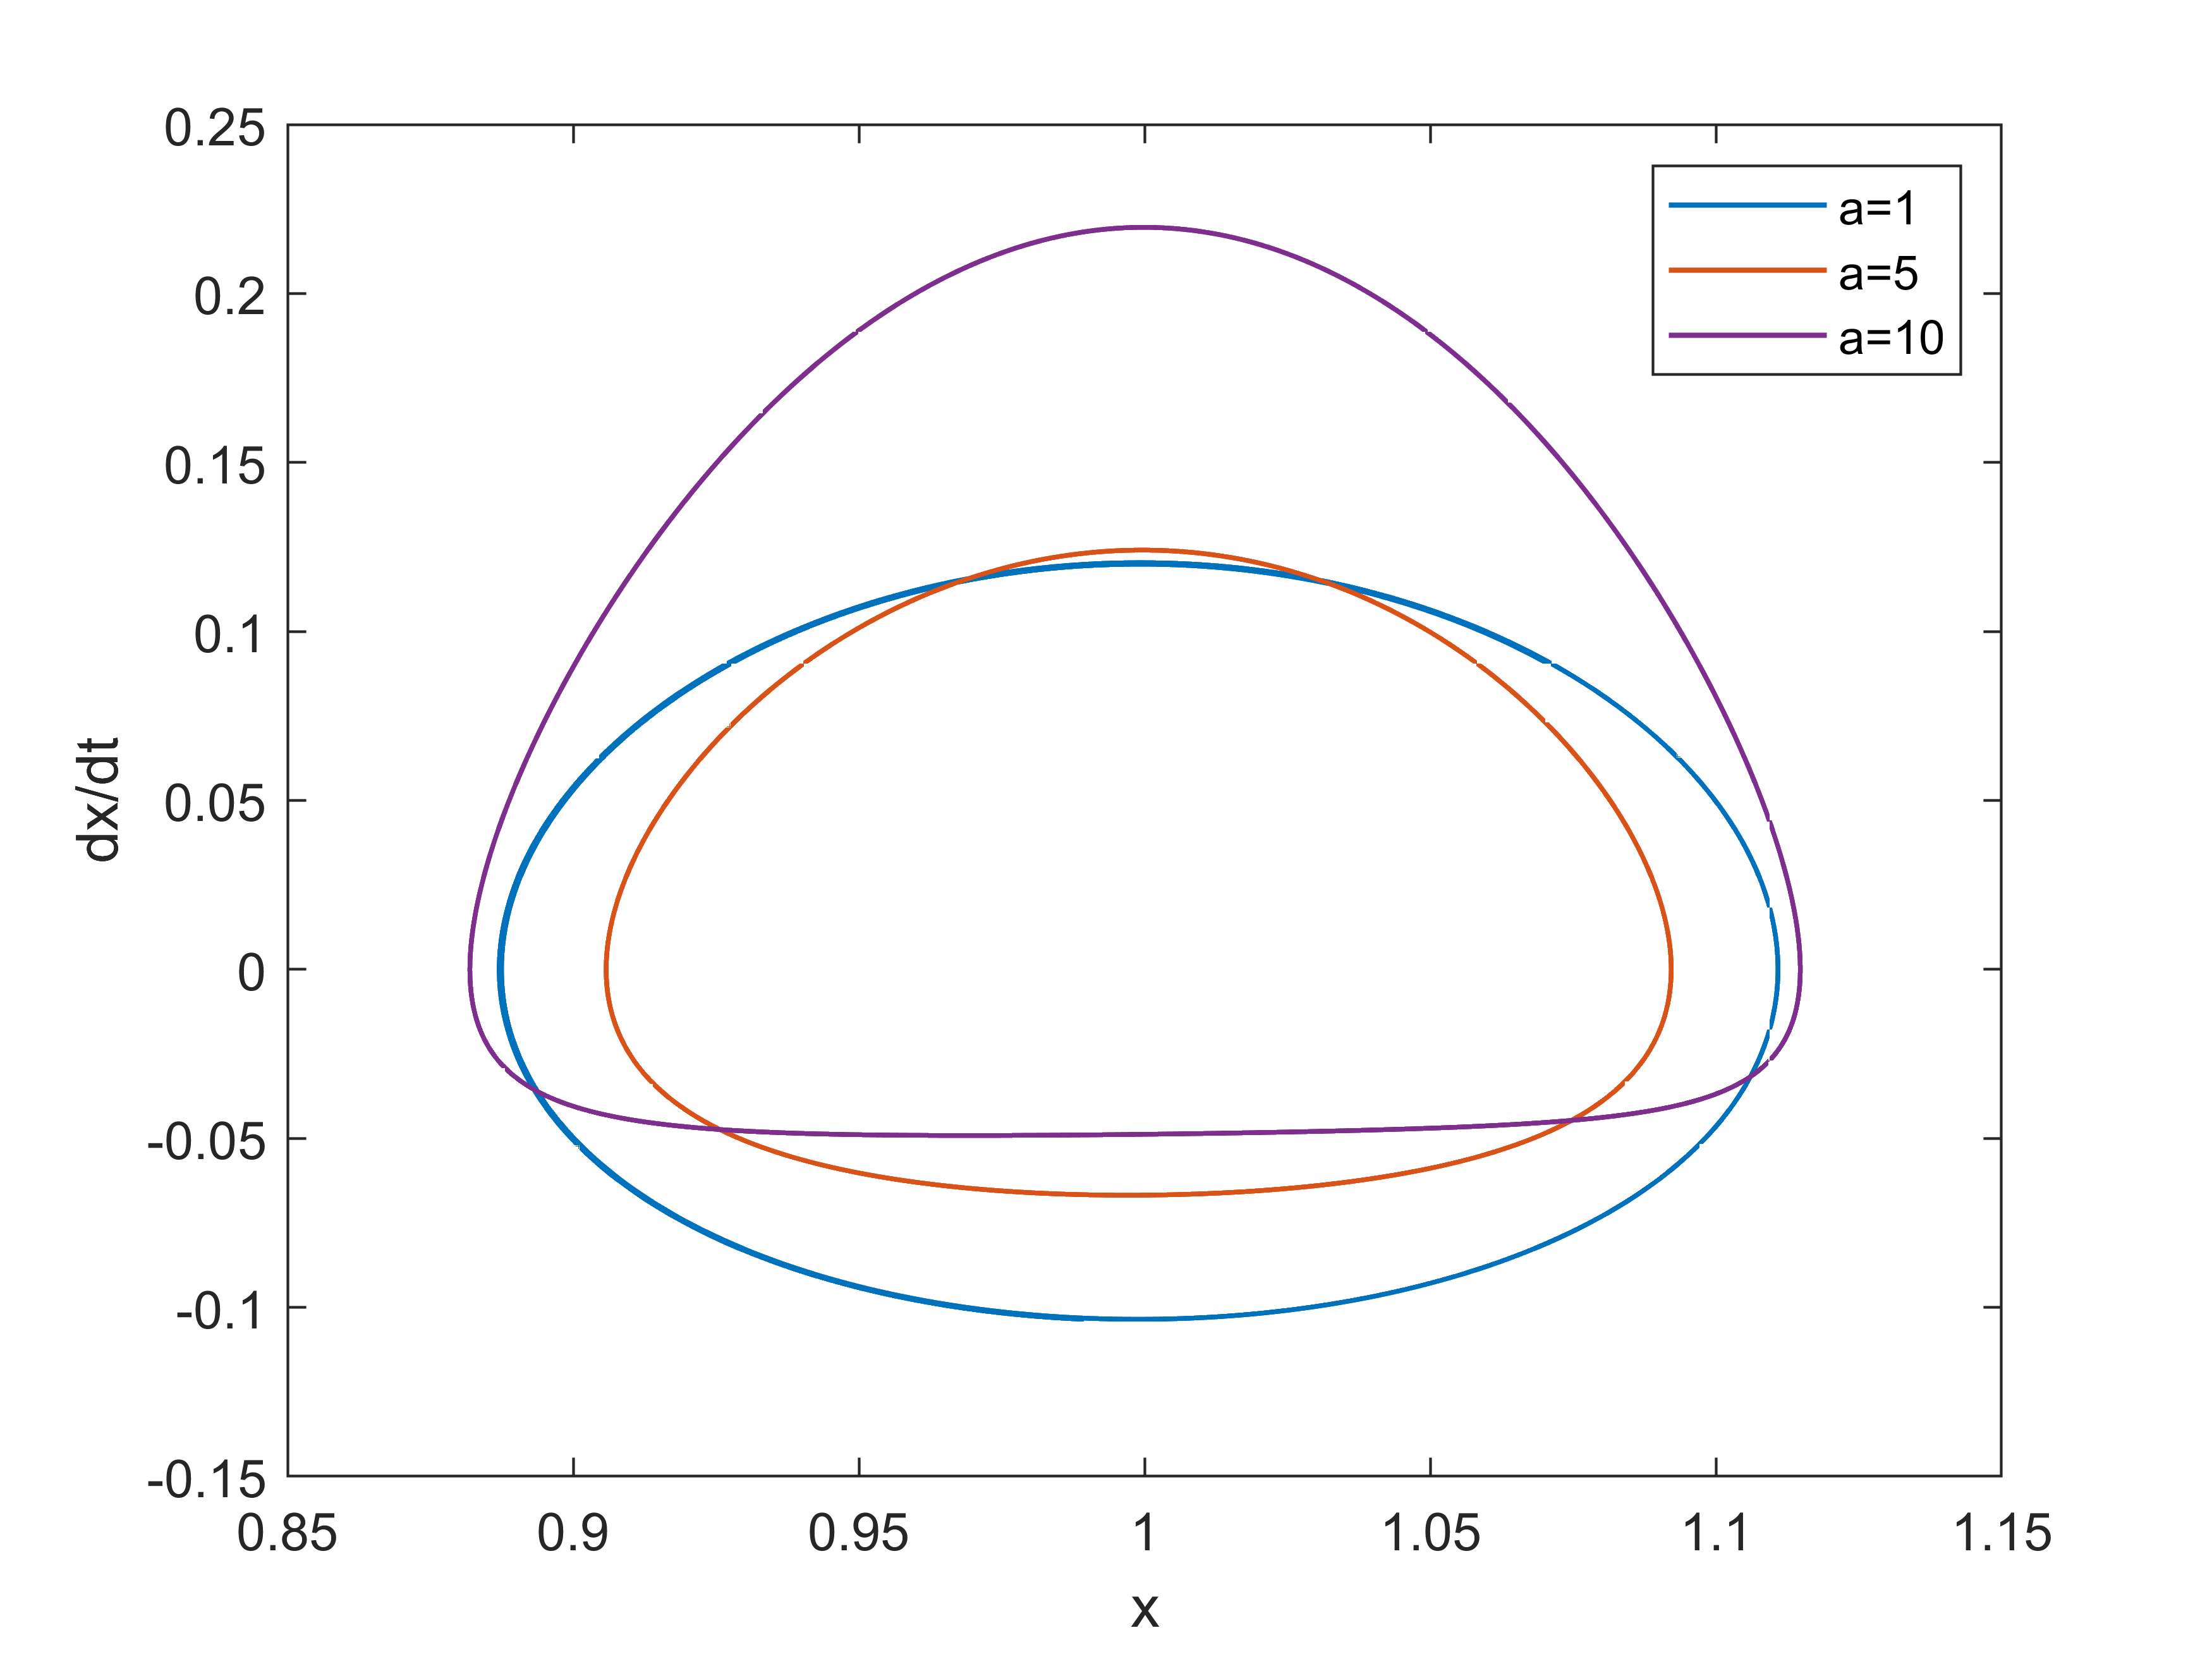
\includegraphics[width=0.45\textwidth]{Files/q8.png}
\caption{Graph of periodic orbits for $b=-0.001,a=1,5,10$ on $x(t)$ against $\dot{x}(t)$}
\end{figure}

\subsection*{Question 9}
\begin{figure}[H]
\centering
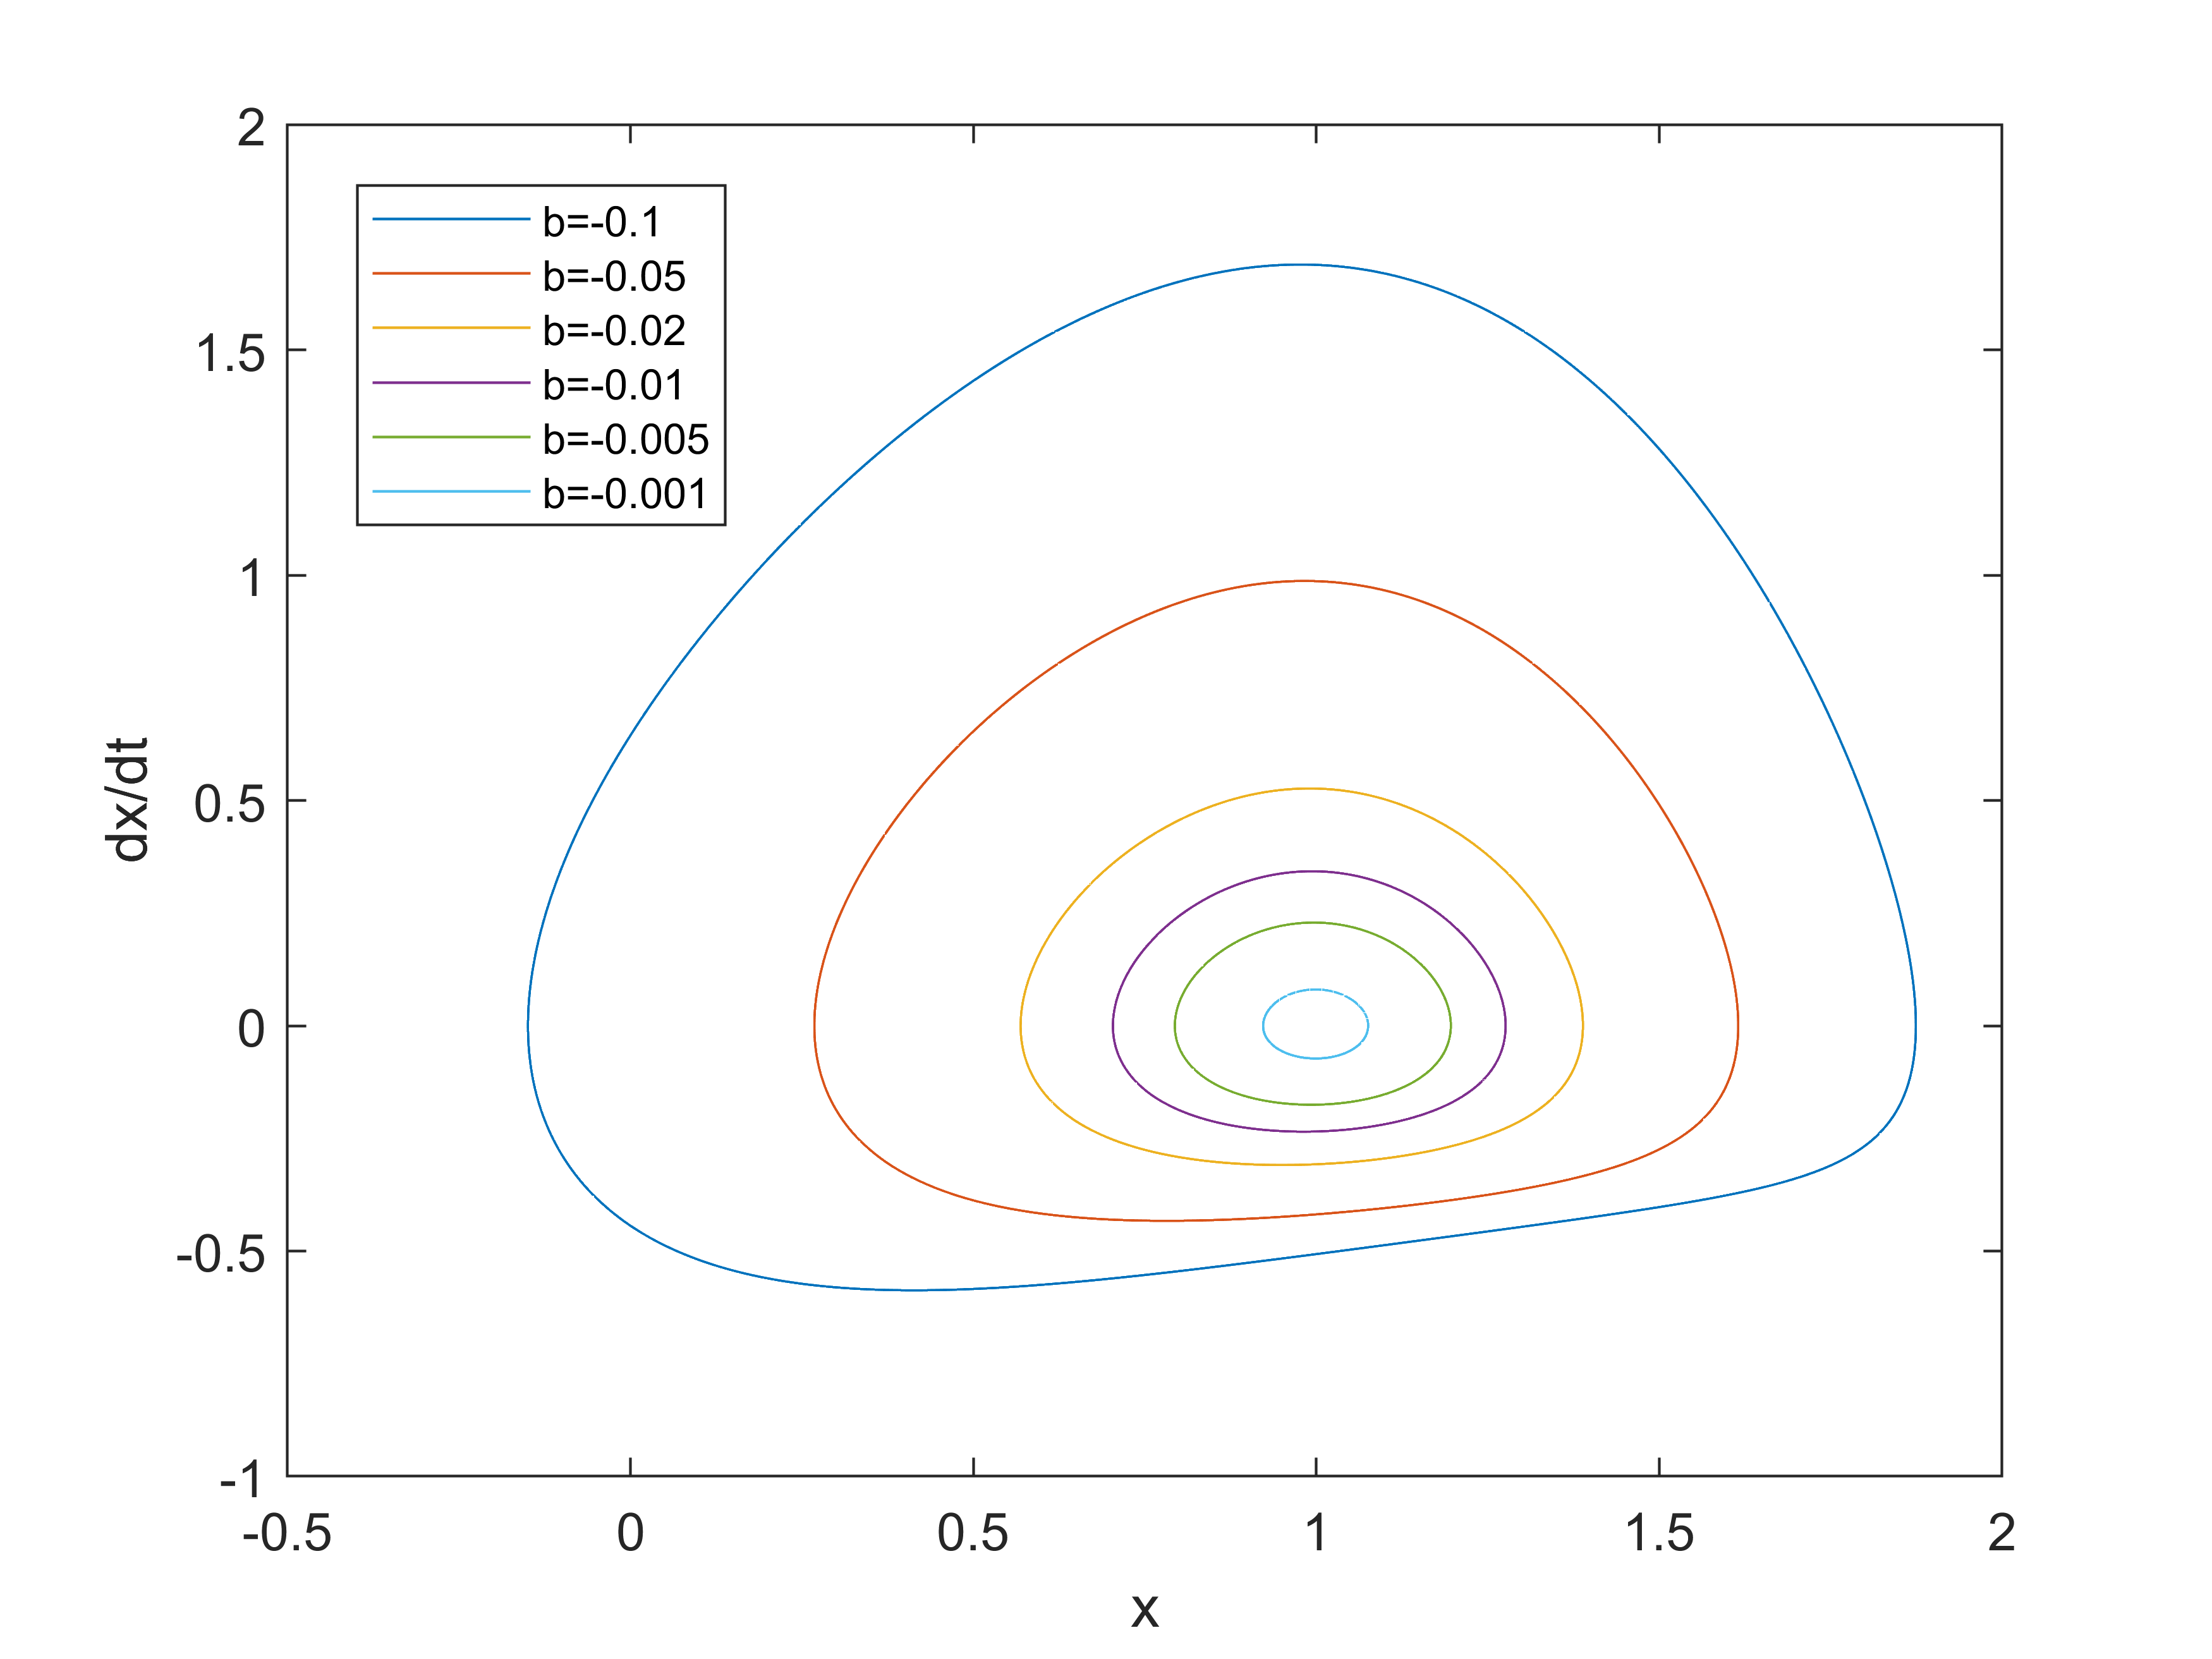
\includegraphics[width=0.45\textwidth]{Files/q9,a=1.png}
\caption{Graph of periodic orbits for $a=1, b\in[-0.1,0)$ on $x(t)$ against $\dot{x}(t)$}
\end{figure}
When $a=1$, the shape of the periodic orbit for $b\in[-0.1,0)$ are mostly similar. The change is only observed in their size, which decreases as $|b|$ decreases, and the decrease is roughly proportional to the size of $|b|$.\\
However, when $a=5,10$, as values of $b$ decreases, the shape of the periodic orbit changes massively.\\
\begin{figure}[H]
\centering
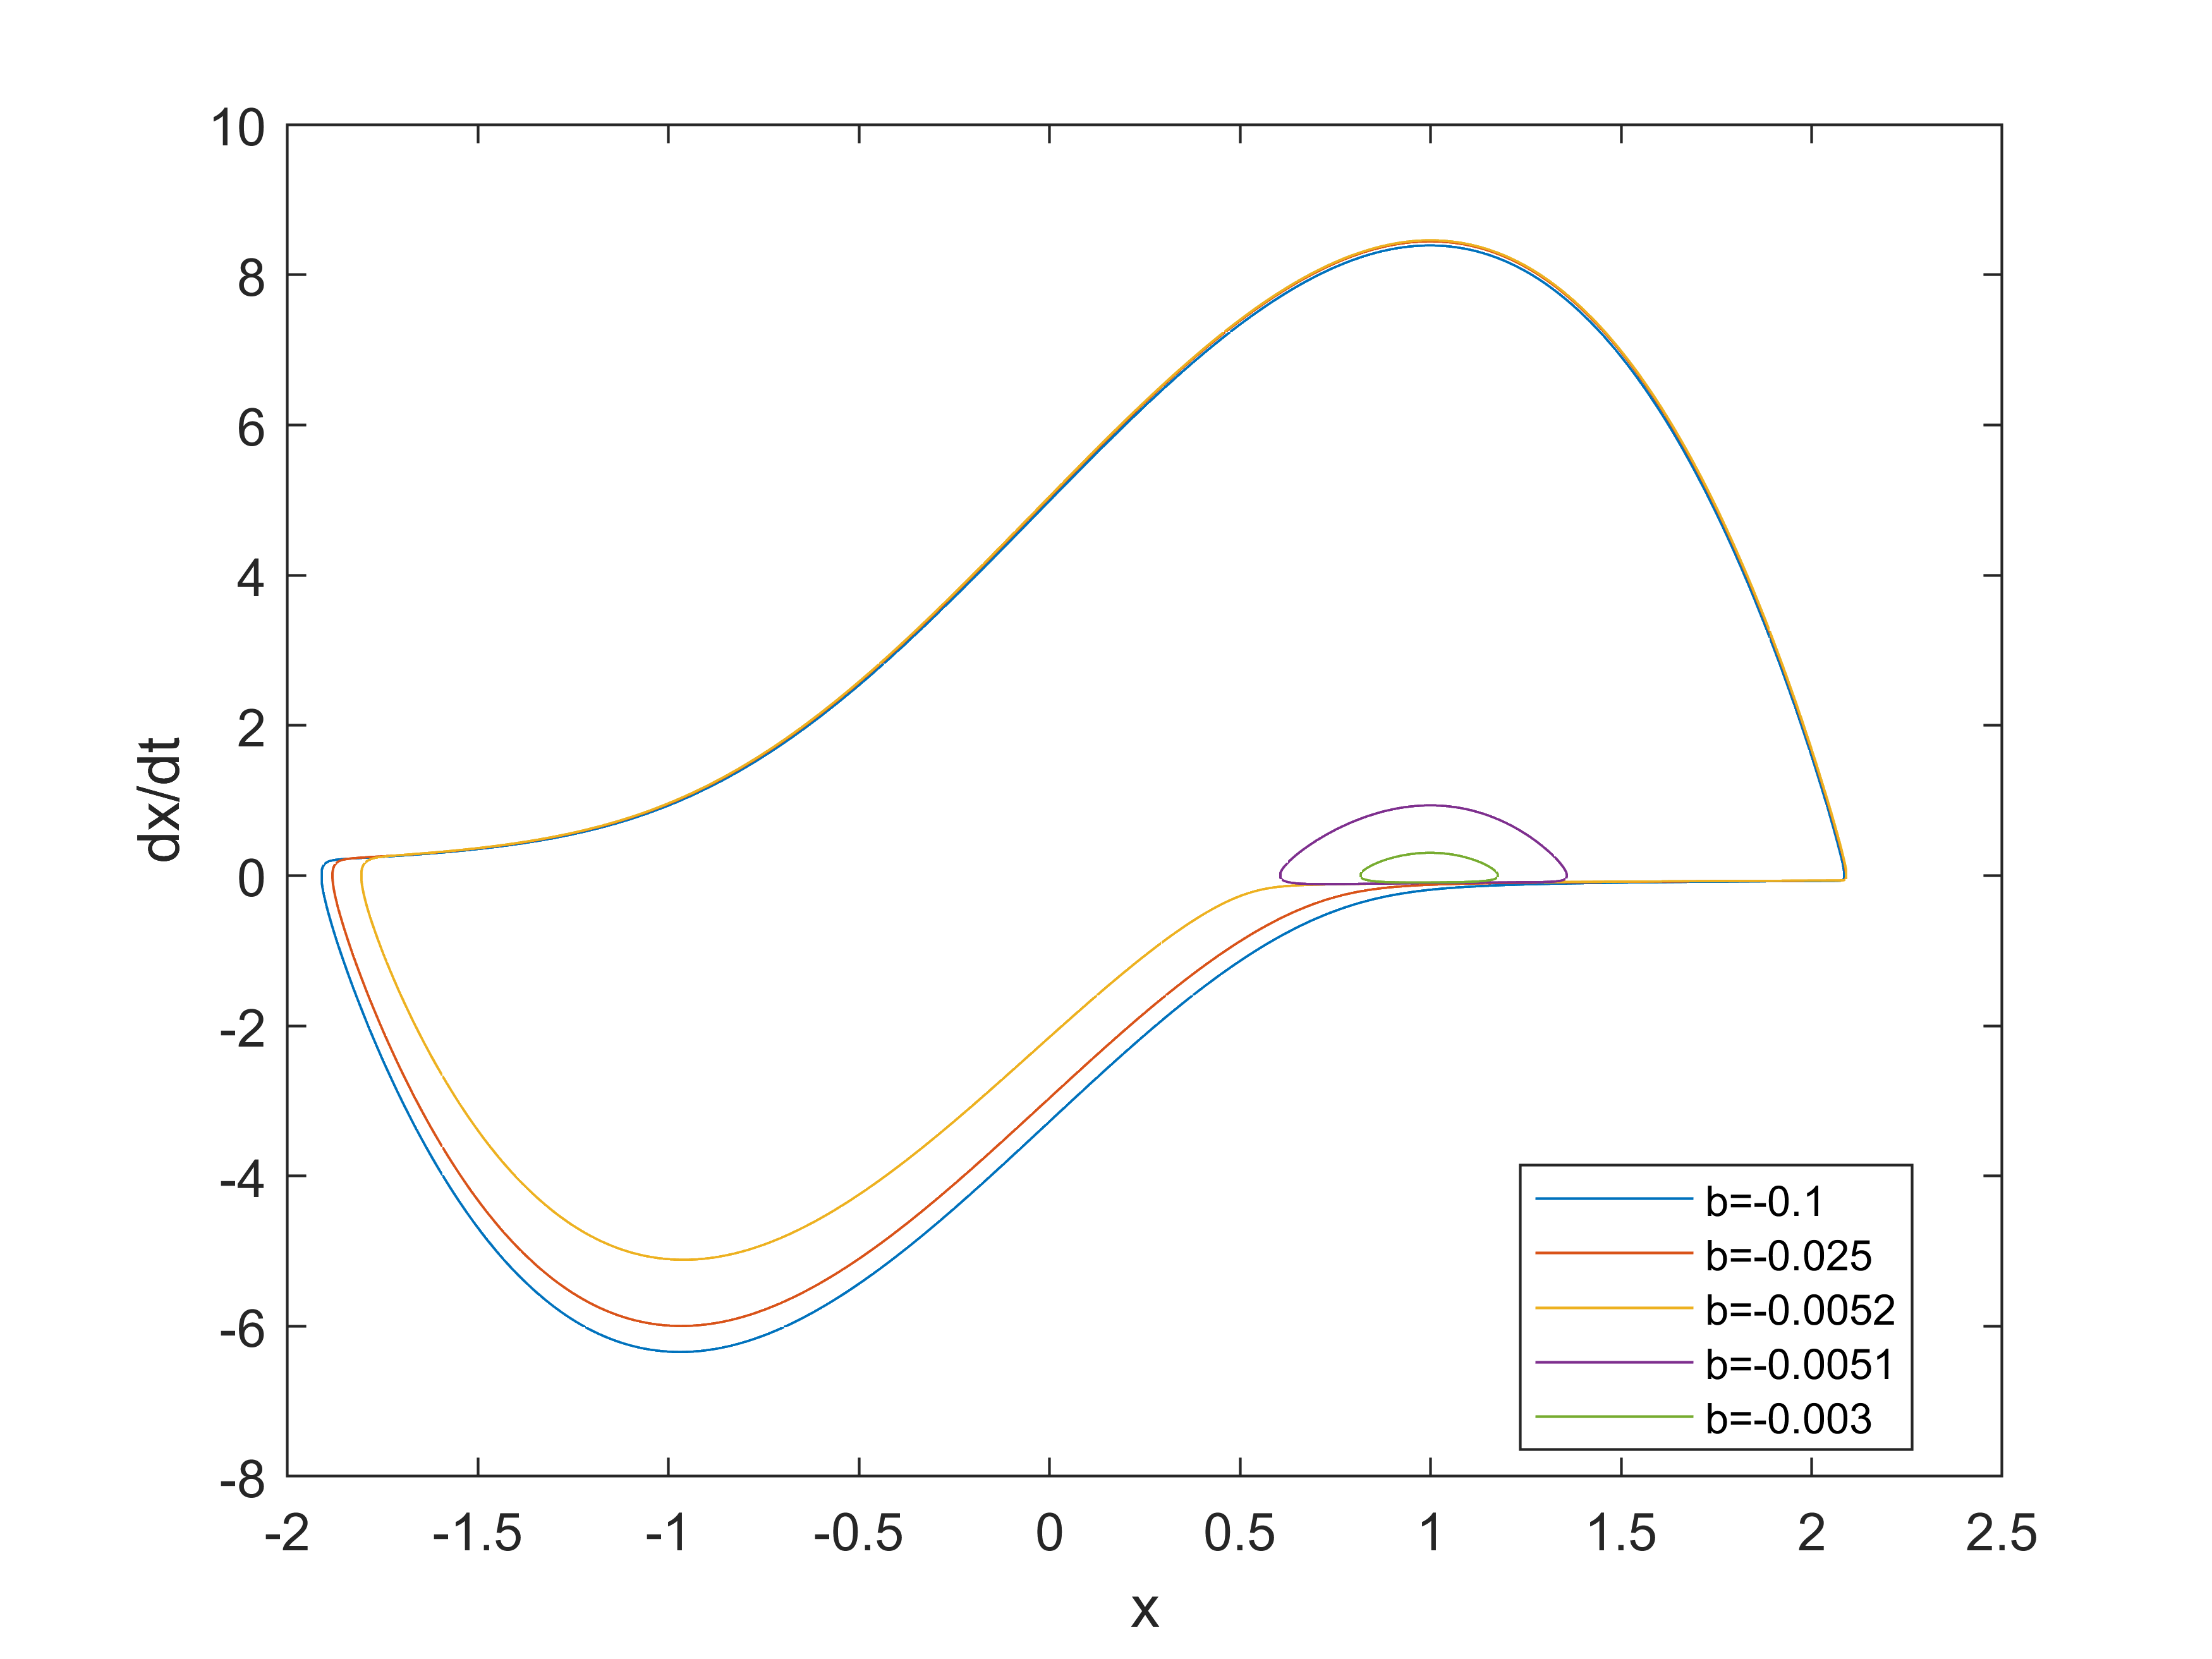
\includegraphics[width=0.55\textwidth]{Files/q9,a=5.png}
\caption{Graph of periodic orbits for $a=5, b\in[-0.1,0)$ on $x(t)$ against $\dot{x}(t)$}
\end{figure}
\noindent When $a=5$ and $b\leq-0.0052$, we see the periodic orbit has a shape which looks like an unforced van der Pol oscillator with fixed point at $(1+b,0)$ instead of $(0,0)$. And varying the value of $b$ from $-0.1$ to $-0.0052$ has no significant impact on the shape or size of the periodic orbit, since it's dominated by the size of $a$. We can only see a very small increase in $\frac{dx}{dt}$ near $x=-1$ as $|b|$ decreases.\\
However, when $b\geq -0.0051$, the periodic orbit changes to a completely different shape, which is roughly like an ellipse and similar to what we observed in question 8, this is probably because $1+b$ starts to dominate over $a(x^2-1)y$ near the fixed point.

\begin{figure}[H]
\centering
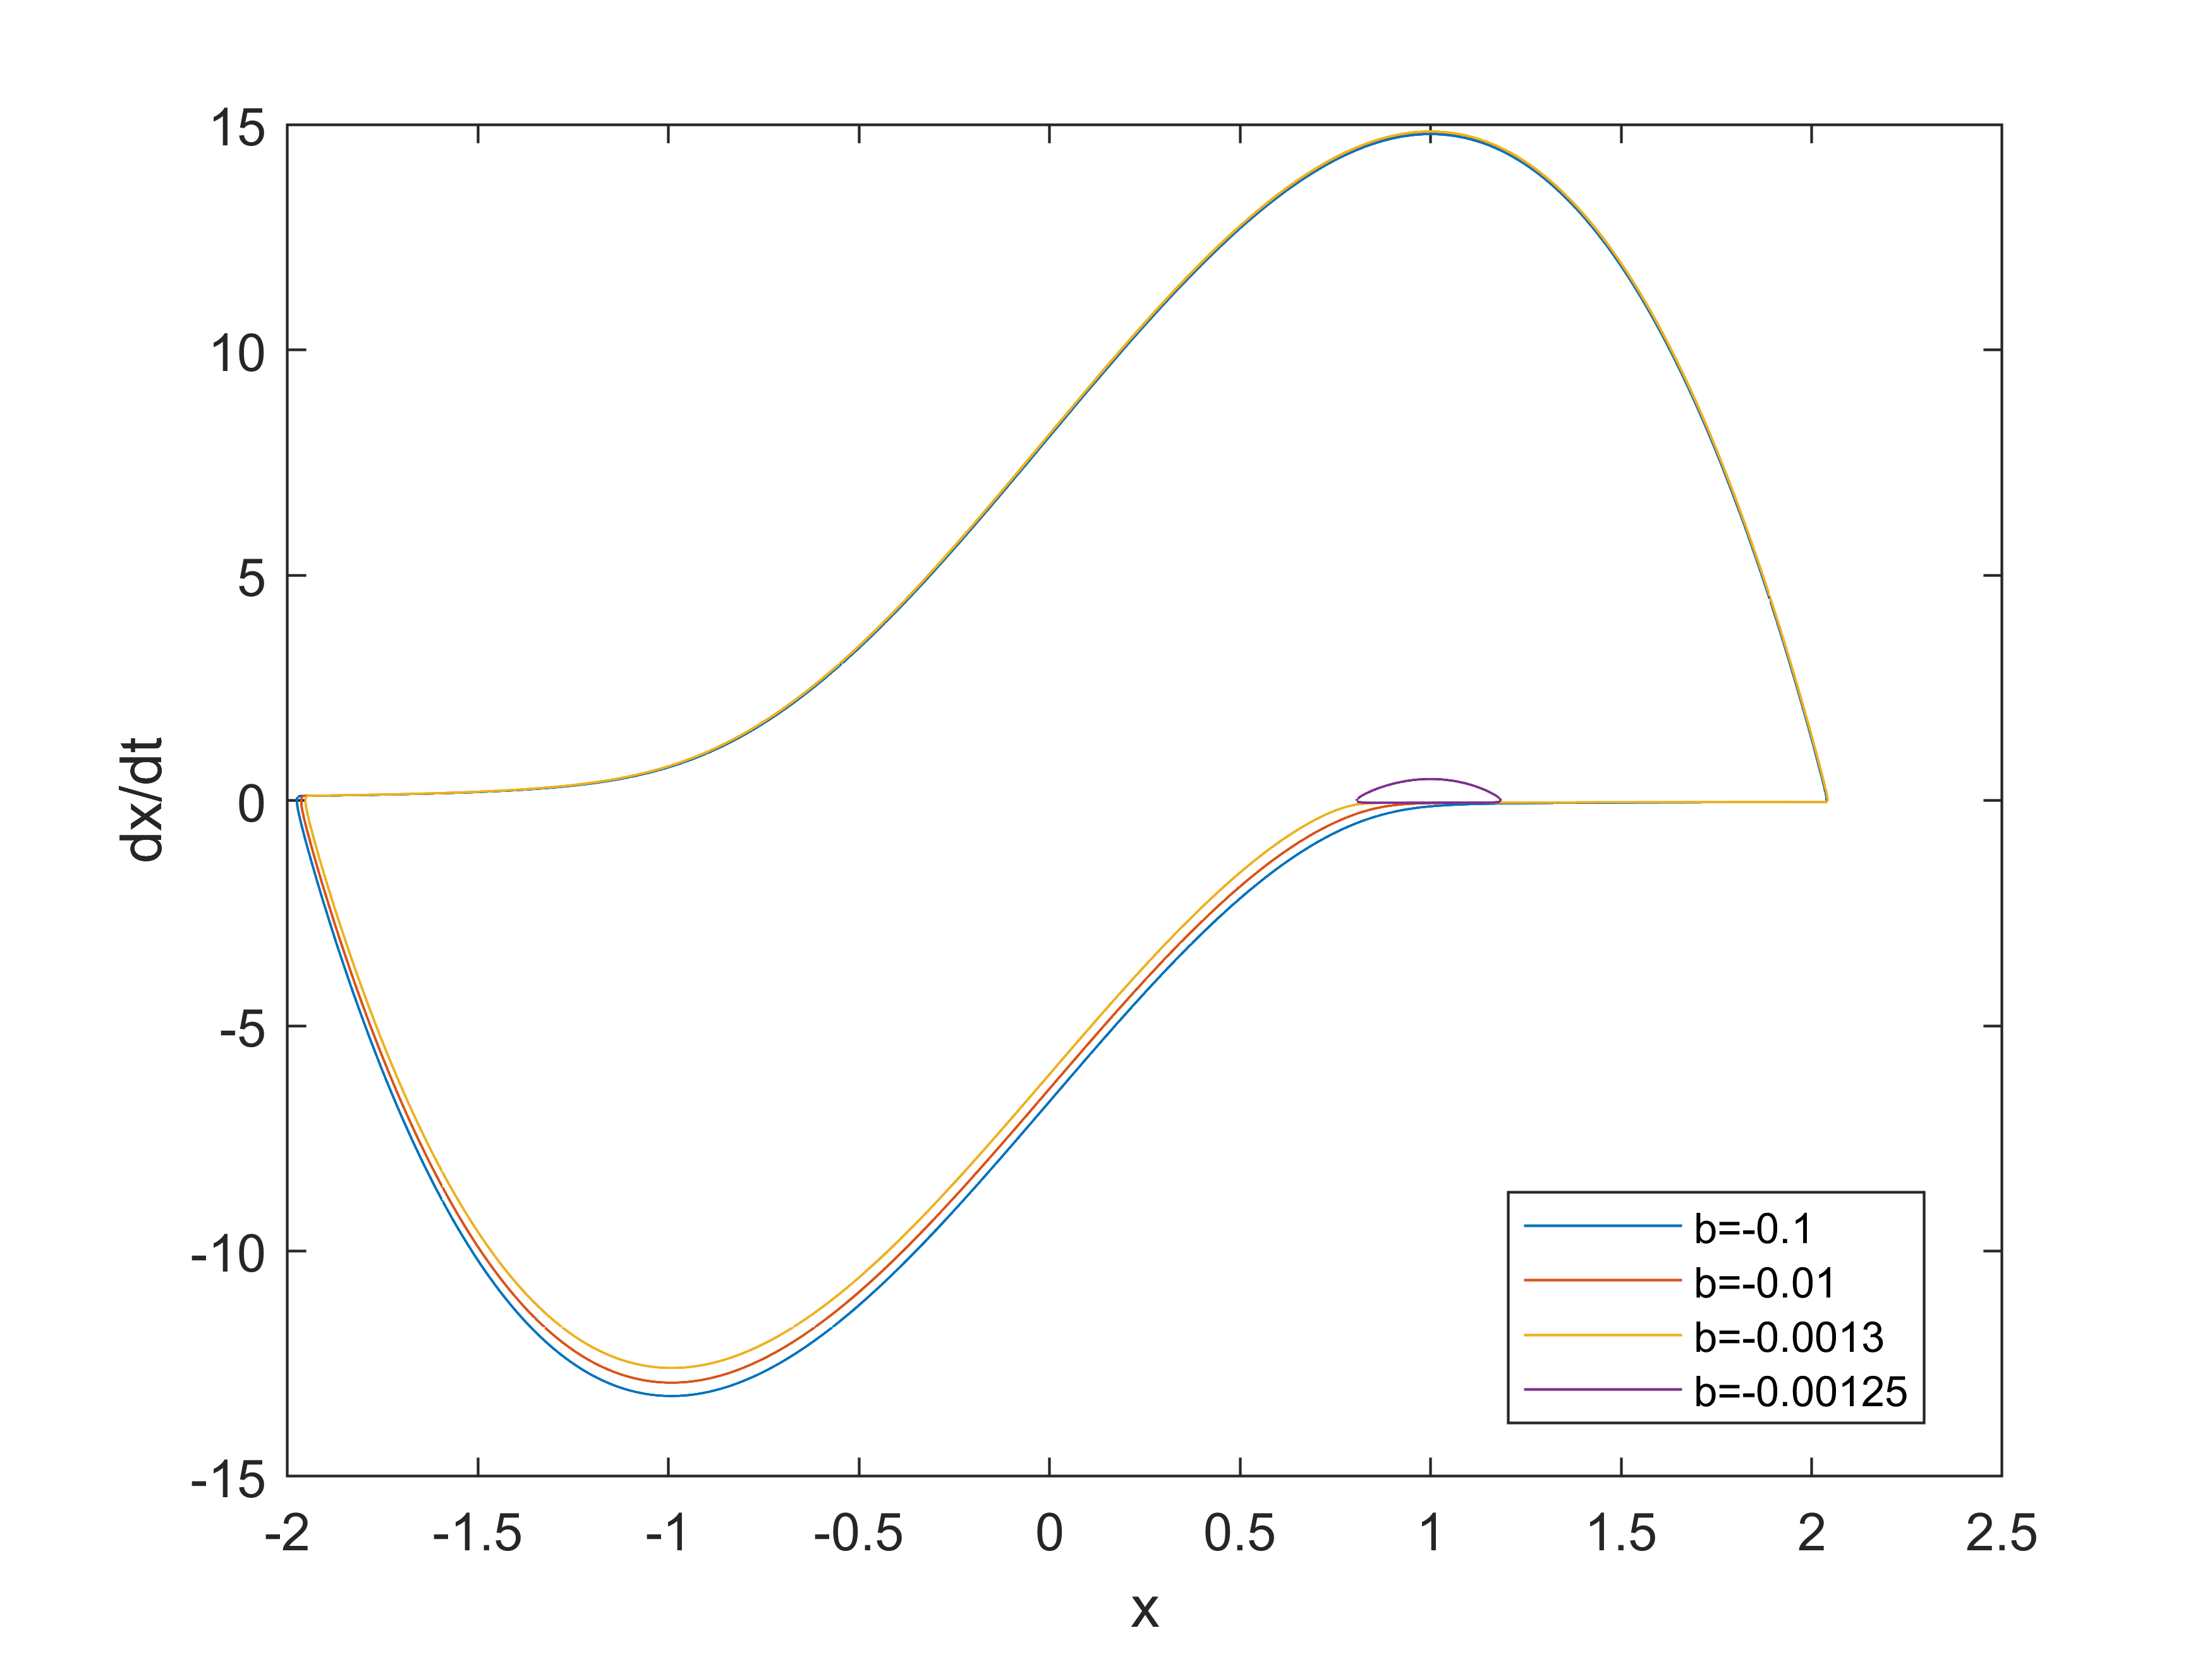
\includegraphics[width=0.55\textwidth]{Files/q9,a=10.png}
\caption{Graph of periodic orbits for $a=10, b\in[-0.1,0)$ on $x(t)$ against $\dot{x}(t)$}
\end{figure}
\noindent When $a=10$ and $b\leq-0.0013$, we see that again the periodic orbit has a shape which looks like an unforced van der Pol oscillator with fixed point at $(1+b,0)$ instead of $(0,0)$. And varying the value of $b$ from $-0.1$ to $-0.0013$ has no significant impact on the shape or size of the periodic orbit, since it's dominated by the size of $a$. We can only see a very small increase in $\frac{dx}{dt}$ near $x=-1$ as $|b|$ decreases.\\
However, when $b\geq -0.0013$, the periodic orbit changes to a completely different shape, which is roughly like an ellipse and similar to what we observed in question 8, this is probably because $1+b$ starts to dominate over $a(x^2-1)y$ near the fixed point.\\
This is very similar to what happened when $a=5$, the only difference is the value of $b$ which the behaviour happens. It's near $b=-0.0052$ when $a=5$ and near $b=-0.0013$ when $a=10$. We hence note that $b|_{a=5}\approx 4 \cdot b|_{a=10}$, which is $2^2$. So a reasonable guess is that for large values of $a$, whenever $a$ is doubled, $1/b$ is quadrupled, for $b$ where the drastic change of periodic orbit occurs.\\
This can be explained by expanding $\dot{y}$ near the fixed point $(1+b,0)$, i.e. by letting $x=1+b+\epsilon(t),y=\mu(t)$. We get $\dot{\mu}=-\epsilon-a(2b+b^2)\mu$ accurate to linear terms.\\
We note that the dominant coefficient is $-ab^2$, hence the value of $1/b$ where the significant change occurs is quadrupled when $a$ is doubled.\\\\ 


\noindent The program used to plot these graphs can be found in the programs section under the title \emph{'viii) q9.m'}. The program is very similar to the one we used in question 8. The only difference is now we are varying $b$ rather than $a$. The initial conditions I used for $b$ in each diagram can be found in the legend. I've also decreased $h$ from 0.001 to 0.0001 for better accuracy. \\
Another point to note is that as $a$ increases, we need to adjust accordingly which points to plot.\\
For $a=1$, plot when $t=[4990,5000]$; for $a=5$, plot when $t=[4900,5000]$; and for $a=10$, plot when $t=[4800,5000]$. This is because the time period is proportional to the value of $a$ especially for small values of $b$.

\subsection*{Question 10}
We write the equation in Li\'{e}nard coordinates as 
\[\left
\{\begin{array}{lr}
\dot{x}= y-a(\frac{x^3}{3}-x)\\
\dot{y}= -x+1+b
\end{array}
\right.
\]
The program used to plot the graph below can be found in the programs section under the title \emph{'ix) q10.m'}.\\
We'll use the case where $a=10$ as an example for the shape of the periodic orbit when $a$ is large.
\begin{figure}[H]
\centering
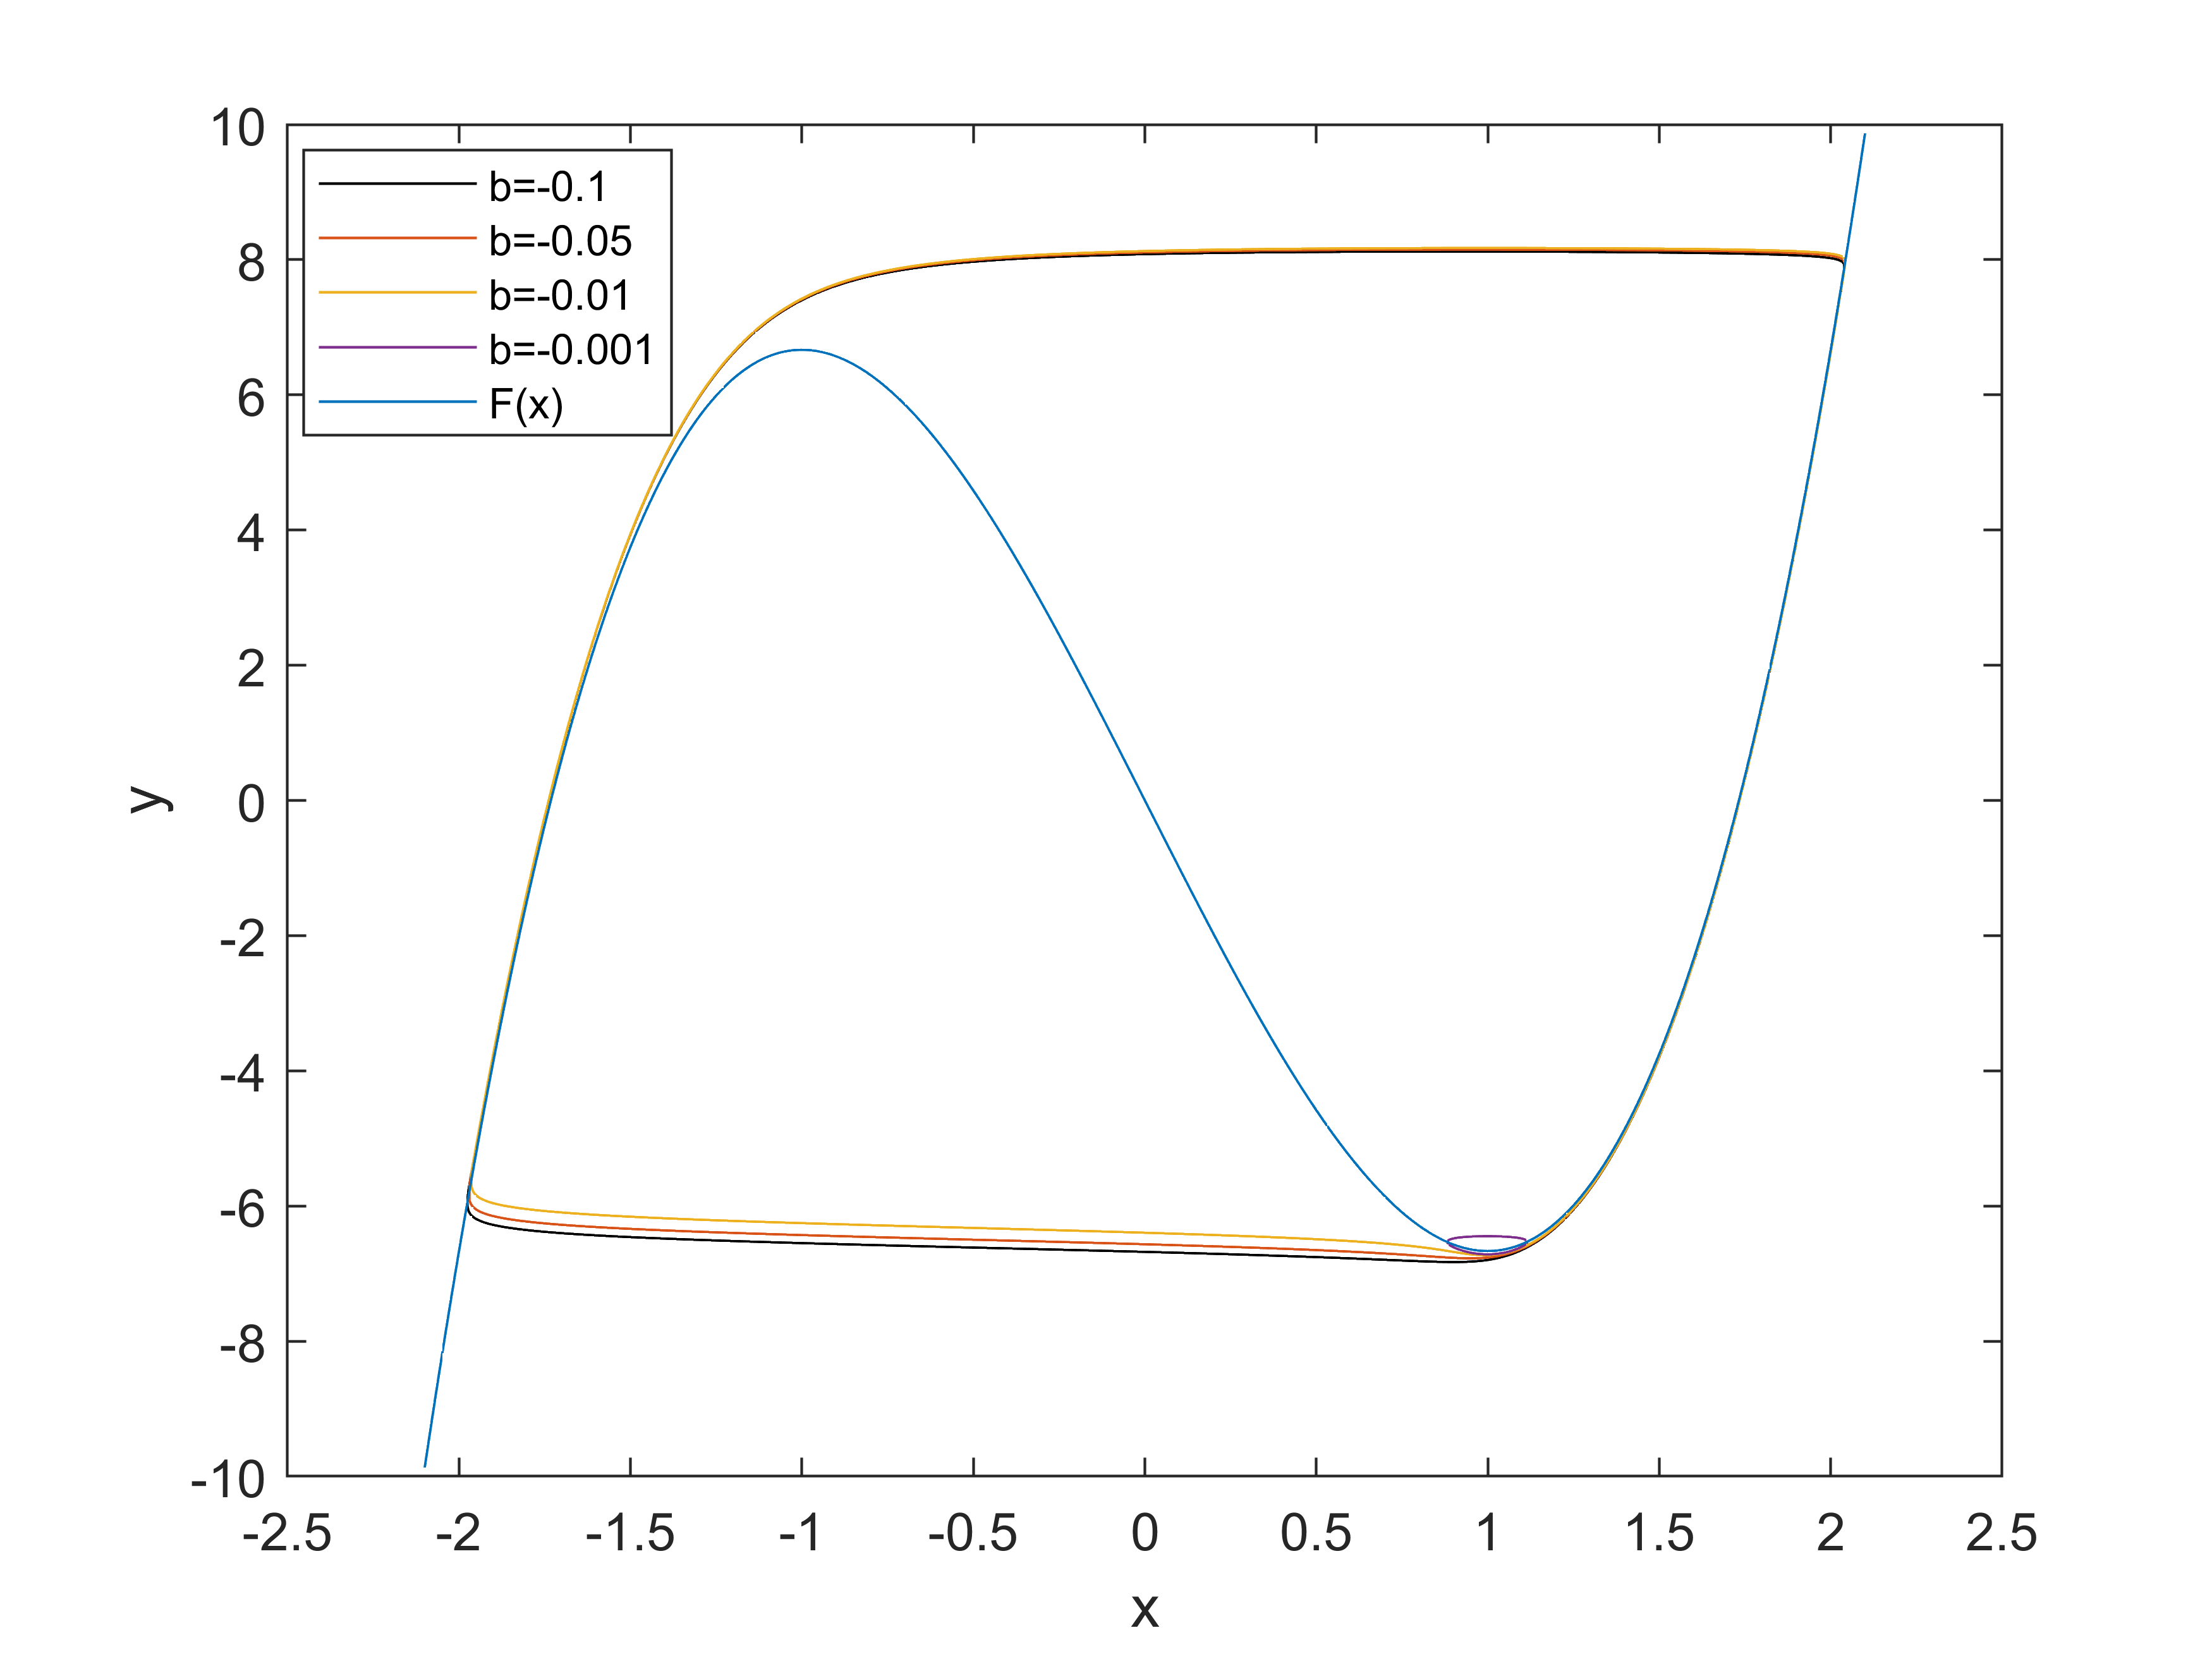
\includegraphics[width=0.6\textwidth]{Files/q10,a=10.png}
\caption{Graph of periodic orbits for $a=10, b\in[-0.1,0)$ in the x-y plane}
\end{figure}
\noindent For large values of $a$, as $\dot{x}=y-a(\frac{x^3}{3}-x)$, $\dot{x}$ dominates unless near $y=F(x)$, where $F(x)=a(\frac{x^3}{3}-x)$.\\
Looking at $F(x)$, we note that it has a maximum at $(-1,\frac{2}{3}a)$ and a minimum at $(1,\frac{-2}{3}a)$. We can show this by differentiating $F(x)$ and equate it to 0, which gives us $a(x^2-1)=0$, hence $x=\pm1$. Plugging these into $F(x)$ gives $a(\frac{(\pm1)^3}{3}-\pm1)=\frac{\mp2}{3}a$.\\
We plot $F(x)$ on the graph along with the periodic orbits. We note that for $b=-0.1,-0.05,-0.01$, the periodic orbit moves closely to $F(x)$ from near $(-2,\frac{-2}{3}a)$ to the maximum $(-1, \frac{-2}{3}a)$ as this is where $\dot{y}$ dominates over $\dot{x}$. It then overshoots $F(x)$ and moves almost horizontally rightward to near $(2,\frac{2}{3}a+1)$. It then again follows closely $F(x)$ from around $(2,\frac{2}{3}a+1)$ to $(1,\frac{-2}{3}a)$, where it overshoots slightly and then moves leftward almost horizontally to $(-2,\frac{-2}{3}a)$, where it intersects $F(x)$ again.\\
The reason for the shape of the periodic orbit is precisely that $\dot{x}$ is dominated near $y=F(x)$, so once the orbit is near $F(x)$, it will follow closely to it. So starting from $(-2,\frac{-2}{3}a)$, the orbit follows $F(x)$ and only after we've passed the maximum of $F(x)$, that $\dot{x}$ is now large and positive for the periodic orbit whereas $\dot{y}=-x+1+b$ is small in comparison. We know this since $\dot{x}$ is $\mathcal{O}(a)$ whereas $\dot{y}$ is $\mathcal{O}(1)$. Similar things happen again once the periodic orbit is near $(2,\frac{2}{3}a+1)$. Now, $\dot{y}$ dominates again so the orbit follows $F(x)$ closely until the minimum near $(1,\frac{-2}{3}a)$. Then, $\dot{x}$ would again dominate and the orbit goes almost horizontally leftwards.\\
\begin{figure}[H]
\centering
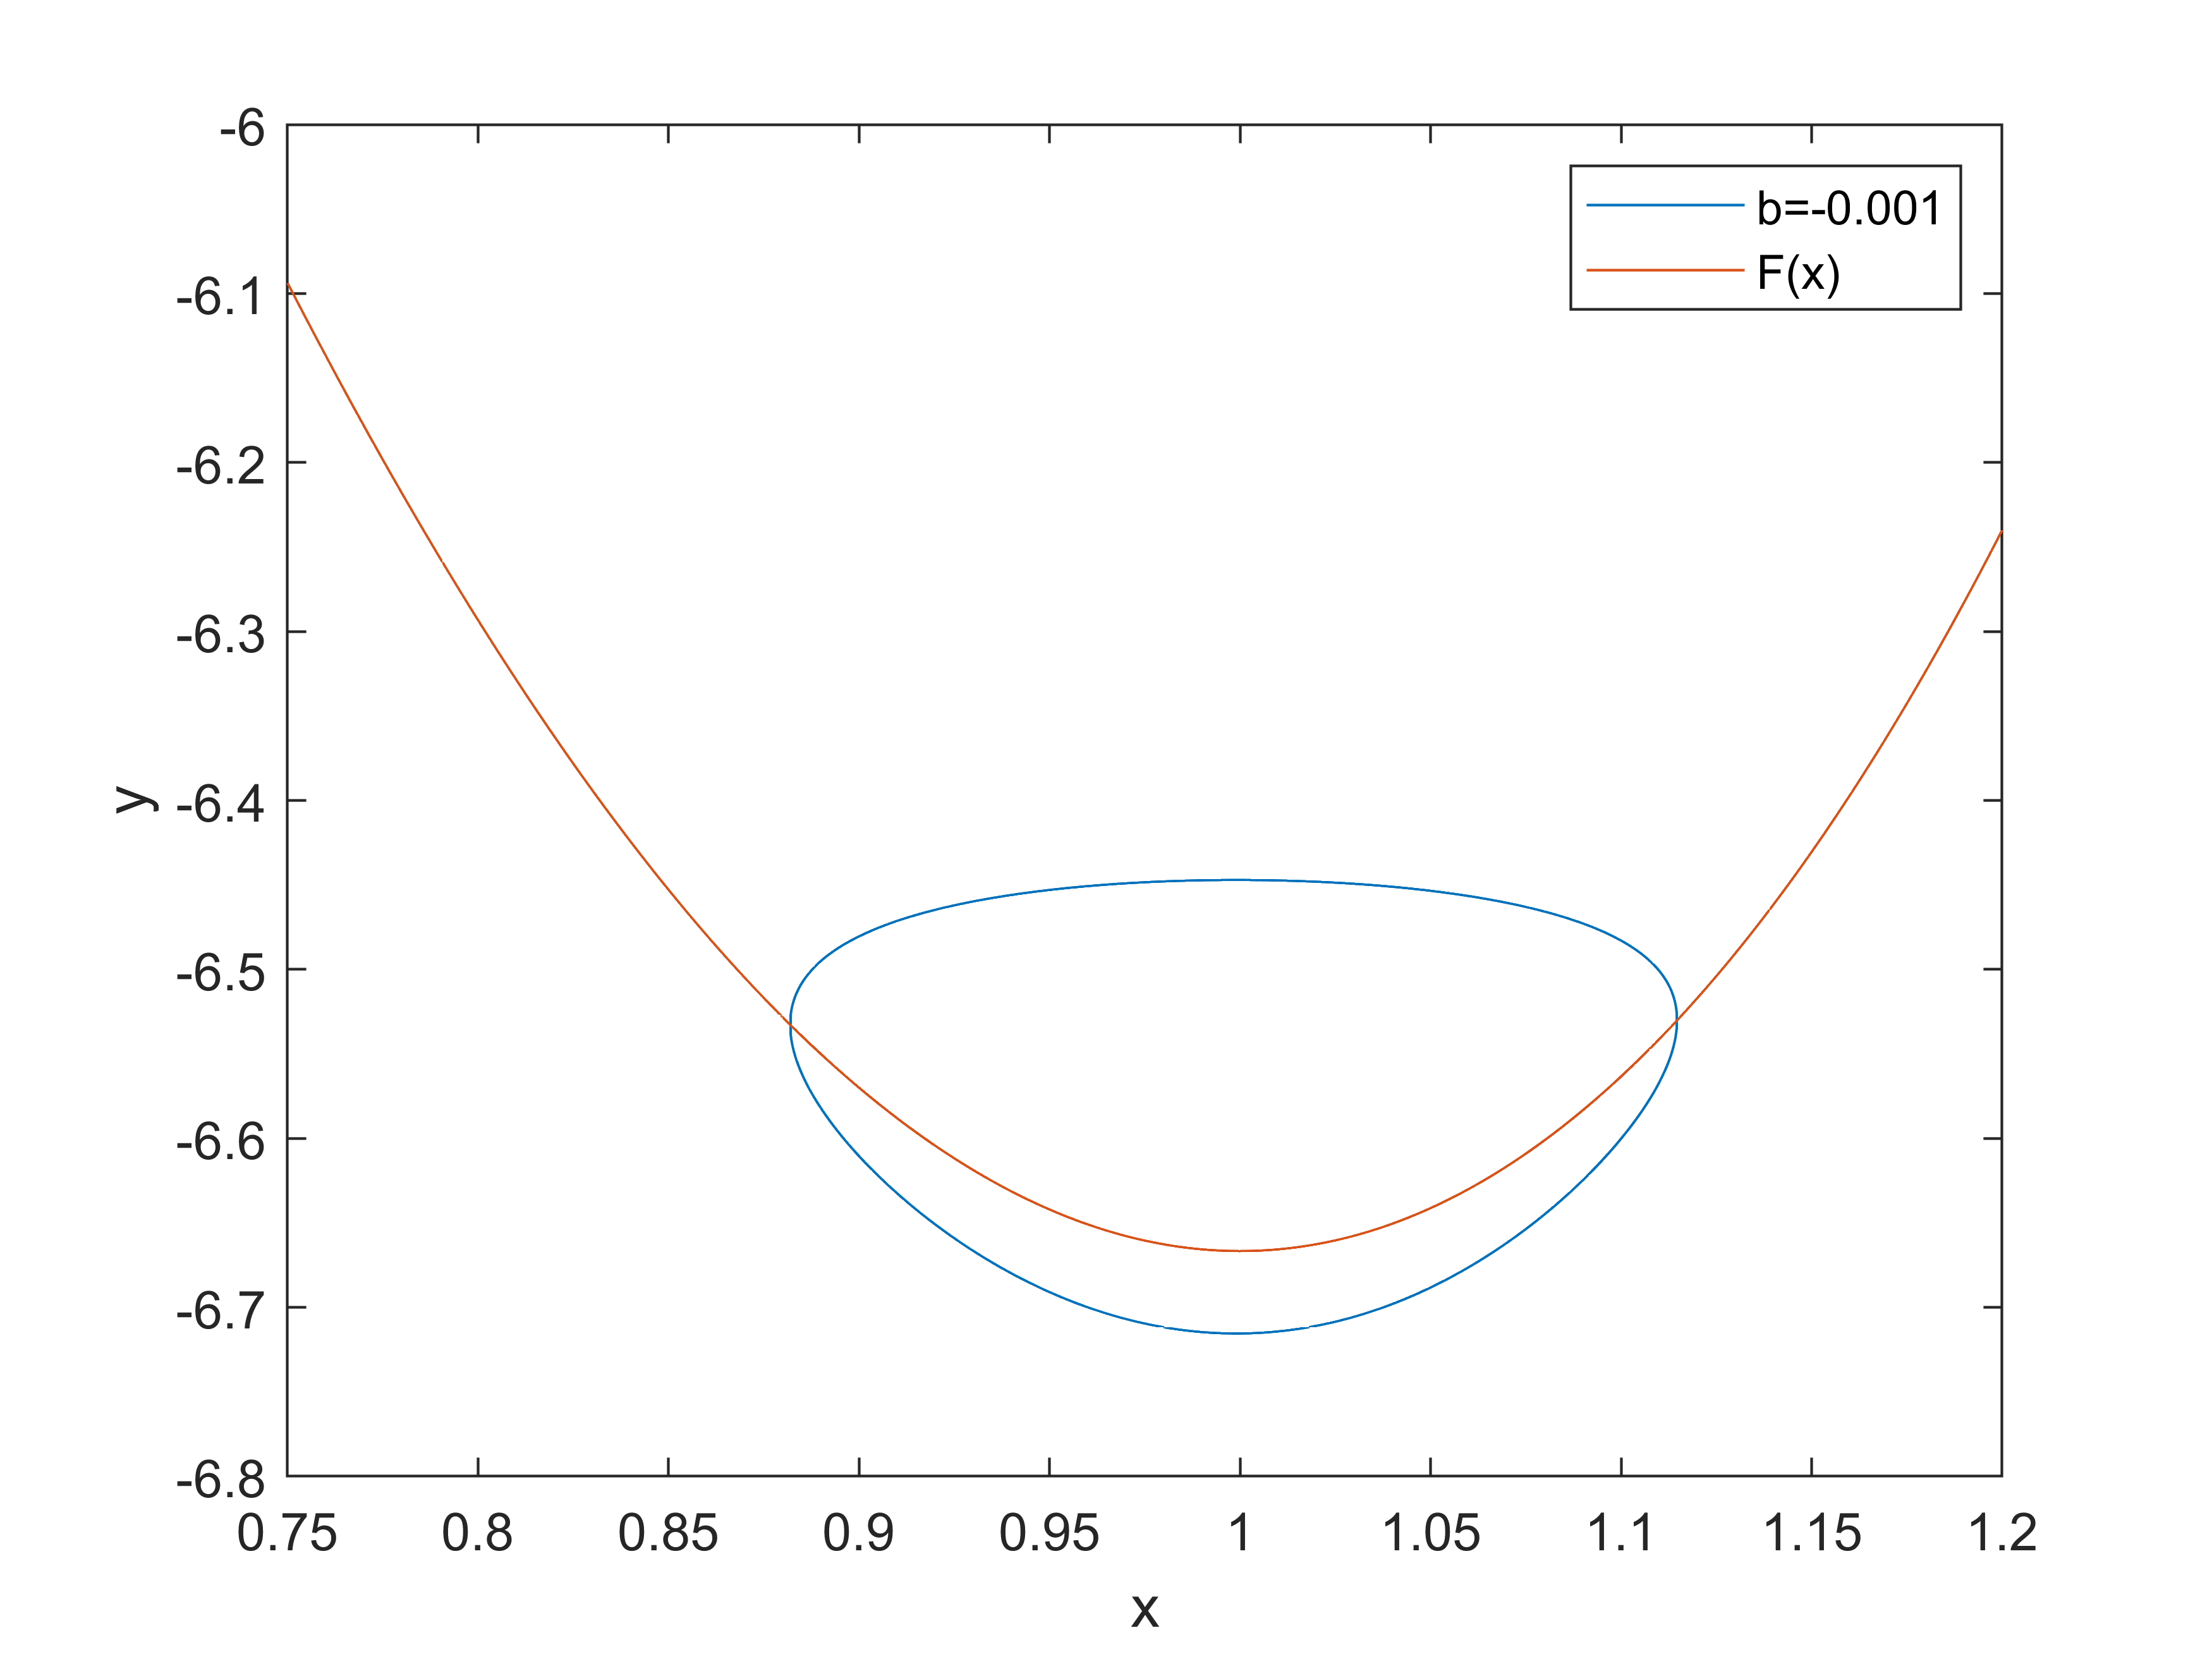
\includegraphics[width=0.45\textwidth]{Files/q10,a=10,2.png}
\caption{Graph of periodic orbit for $a=10$ and $b$ small in the x-y plane}
\end{figure}
\noindent And when $b$ is sufficiently small, after the periodic orbit crosses $F(x)$ on the right, because $\dot{y}=-x+1+b$, it is large enough such that the orbit follows $F(x)$ around the minimum and crosses $F(x)$ immediately to the left of the minimum, so it has a much smaller periodic orbit than when $|b|$ is larger.\\\\
The numerical difficulty in calculating such orbits arise because of the difference in time taken to travel from $A=(-2,\frac{-2}{3}a)$ to $B=(-1,\frac{2}{3}a)$ and $B=(-1,\frac{2}{3}a)$ to $C=(2,\frac{2}{3}a+1)$. By symmetry, the time taken from $C$ to $D=(1,\frac{-2}{3}a)$ is similar to from $A$ to $B$; similar time from $D$ to $A$ as from $B$ to $C$.\\
We note from $A$ to $B$, $\dot{y}=\mathcal{O}(1)$ and the difference in $y\approx\frac{4}{3}a$, which is $\mathcal{O}(a)$. Hence, the time taken to travel from $A$ to $B$ is $\mathcal{O}(a)$.\\
However, from $B$ to $C$, $\dot{x}=\mathcal{O}(a)$ and the difference in $x$ is $\mathcal{O}(1)$. Hence, the time taken to travel from $B$ to $C$ is $\mathcal{O}(a^{-1})$.\\
Therefore, to plot the orbit accurately, we must use a time step $h$ that's much smaller than $\mathcal{O}(a^{-1})$, so that we can plot the orbit from $B$ to $C$ and $D$ to $A$ accurately. And we must plot it over a range of time that's much larger than $\mathcal{O}(a)$ to plot the orbit from $A$ to $B$ and $C$ to $D$. Whilst this is not a problem when $a=10$, we will soon be in trouble for larger $a$. And this requirement for a smaller $h$ and larger $t$ will significantly increase the amount of time for the computer to numerically integrate the equations, since we now have a much larger number of total iterations to compute, and the time complexity of the algorithm is proportional to the number of iterations taken.


\newpage
\section*{Programs}
\subsection*{i) q1.m}
\lstdefinestyle{myCustomMatlabStyle}{
  language=Matlab,
  stepnumber=1,
  numbersep=10pt,
  tabsize=4,
  showspaces=false,
  showstringspaces=false
}
\lstset{basicstyle=\footnotesize,style=myCustomMatlabStyle}
\begin{lstlisting}
format long
initial_x = [-1.3,-1,0.1,0.9,1.6];   % choice of initial condition for x(0)
initial_y = [-1.3,-0.01,0.1,0.3,1];     % choice of initial condition for dx/dt(0)
b = 0;      % coefficients in equation
a = -0.12;
n = 100000;      % number of total steps
endpoint = 70;   % end point of t 
t = linspace(0,endpoint,n);  % starting and ending point of t
h = t(2)-t(1);    % step size
for i = 1:5
    x = zeros(n,1);
    y = zeros(n,1);
    f = @(t,x,y) y;     % formula for dx/dt
    g = @(t,x,y) -a*y+x-x^3+b*cos(t);     %formula for dx^2/dt^2
    x(1) = initial_x(i);     % initial value of x
    y(1) = initial_y(i);     % initial value of y=dx/dt
    for j=1:n-1
        k1 = f(t(j),x(j),y(j));     % k is the RK4 for x
        l1 = g(t(j),x(j),y(j));     % l is the RK4 for y=dx/dt

        k2 = f(t(j)+0.5*h,x(j)+0.5*h*k1,y(j)+0.5*h*l1);
        l2 = g(t(j)+0.5*h,x(j)+0.5*h*k1,y(j)+0.5*h*l1);

        k3 = f(t(j)+0.5*h,x(j)+0.5*h*k2,y(j)+0.5*h*l2);
        l3 = g(t(j)+0.5*h,x(j)+0.5*h*k2,y(j)+0.5*h*l2);

        k4 = f(t(j)+h,x(j)+h*k3,y(j)+h*l3);
        l4 = g(t(j)+h,x(j)+h*k3,y(j)+h*l3);

        x(j+1) = x(j)+(1/6)*h*(k1+2*k2+2*k3+k4); %updating values of x
        y(j+1) = y(j)+(1/6)*h*(l1+2*l2+2*l3+l4);    %updating values of y
    end
    plot(x,y,'DisplayName', sprintf('(%g,%g)', initial_x(i), initial_y(i)))
    hold on
end
xlabel('x')
ylabel('dx/dt')
legend()

\end{lstlisting}
\newpage
\subsection*{ii) q3.m}
\lstdefinestyle{myCustomMatlabStyle}{
  language=Matlab,
  stepnumber=1,
  numbersep=10pt,
  tabsize=4,
  showspaces=false,
  showstringspaces=false
}
\lstset{basicstyle=\footnotesize,style=myCustomMatlabStyle}
\begin{lstlisting}
format long
initial_x = [-1.5,0.01];   % choice of initial condition for x(0)
initial_y = [2,0.01];     % choice of initial condition for dx/dt(0)
b = 0.3;      % coefficients in equation
a = 0.15;
n = 500000;      % number of total steps
endpoint = 500;   % end point of t 
t = linspace(0,endpoint,n);  % starting and ending point of t
h = t(2)-t(1);    % step size
for i = 1:2
    x = zeros(n,1);
    y = zeros(n,1);
    f = @(t,x,y) y;     % formula for dx/dt
    g = @(t,x,y) -a*y+x-x^3+b*cos(t);     %formula for dx^2/dt^2
    x(1) = initial_x(i);     % initial value of x
    y(1) = initial_y(i);     % initial value of y=dx/dt
    for j=1:n-1
        k1 = f(t(j),x(j),y(j));     % k is the RK4 for x
        l1 = g(t(j),x(j),y(j));     % l is the RK4 for y=dx/dt

        k2 = f(t(j)+0.5*h,x(j)+0.5*h*k1,y(j)+0.5*h*l1);
        l2 = g(t(j)+0.5*h,x(j)+0.5*h*k1,y(j)+0.5*h*l1);

        k3 = f(t(j)+0.5*h,x(j)+0.5*h*k2,y(j)+0.5*h*l2);
        l3 = g(t(j)+0.5*h,x(j)+0.5*h*k2,y(j)+0.5*h*l2);

        k4 = f(t(j)+h,x(j)+h*k3,y(j)+h*l3);
        l4 = g(t(j)+h,x(j)+h*k3,y(j)+h*l3);

        x(j+1) = x(j)+(1/6)*h*(k1+2*k2+2*k3+k4); %updating values of x
        y(j+1) = y(j)+(1/6)*h*(l1+2*l2+2*l3+l4);    %updating values of y
    end
    plot(x,y,'DisplayName', sprintf('(%g,%g)', initial_x(i), initial_y(i)))
    hold on
end
xlabel('x')
ylabel('dx/dt')
legend()
xlim([-2,2])
ylim([-2,2])
\end{lstlisting}
\newpage
\subsection*{iii) q4.m}
\lstdefinestyle{myCustomMatlabStyle}{
  language=Matlab,
  stepnumber=1,
  numbersep=10pt,
  tabsize=4,
  showspaces=false,
  showstringspaces=false
}
\lstset{basicstyle=\footnotesize,style=myCustomMatlabStyle}
\begin{lstlisting}
format long
initial_x = [-1.5,0.01];   % choice of initial condition for x(0)
initial_y = [2,0.01];     % choice of initial condition for dx/dt(0)
b = 0.3;      % coefficients in equation
a = 0.15;
n = 5000000;      % number of total steps
endpoint = 5000;   % end point of t 
t = linspace(0,endpoint,n);  % starting and ending point of t
h = t(2)-t(1);    % step size
% i loop is used to find the numerical integral
for i = 1:2
    x = zeros(n,1);
    y = zeros(n,1);
    f = @(t,x,y) y;     % formula for dx/dt
    g = @(t,x,y) -a*y+x-x^3+b*cos(t);     %formula for dx^2/dt^2
    x(1) = initial_x(i);     % initial value of x
    y(1) = initial_y(i);     % initial value of y=dx/dt
    for j=1:n-1
        k1 = f(t(j),x(j),y(j));     % k is the RK4 for x
        l1 = g(t(j),x(j),y(j));     % l is the RK4 for y=dx/dt

        k2 = f(t(j)+0.5*h,x(j)+0.5*h*k1,y(j)+0.5*h*l1);
        l2 = g(t(j)+0.5*h,x(j)+0.5*h*k1,y(j)+0.5*h*l1);

        k3 = f(t(j)+0.5*h,x(j)+0.5*h*k2,y(j)+0.5*h*l2);
        l3 = g(t(j)+0.5*h,x(j)+0.5*h*k2,y(j)+0.5*h*l2);

        k4 = f(t(j)+h,x(j)+h*k3,y(j)+h*l3);
        l4 = g(t(j)+h,x(j)+h*k3,y(j)+h*l3);

        x(j+1) = x(j)+(1/6)*h*(k1+2*k2+2*k3+k4); %updating values of x
        y(j+1) = y(j)+(1/6)*h*(l1+2*l2+2*l3+l4);    %updating values of y
    end
    
   % below is to find scatter plot
   max_multiple_pi = floor(endpoint/(2*pi));    
   % max number of multiples of pi that we've integrated numerically
   x_points = zeros(max_multiple_pi,1); % store the x and y points corresponding to t= 2k*pi
   y_points = zeros(max_multiple_pi,1);
    for k=1:max_multiple_pi
        x_points(k) = x(round(2*k*pi/h));    % find nearest point of x(t) where t=2k*pi
        y_points(k) = y(round(2*k*pi/h));   
    end
    scatter(x_points,y_points,'DisplayName', sprintf('(%g,%g)', initial_x(i), initial_y(i)))
    hold on
end
xlabel('x')
ylabel('dx/dt')
legend()
xlim([-2,2])
ylim([-2,2])

\end{lstlisting}
\newpage
\subsection*{iv) q5\textunderscore bifurcation.m}
\lstdefinestyle{myCustomMatlabStyle}{
  language=Matlab,
  stepnumber=1,
  numbersep=10pt,
  tabsize=4,
  showspaces=false,
  showstringspaces=false
}
\lstset{basicstyle=\footnotesize,style=myCustomMatlabStyle}
\begin{lstlisting}
format long
b = 0.3;      % coefficients in equation
n = 5000000;      % number of total steps
nplot = 50;         % number of points we plot
endpoint = 500;   % end point of t 
t = linspace(0,endpoint,n);  % starting and ending point of t
h = t(2)-t(1);    % step size
% i loop is used to find the numerical integral
for a = 0.1:0.0001:0.5      % increase a by 0.0001 every iteration
    x = zeros(n,1);
    y = zeros(n,1);
    f = @(t,x,y) y;     % formula for dx/dt
    g = @(t,x,y) -a*y+x-x^3+b*cos(t);     %formula for dx^2/dt^2
    x(1) = 0.1;     % initial value of x
    y(1) = 0.1;     % initial value of y=dx/dt
    for j=1:n-1
        k1 = f(t(j),x(j),y(j));     % k is the RK4 for x
        l1 = g(t(j),x(j),y(j));     % l is the RK4 for y=dx/dt

        k2 = f(t(j)+0.5*h,x(j)+0.5*h*k1,y(j)+0.5*h*l1);
        l2 = g(t(j)+0.5*h,x(j)+0.5*h*k1,y(j)+0.5*h*l1);

        k3 = f(t(j)+0.5*h,x(j)+0.5*h*k2,y(j)+0.5*h*l2);
        l3 = g(t(j)+0.5*h,x(j)+0.5*h*k2,y(j)+0.5*h*l2);

        k4 = f(t(j)+h,x(j)+h*k3,y(j)+h*l3);
        l4 = g(t(j)+h,x(j)+h*k3,y(j)+h*l3);

        x(j+1) = x(j)+(1/6)*h*(k1+2*k2+2*k3+k4); %updating values of x
        y(j+1) = y(j)+(1/6)*h*(l1+2*l2+2*l3+l4);    %updating values of y
    end
    
   % below is to find value of x,y at t=2k*pi
   max_multiple_pi = floor(endpoint/(2*pi));    
   % max number of multiples of pi that we've integrated numerically
   x_points = zeros(max_multiple_pi,1); % store the x and y points corresponding to t= 2k*pi
   y_points = zeros(max_multiple_pi,1);
    for k=1:max_multiple_pi
        x_points(k) = x(round(2*k*pi/h));    % find nearest point of x(t) where t=2k*pi
        y_points(k) = y(round(2*k*pi/h));   
    end
    % plot the final points at multiple of 2pi
    plot(a*ones(nplot,1), x_points(max_multiple_pi-nplot+1:max_multiple_pi),...
        '.', 'markersize', 2,'MarkerFaceColor','k','MarkerEdgeColor','k');
    hold on
end

\end{lstlisting}
\newpage
\subsection*{v) q5\textunderscore graph.m}
\lstdefinestyle{myCustomMatlabStyle}{
  language=Matlab,
  stepnumber=1,
  numbersep=10pt,
  tabsize=4,
  showspaces=false,
  showstringspaces=false
}
\lstset{basicstyle=\footnotesize,style=myCustomMatlabStyle}
\begin{lstlisting}
format long
a = 0.4178;        % variable
initial_x = [0.1];   % choice of initial condition for x(0)
initial_y = [0.1];     % choice of initial condition for dx/dt(0)
b = 0.3;      % coefficients in equation
n = 5000000;      % number of total steps
nplot = 50;         % number of points to plot for t=2npi
endpoint = 500;   % end point of t 
t = linspace(0,endpoint,n);  % starting and ending point of t
h = t(2)-t(1);    % step size
% i loop is used to find the numerical integral
for i = 1:numel(initial_x)
    x = zeros(n,1);
    y = zeros(n,1);
    f = @(t,x,y) y;     % formula for dx/dt
    g = @(t,x,y) -a*y+x-x^3+b*cos(t);     %formula for dx^2/dt^2
    x(1) = initial_x(i);     % initial value of x
    y(1) = initial_y(i);     % initial value of y=dx/dt
    for j=1:n-1
        k1 = f(t(j),x(j),y(j));     % k is the RK4 for x
        l1 = g(t(j),x(j),y(j));     % l is the RK4 for y=dx/dt

        k2 = f(t(j)+0.5*h,x(j)+0.5*h*k1,y(j)+0.5*h*l1);
        l2 = g(t(j)+0.5*h,x(j)+0.5*h*k1,y(j)+0.5*h*l1);

        k3 = f(t(j)+0.5*h,x(j)+0.5*h*k2,y(j)+0.5*h*l2);
        l3 = g(t(j)+0.5*h,x(j)+0.5*h*k2,y(j)+0.5*h*l2);

        k4 = f(t(j)+h,x(j)+h*k3,y(j)+h*l3);
        l4 = g(t(j)+h,x(j)+h*k3,y(j)+h*l3);

        x(j+1) = x(j)+(1/6)*h*(k1+2*k2+2*k3+k4); %updating values of x
        y(j+1) = y(j)+(1/6)*h*(l1+2*l2+2*l3+l4);    %updating values of y
    end
    
   % below is to find scatter plot
   max_multiple_pi = floor(endpoint/(2*pi));    
   % max number of multiples of pi that we've integrated numerically
   x_points = zeros(max_multiple_pi,1); % store the x and y points corresponding to t= 2k*pi
   y_points = zeros(max_multiple_pi,1);
    for k=1:max_multiple_pi
        x_points(k) = x(round(2*k*pi/h));    % find nearest point of x(t) where t=2k*pi
        y_points(k) = y(round(2*k*pi/h));   
    end
    % to plot q4 style orbit
    scatter(x_points(max_multiple_pi-nplot:max_multiple_pi),...
        y_points(max_multiple_pi-nplot:max_multiple_pi),...
        'DisplayName', sprintf('(%g,%g)', initial_x(i), initial_y(i)))
    hold on
    % to plot the q3 style orbit
    plot(x(n-1000000:n),y(n-1000000:n),...
        'DisplayName', sprintf('(%g,%g)', initial_x(i), initial_y(i)))
end
xlabel('x')
ylabel('dx/dt')
legend()

\end{lstlisting}
\newpage
\subsection*{vi) q6.m}
\lstdefinestyle{myCustomMatlabStyle}{
  language=Matlab,
  stepnumber=1,
  numbersep=10pt,
  tabsize=4,
  showspaces=false,
  showstringspaces=false
}
\lstset{basicstyle=\footnotesize,style=myCustomMatlabStyle}
\begin{lstlisting}
format long
initial_x = [-0.5,-0.1,0.1,0.5,0.5];   % choice of initial condition for x(0)
initial_y = [1,-0.1,0.1,1.5,-2];     % choice of initial condition for dx/dt(0)
a = -1;
b = -1;      % coefficients in equation
n = 5000000;      % number of total steps
endpoint = 500;   % end point of t 
t = linspace(0,endpoint,n);  % starting and ending point of t
h = t(2)-t(1);    % step size
for i = 1:5
    x = zeros(n,1);
    y = zeros(n,1);
    f = @(t,x,y) y;     % formula for dx/dt
    g = @(t,x,y) a*x-x^3+(b-x^2)*y;     %formula for dx^2/dt^2
    x(1) = initial_x(i);     % initial value of x
    y(1) = initial_y(i);     % initial value of y=dx/dt
    for j=1:n-1
        k1 = f(t(j),x(j),y(j));     % k is the RK4 for x
        l1 = g(t(j),x(j),y(j));     % l is the RK4 for y=dx/dt

        k2 = f(t(j)+0.5*h,x(j)+0.5*h*k1,y(j)+0.5*h*l1);
        l2 = g(t(j)+0.5*h,x(j)+0.5*h*k1,y(j)+0.5*h*l1);

        k3 = f(t(j)+0.5*h,x(j)+0.5*h*k2,y(j)+0.5*h*l2);
        l3 = g(t(j)+0.5*h,x(j)+0.5*h*k2,y(j)+0.5*h*l2);

        k4 = f(t(j)+h,x(j)+h*k3,y(j)+h*l3);
        l4 = g(t(j)+h,x(j)+h*k3,y(j)+h*l3);

        x(j+1) = x(j)+(1/6)*h*(k1+2*k2+2*k3+k4); %updating values of x
        y(j+1) = y(j)+(1/6)*h*(l1+2*l2+2*l3+l4);    %updating values of y
    end
    plot(x,y,'DisplayName', sprintf('(%g,%g)', initial_x(i), initial_y(i)))
    hold on
end
xlabel('x')
ylabel('dx/dt')
legend()
xlim([-2,2])
ylim([-2,2])
\end{lstlisting}
\newpage
\subsection*{vii) q8.m}
\lstdefinestyle{myCustomMatlabStyle}{
  language=Matlab,
  stepnumber=1,
  numbersep=10pt,
  tabsize=4,
  showspaces=false,
  showstringspaces=false
}
\lstset{basicstyle=\footnotesize,style=myCustomMatlabStyle}
\begin{lstlisting}
format long
b = -0.001;      % coefficients in equation
a_range = [1,5,10]; % choices of a to be plotted
n = 500000;      % number of total steps
endpoint = 500;   % end point of t 
t = linspace(0,endpoint,n);  % starting and ending point of t
h = t(2)-t(1);    % step size
for i = 1:3
    a = a_range(i);     % the specific value of coef a we are integrating with
    x = zeros(n,1);
    y = zeros(n,1);
    f = @(t,x,y) y;     % formula for dx/dt
    g = @(t,x,y) 1+b-x-a*(x^2-1)*y;     %formula for dx^2/dt^2
    x(1) = 1;     % initial value of x
    y(1) = 1;     % initial value of y=dx/dt
    for j=1:n-1
        k1 = f(t(j),x(j),y(j));     % k is the RK4 for x
        l1 = g(t(j),x(j),y(j));     % l is the RK4 for y=dx/dt

        k2 = f(t(j)+0.5*h,x(j)+0.5*h*k1,y(j)+0.5*h*l1);
        l2 = g(t(j)+0.5*h,x(j)+0.5*h*k1,y(j)+0.5*h*l1);

        k3 = f(t(j)+0.5*h,x(j)+0.5*h*k2,y(j)+0.5*h*l2);
        l3 = g(t(j)+0.5*h,x(j)+0.5*h*k2,y(j)+0.5*h*l2);

        k4 = f(t(j)+h,x(j)+h*k3,y(j)+h*l3);
        l4 = g(t(j)+h,x(j)+h*k3,y(j)+h*l3);

        x(j+1) = x(j)+(1/6)*h*(k1+2*k2+2*k3+k4); %updating values of x
        y(j+1) = y(j)+(1/6)*h*(l1+2*l2+2*l3+l4);    %updating values of y
    end
    % we only plot the last 10000 points, i.e. from t= 4990 to t=5000
    % this is done for better clarity of the graph
    plot(x(n-10000:n),y(n-10000:n),'DisplayName', sprintf('a=%g', a))
    hold on
end
xlabel('x')
ylabel('dx/dt')
legend()

\end{lstlisting}
\newpage
\subsection*{viii) q9.m}
\lstdefinestyle{myCustomMatlabStyle}{
  language=Matlab,
  stepnumber=1,
  numbersep=10pt,
  tabsize=4,
  showspaces=false,
  showstringspaces=false
}
\lstset{basicstyle=\footnotesize,style=myCustomMatlabStyle}
\begin{lstlisting}
format long
b_r = [-0.1,-0.01,-0.0013,-0.00125];      % range of b to be plotted
m = numel(b_r);
a = 10;      % value of coef a
n = 50000000;      % number of total steps
endpoint = 5000;   % end point of t 
t = linspace(0,endpoint,n);  % starting and ending point of t
h = t(2)-t(1);    % step size
for i = 1:m
    b = b_r(i);
    x = zeros(n,1);
    y = zeros(n,1);
    f = @(t,x,y) y;     % formula for dx/dt
    g = @(t,x,y) 1+b-x-a*(x^2-1)*y;     %formula for dx^2/dt^2
    x(1) = 0.5;     % initial value of x
    y(1) = 0.5;     % initial value of y=dx/dt
    for j=1:n-1
        k1 = f(t(j),x(j),y(j));     % k is the RK4 for x
        l1 = g(t(j),x(j),y(j));     % l is the RK4 for y=dx/dt

        k2 = f(t(j)+0.5*h,x(j)+0.5*h*k1,y(j)+0.5*h*l1);
        l2 = g(t(j)+0.5*h,x(j)+0.5*h*k1,y(j)+0.5*h*l1);

        k3 = f(t(j)+0.5*h,x(j)+0.5*h*k2,y(j)+0.5*h*l2);
        l3 = g(t(j)+0.5*h,x(j)+0.5*h*k2,y(j)+0.5*h*l2);

        k4 = f(t(j)+h,x(j)+h*k3,y(j)+h*l3);
        l4 = g(t(j)+h,x(j)+h*k3,y(j)+h*l3);

        x(j+1) = x(j)+(1/6)*h*(k1+2*k2+2*k3+k4); %updating values of x
        y(j+1) = y(j)+(1/6)*h*(l1+2*l2+2*l3+l4);    %updating values of y
    end
    % we plot t=4990 to 5000 for a=1
    % we plot t=4900 to 5000 for a=5
    % we plot t=4800 to 5000 for a=10
    % this is larger than in q8 since when b is small the period is large
    plot(x(n-2000000:n),y(n-2000000:n),'DisplayName', sprintf('b=%g', b_r(i)))
    hold on
end
xlabel('x')
ylabel('dx/dt')
legend()

\end{lstlisting}
\newpage
\subsection*{ix) q10.m}
\lstdefinestyle{myCustomMatlabStyle}{
  language=Matlab,
  stepnumber=1,
  numbersep=10pt,
  tabsize=4,
  showspaces=false,
  showstringspaces=false
}
\lstset{basicstyle=\footnotesize,style=myCustomMatlabStyle}
\begin{lstlisting}
format long
b_r = [-0.1,-0.05,-0.01,-0.001];      % range of b to be plotted
m = numel(b_r);
a = 10;      % value of coef a
n = 50000000;      % number of total steps
endpoint = 5000;   % end point of t 
t = linspace(0,endpoint,n);  % starting and ending point of t
h = t(2)-t(1);    % step size
for i = 1:m
    b = b_r(i);
    x = zeros(n,1);
    y = zeros(n,1);
    f = @(t,x,y) y-a*(x^3/3-x);     % formula for x_dot
    g = @(t,x,y) -x+1+b;     %formula for y_dot
    x(1) = 0.5;     % initial value of x
    y(1) = 0.5;     % initial value of y=dx/dt
    for j=1:n-1
        k1 = f(t(j),x(j),y(j));     % k is the RK4 for x
        l1 = g(t(j),x(j),y(j));     % l is the RK4 for y=dx/dt

        k2 = f(t(j)+0.5*h,x(j)+0.5*h*k1,y(j)+0.5*h*l1);
        l2 = g(t(j)+0.5*h,x(j)+0.5*h*k1,y(j)+0.5*h*l1);

        k3 = f(t(j)+0.5*h,x(j)+0.5*h*k2,y(j)+0.5*h*l2);
        l3 = g(t(j)+0.5*h,x(j)+0.5*h*k2,y(j)+0.5*h*l2);

        k4 = f(t(j)+h,x(j)+h*k3,y(j)+h*l3);
        l4 = g(t(j)+h,x(j)+h*k3,y(j)+h*l3);

        x(j+1) = x(j)+(1/6)*h*(k1+2*k2+2*k3+k4); %updating values of x
        y(j+1) = y(j)+(1/6)*h*(l1+2*l2+2*l3+l4);    %updating values of y
    end
    plot(x(n-2000000:n),y(n-2000000:n),'DisplayName', sprintf('b=%g', b_r(i)))
    hold on
end
% to plot F(x)
x = linspace(-2.1,2.1,5000);
y = a.*((x.^3)./3-x);
plot(x,y,'DisplayName','F(x)')
xlabel('x')
ylabel('y')
legend()

\end{lstlisting}
\end{document}